%===============================================================================
% (c) Dominik Harmim


%===============================================================================



\chapter{Introduction}

Bugs have been present in computer programs ever since the inception of the programming discipline. Unfortunately, they are often hidden in unexpected places, and they can lead to unexpected behaviour, which may cause significant damage. Nowadays, developers have many possibilities of catching bugs in the early development process. \emph{Dynamic analysers} or tools for \emph{automated testing} are often used, and they are satisfactory in many cases. Nevertheless, they can still leave too many bugs undetected because they can analyse only \emph{particular program flows} dependent on the input data. An alternative solution is \emph{static analysis} (despite it, of course, suffers from some problems too\,---\,such as the possibility of reporting many \emph{false alarms}, i.e., \emph{spurious errors}). Quite some tools for static analysis were implemented, e.g., Coverity or CodeSonar. However, they are often proprietary and difficult to openly evaluate and extend.

Recently, Facebook introduced \emph{Facebook Infer}: an \emph{open-source} tool for creating \emph{highly scalable}, \emph{compositional}, \emph{incremental}, and \emph{interprocedural} static analysers. Facebook Infer has grown considerably, but it is still under active development by many teams across the globe. It is employed every day not only in Facebook itself but also in other companies, such as Spotify, Uber, Mozilla, or Amazon. Currently, Facebook Infer provides several analysers that check for various types of bugs, such as buffer overflows, data races and some forms of deadlocks and starvation, null-dereferencing, or memory leaks. However, most importantly, Facebook Infer is a~\emph{framework} for building new analysers quickly and easily. Unfortunately, the current version of Facebook Infer still lacks better support for \emph{concurrency bugs}. While it provides a~reasonably advanced data race analyser, it is limited to Java and C++ programs only and fails for C~programs, which use a~\emph{lower-level lock manipulation}. Moreover, the only available checker of \emph{atomicity of call sequences} is the first version of \emph{Atomer}~\cite{harmimBP} proposed in the bachelor's thesis of the author.

At the same time, in \emph{concurrent programs}, there are often \emph{atomicity requirements} for the execution of specific sequences of instructions. Violating these requirements may cause many kinds of problems, such as unexpected behaviour, exceptions, segmentation faults, or other failures. \emph{Atomicity violations} are usually not verified by compilers, unlike syntactic or some sorts of semantic rules. Moreover, atomicity requirements, in most cases, are not even documented at all. Therefore, in the end, programmers themselves must abide by these requirements and usually lack any tool support. Furthermore, in general, it is difficult to avoid errors in \emph{atomicity-dependent programs}, especially in large projects, and even more laborious and time-consuming is finding and fixing them. The papers~\cite{contracts2017, atomizer, contracts2015, atomicityOOP} discuss the importance of \emph{atomicity-related bugs}, and they also show some bugs in \emph{real-world programs}. Unfortunately, tool support for automatically discovering such kinds of errors is currently minimal.

As already mentioned, within the author's bachelor's thesis~\cite{harmimBP}, \emph{Atomer}\footnote{The implementation of~\textbf{Atomer} is available at GitHub as an \emph{open-source} repository (in a~branch \texttt{atomicity-sets}): \url{https://github.com/harmim/infer}.} was proposed\,---\,a~\emph{static analyser} for finding some forms of \emph{atomicity violations} implemented as a~Facebook Infer's module. In particular, the stress is put on the \emph{atomic execution of sequences of function calls}, which is often required, e.g., when using specific library calls. For example, assume the function \texttt{replace} from Listing~\ref{list:exampleViolation} that replaces item~\texttt{a} in an array by item~\texttt{b}. It contains an atomicity violation\,---\,the index obtained may be outdated when \texttt{set} is executed (because, e.g., a~\emph{concurrent thread} can modify the array), i.e., \texttt{index\_of} and \texttt{set} should be executed atomically. The analysis is based on the assumption that sequences of function calls executed \emph{atomically once} should probably be executed \emph{always atomically}. Hence, the checker naturally works with sequences. In fact, the idea of checking the atomicity of certain sequences of function calls is inspired by the works of \emph{contracts for concurrency}~\cite{contracts2017, contracts2015}. In the terminology of~\cite{contracts2017, contracts2015}, the atomicity of specific sequences of calls is the most straightforward (yet very useful in practice) kind of contracts for concurrency. However, while the idea of using sequences in the given context is indeed natural and rather exact, it quite severely limits the \emph{scalability} of the analysis (indeed, even with a~few functions, there can appear numerous different orders in which they can be called). Moreover, the implementation of the first version of Atomer targets mainly \emph{C~programs} using \emph{PThread locks}. Consequently, there was no support for other languages and their locking mechanisms in the first version of Atomer.

\begin{lstlisting}[style=c, label={list:exampleViolation}, float=hbt, caption={An example of an \emph{atomicity violation}}]
void replace(int *array, int a, int b)
{
    int index = index_of(array, a);
    if (index >= 0) set(array, index, b);
}
\end{lstlisting}

Within this thesis, Atomer has been \emph{significantly improved and extended}. In particular, to improve scalability, working with \emph{sequences} of function calls was \emph{approximated} by working with \emph{sets} of function calls. Furthermore, several new features were implemented: support for \emph{C++ and Java}, including various advanced kinds of \emph{locks} these languages offer (such as \emph{re-entrant locks} or \emph{lock guards}); or a~more precise way of \emph{distinguishing between different lock instances}. Moreover, the analysis has been \emph{parameterised} by function names to concentrate on during the analysis and limits of the number of functions in \emph{critical sections}. These parameters aim to reduce the number of false alarms. Their proposal is based on the author's analysis of false alarms produced by the first Atomer's version. Lastly, new experiments were performed to test capabilities of a~new version of Atomer.

The development of the original Atomer started under the H2020 ECSEL projects AQUAS and Arrowhead Tools. The development of its new version is supported by the H2020 ECSEL project VALU3S. It has been discussed with the developers of Facebook Infer too. Parts of the thesis concerning the preliminaries and the basic version of Atomer are partially taken from the thesis~\cite{harmimBP}. Moreover, some preliminary results were also published in the Excel@FIT'21 paper~\cite{excel2021Harmim} written by the author.

The rest of the thesis is organised as follows. Chapter~\ref{chap:prelim} describes all the topics related to and essential to this thesis (including \emph{static analysis}, \emph{abstract interpretation}, \emph{Facebook Infer}, and \emph{contracts for concurrency}). The original version of \emph{Atomer}, its limitations, and related work are described in Chapter~\ref{chap:atomer}. Subsequently, Chapter~\ref{chap:proposal} presents all the proposed extensions and improvements. The implementation of these extensions is then covered in Chapter~\ref{chap:implement}. The experimental evaluation of the new Atomer's features and other experiments performed within this thesis are discussed in Chapter~\ref{chap:exp} together with the future work. Finally, the thesis is concluded in Chapter~\ref{chap:conc}. Besides, there are included the following appendices. The content of the attached memory media is listed in Appendix~\ref{app:memMedia}. In the end, Appendix~\ref{app:man} serves as an installation and user manual.



%===============================================================================


\chapter{Preliminaries}
\label{chap:prelim}

This chapter explains the theoretical background that the thesis builds on. It also explains and describes the existing tools used in the thesis. Also, note that the author already partially published the contents of the sections in this chapter in his bachelor's thesis~\cite{harmimBP} and paper~\cite{excel2021Harmim}.

\paragraph{Multi-Threaded Programs~\cite{atomizer, muzikovskaBP}}
\emph{Multiple threads} of control are commonly used in the software development process because they help reduce \emph{latency}, increase \emph{throughput}, and better utilise \emph{multiple processor computers}. Threads or \emph{processes} are independent \emph{sequences of instructions} that may be performed simultaneously. A~process represents a~single running program. It has its own address space and a~unique identifier. One process can consist of multiple threads, i.e., a~thread is a~so-called \emph{lightweight process}. All threads of a~single process share the same address space (i.e., code and data). However, reasoning about the behaviour and correctness of a~multi-threaded system is complex due to the need to consider all possible interleavings of the executions of different threads. An integral part of parallel programming is the \emph{synchronisation} of individual threads. Usually, synchronisation mechanisms ensure the \emph{mutual exclusion} of shared resources or synchronise actions that threads perform. Operating systems provide basic synchronisation primitives that can be often used in programming languages in a~higher-level manner. Such fundamental mechanisms are \emph{semaphores} (binary semaphores are called \emph{mutexes}), \emph{barriers}, \emph{read-copy-update} techniques, or \emph{monitors}. In this work (and also in practice), for simplicity, it will be used a~notion of \emph{locks} for semaphores, mutexes, monitors, etc. as a~mechanism that mutually excludes access to a~\emph{critical section}.

The use of locks and access to shared data in parallel programs involves the risk of errors not known in sequential programming. Much previous work on checking \emph{thread interference} has focused on \emph{data races} (or, in general, on \emph{race conditions}). A~data race occurs when two threads simultaneously access the same data variable, and, at least, one of the access is a~write. In practice, data races are commonly avoided by guarding each data structure with a~lock. Unfortunately, the absence of data races is insufficient to guarantee the absence of errors due to unexpected interference between threads.~\cite{atomizer, atomicityOOP}

\paragraph{Atomicity Violations~\cite{atomizer}}
Another possible source of errors due to unexpected interference between threads are \emph{atomicity violations}. A~method (or, in general, a~code block) is \emph{atomic} iff, for every (arbitrarily interleaved) program execution, there is an equivalent execution with the same overall behaviour where the atomic method is executed serially. In other words, the method's execution is not interleaved with instructions of other threads. Also, atomicity provides a~powerful, indeed maximal, guarantee of non-interference among threads. In short, atomicity is a~generally applicable and fundamental \emph{correctness property} of multi-threaded code. Nevertheless, commonly used \emph{testing approaches} are deficient in verifying atomicity. While testing may reveal a~concrete interleaving in which an atomicity violation causes erroneous behaviour, the exponentially large amount of possible interleavings does fundamentally impossible to get suitable \emph{test coverage}. Research results~\cite{contracts2017, atomizer, contracts2015, atomicityOOP} have shown that defects related to atomicity are common, even in well-tested libraries.

It has to be described which blocks of code should be executed atomically to detect atomicity violations. Algorithms for the detection of this error often deal only with the atomicity of operations on variables. Examples of a~complex description of \emph{atomicity requirements} are \emph{contracts} that require atomicity of the execution of certain methods/functions (defined in Section~\ref{sec:contracts}).~\cite{muzikovskaBP}

Further, Section~\ref{sec:programAnalysis} outlines the fundamental notions and approaches in \emph{program analysis}. In Section~\ref{sec:AI}, there is an explanation of \emph{static analysis} by \emph{abstract interpretation}, which is used in \emph{Facebook Infer}, i.e., the key framework used in this thesis. Facebook Infer, its principles, and features are covered in Section~\ref{sec:fbinfer}. The concept of \emph{contracts for concurrency} is discussed and defined in Section~\ref{sec:contracts}.


\section{Concepts in Program Analysis}
\label{sec:programAnalysis}

This section provides a~fundamental intuition about the main principles of \emph{program analysis}. It discusses several standard techniques for reasoning about programs. The section is based on a~few first chapters from the book~\cite{staticAnalysisRival} and the overview paper~\cite{analysisAndVerVojnarKrena}.

\subsection{What to Analyse}

The first question is \emph{what programs to analyse}. An obvious characterisation of programs to analyse is the programming language in which the programs are written. Moreover, certain specific families of input programs may be distinguished. However, besides the language and the family of programs to consider, the way input programs are processed can also differ and affects how the analysis works. The most straightforward way to handle input programs is working directly with a~\emph{source code} just like a~compiler would. Nevertheless, different representations of programs are used in program analysis likewise. The two below types of techniques are customarily distinguished.

\paragraph{Program-Level Analysis}
The first possibility is to run the analysis on a~\emph{source code} of input programs (e.g., programs written in conventional programming languages like~C or Java; or hardware described in VHDL, Verilog, etc.) or on \emph{executable binaries}. This technique typically involves some \emph{front-end} comparable to a~compiler's one that constructs the \emph{syntax trees} of input programs.

\paragraph{Model-Level Analysis}
An alternative option is to consider a~different input language that aims at modelling the semantics of programs. Then, the analysis takes as an input a~description that \emph{models} the program to analyse. Such models either need to be created manually, or some specialised tools are used. These models may hide implementation difficulties or inaccuracies. Examples of the models are automata of any kind, UML diagrams, Petri nets, Markov chains, or specialised modelling languages like, e.g., Promela.

\subsection{Static vs Dynamic Approaches}

Another critical question in program analysis is \emph{when} the analysis is made. In particular, whether it operates \emph{during} or \emph{before} the program's execution.

One solution is to analyse programs at \emph{run-time}, i.e., \emph{during} the program's execution. This approach is called \emph{dynamic analysis}. It takes place while the program computes, often, over a~number of executions.

A~second approach is to analyse the program \emph{before} execution, which is called \emph{static analysis}. It is done independently from any execution.

Static and dynamic approaches are significantly distinct in many ways. They come with different benefits and weaknesses. While dynamic approaches are often simpler to design and implement, they often have problems with performance at run-time. They do not force developers to fix bugs before program execution. Moreover, some properties cannot be checked (or, at least, it is very challenging) dynamically. For instance, dynamically detecting whether an execution does not \emph{terminate} would require an infinite program run. Particular static and dynamic techniques are further discussed in Section~\ref{sec:analysisTechniques}.

\subsection{Automation and Scalability}

\emph{Automation} is a~further relevant aspect in program analysis. It would be ideal if program analysis methods were \emph{fully automated} (i.e., no human help is needed). Unfortunately, this is not always possible due to the consequences of \emph{Rice's theorem}~\cite{rice}. Thus, sometimes, it is needed to give up on automation and let program analyses ask some \emph{user input} (i.e., some human help is required). In that case, the user is asked to give some information to the analysis, e.g., \emph{invariants}\footnote{An \textbf{invariant} is a~\emph{logical property} that can be proved to be inductive for a~given program.}. That is, the analysis is partially manual since users need to compute parts of the results themselves. However, having to provide this information may be unwieldy because input programs can be huge or complex.

\emph{Scalability} is another essential characteristic of program analysis algorithms. Even if a~program analysis is fully automatic, it is not guaranteed that it will generate a~result within a~reasonable time, depending on the complexity of the algorithms. A~program analysis tool may not \emph{scale} to extensive programs due to time costs or, e.g., memory constraints.

\subsection{Soundness and Completeness}

In order to preserve automation and/or scalability, the conditions about program analysis may be relaxed. Namely, the analysis can be proposed to return \emph{inaccurate} results (alternatively, it can return a~non-conclusive \uv{do not know} answer). For this purpose, two dual properties (forms of \emph{approximations} or \emph{inaccuracies}) are used. To express these notions, let~$ \mathcal{L} $ be a~\emph{Turing-complete language}, $ \varphi $ be a~\emph{non-trivial semantic property} of interest of programs of~$ \mathcal{L} $, and~$ T $ be an analysis tool that decides whether~$ \varphi $ holds in a~given program. Ideally, if~$ T $ were absolutely precise, it would be such that:
$$
    \text{for every program}\ P \in \mathcal{L}: T(P) = true \Longleftrightarrow P \models \varphi
$$
The above, of course, can be decomposed into a~pair of implications:
$$
\begin{cases}
    \forall P \in \mathcal{L}: T(P) = true \Longrightarrow P \models \varphi \\
    \forall P \in \mathcal{L}: T(P) = true \Longleftarrow P \models \varphi
\end{cases}
$$

\paragraph{Soundness}
A~\emph{sound} program analysis satisfies the first implication.
\begin{definition}[\textbf{Soundness}~\cite{staticAnalysisRival}]
    The program analyser~$ T $ is \textbf{sound} w.r.t. property~$ \varphi $ whenever, for any program $ P \in \mathcal{L} $, $ T(P) = true \Longrightarrow P \models \varphi $.
\end{definition}
When a~sound analysis terminates and claims that the analysed program has property~$ \varphi $, it guarantees that the program indeed satisfies~$ \varphi $, i.e., no errors are missed. In other words, a~sound analysis will refuse all programs that do not satisfy~$ \varphi $. In terms of errors in \emph{binary classification}, there are not \emph{false-negative} errors\footnote{A~\textbf{false-negative} error is a~real error that is undetected by an analysis tool.} when using sound analysis. On the other hand, there is a~chance of \emph{false-positive} errors\footnote{A \textbf{false-positive} error (also called a~\textbf{false alarm}) is a~\emph{spurious error}, i.e., it is detected by an analysis tool, but the error does not exist in the real program.}.

\paragraph{Completeness}
A~\emph{complete} program analysis satisfies the second implication.
\begin{definition}[\textbf{Completeness}~\cite{staticAnalysisRival}]
    The program analyser~$ T $ is \textbf{complete} w.r.t. property~$ \varphi $ whenever, for any program $ P \in \mathcal{L} $, $ P \models \varphi \Longrightarrow T(P) = true $.
\end{definition}
A~complete program analysis will accept every program that satisfies property~$ \varphi $. In other words, when a~complete analysis refuses an analysed program, it is guaranteed that the program indeed fails to satisfy~$ \varphi $, i.e., there are no false-positive errors. However, there can be false-negative errors.

Due to the \emph{computability} barrier~\cite{rice}, it is not possible to design a~general analysis to determine which programs satisfy any non-trivial property for a~Turing-complete language that is sound, complete, fully automated, and scalable at the same time. Some of these have to be sacrificed, or the analysis has to be proposed to operate only on a~specific set of input programs.

\subsection{Program Analysis Techniques}
\label{sec:analysisTechniques}

This section describes several standard \emph{program analysis techniques}. Although this thesis focuses on \emph{static analysis} (or maybe rather \emph{bug finding} based on static analysis), it is essential to see the differences between other analysis techniques. Hence, a~brief overview is presented in the below sections. Finally, Table~\ref{tab:progAnalysisTechniques} compares the techniques (how they are usually used) based on the earlier criteria.

\paragraph{Testing and Dynamic Analysis}
The \emph{testing} approach checks a~finite set of finite program executions. In the development process, several levels of testing are used at various stages of the software/hardware life-cycle, e.g., \emph{unit testing} or \emph{integration testing}. In general, it is challenging to achieve suitable \emph{test coverage} because of infinite program paths when using, e.g., \emph{random testing}. However, several more advanced techniques that improve the coverage have been introduced. These techniques are often combined with other verification approaches. For instance, \emph{concolic testing} combines testing with \emph{symbolic execution}, \emph{dynamic analysis} that observes behaviour in a~testing run (such behaviour can be \emph{extrapolated} to behaviour not seen in the given testing run), or \emph{search-based techniques} that can generate test data or parameters. Moreover, to test programs with non-deterministic semantics (i.e., concurrent programs), techniques like \emph{noise injection} are applied. In particular, many advanced dynamic analysers have been proposed to detect data races or deadlocks, including, e.g., Eraser or FastTrack.

Testing has the following features. In general, it is simple to automate. It is unsound in almost all cases (besides programs that have a~finite number of finite paths). Since failed testing runs provide incorrect concrete executions, the testing is complete.

Other analysis techniques mentioned below use a~static approach. The significant difference between static and dynamic approaches is the following. It is well-known that testing may expose errors, but it cannot prove their absence. It was also famously stated by Edsger W. Dijkstra: \uv{\textit{Program testing can be used to show the presence of bugs, but never to show their absence!}}. However, static approaches may be able to prove their absence\,---\,with some \emph{approximation}\,---\,they can check \emph{all possible executions} of a~program and provide guarantees about its properties. Another static approaches' benefit is that the analysis can be performed during the development process, so the program does not have to be executable yet, and it already can be analysed. The biggest drawback of static approaches, in general, is that they can produce a~lot of false alarms (though this is not the case, e.g., for \emph{theorem proving}), which is often resolved by accepting unsoundness. Another crucial issue of static approaches (this is, however, also an issue of dynamic analyses) is ensuring sufficient scalability\,---\,in fact, typically, the more precise the analysis, the less scalable it becomes.

\paragraph{Deductive Verification}
The \emph{semi-automated} approach \emph{deductive verification} (or \emph{theorem proving}) uses \emph{inference systems} for inferring theorems about the analysed system from the facts known about the system and from general theorems of different logical theories. The approach falls under \emph{machine-assisted} techniques, which means that users may be required to provide extra information to the analysis (usually \emph{loop invariants}, procedure \emph{pre-conditions/post-conditions}, assertions, or some other invariants). This can be demanding and require some level of expertise. However, a~substantial part of the verification can usually still be carried out in a~fully automated fashion. This approach is very general, but there is a~problem with generating diagnostic information for incorrect systems. There exist a~number of \emph{interactive theorem proving} tools like Coq, Isabelle/HOL, PVS, ACL2, etc. The user usually guides the inference process in these tools.

These techniques also involve \emph{automated decision procedures} (or \emph{satisfiability solvers}) for various logical theories. Such solvers are often used as back-end components for higher-level verification methods, such as \emph{symbolic execution} or \emph{predication abstraction} in model checking. Commonly used solvers are \emph{SAT-solvers} (e.g., CaDiCaL and Glucose) and \emph{SMT-solvers} (e.g., Z3 and CVC4). Various tools allow the user to provide some \emph{logical annotations} in a~code and then automatically attempt to prove specific properties using decision procedures. Examples of such tools are VCC and Dafny.

Theorem proving techniques have the following properties. They are not fully automatic, i.e., \emph{high user expertise} is often needed. They are sound w.r.t. the model of the program used in the proof, and they are usually complete up to the capabilities of the proof assistant.

\paragraph{Model Checking}
Another technique called (\emph{finite-state}) \emph{model checking} aims at finite systems. It automatically verifies  whether a~system or its model satisfies a~particular property based on an \emph{algorithmic exploration of the system's state space}. Unfortunately, the biggest issue here is the \emph{state space explosion} problem~\cite{stateExpl}. However, in practice, model checking tools use effective data structures (such as \emph{binary decision diagrams} or \emph{hierarchical storage of states}) to describe program behaviours and avoid enumerating all executions thanks to approaches that reduce the search space. In addition, other techniques are used to cope with this problem. For instance, various abstractions are used (e.g., \emph{predicate abstraction}) or \emph{bounded model checking}\footnote{\textbf{Bounded model checking} explores models up to a~\emph{fixed depth} only. This technique is often referred to as \emph{bug finding} because it sacrifices completeness and often also soundness. Examples of tools that implement such technique are CMBC, LLBMC, or JBMC.}. Properties are usually defined using \emph{temporal logics}, such as LTL, CTL, or PCTL. Finite model checking has the following characteristics. It is automatic (up to the need of modelling the system or its environment). It is sound and usually complete, w.r.t. the model. Other advantages are that it is pretty general and provides diagnostic data for incorrect systems.

Model checking is typically done at the \emph{model level}, i.e., a~model of the program needs to be built, either manually or automatically. In practice, model checking tools usually implement a~front-end for that purpose. The problem is that the model generally cannot precisely capture the input program's behaviours since programs are usually infinite systems. Thus, the checking of the synthesised model may be either incomplete or unsound, w.r.t. the input program. Some model checking techniques can automatically \emph{refine} the model when they fail to prove a~property due to a~\emph{spurious counterexample}, although a~\emph{termination} must be ensured. In practice, model checking tools are often sound and incomplete w.r.t. the input program.

Model checking has found many successful applications, including hardware verification, verification of \emph{concurrent} and \emph{distributed} systems, \emph{probabilistic} systems, \emph{biological} systems, etc. Examples of hardware model checkers are RuleBase, Incisive Verifier, or NuSMV. Model checkers for concurrent and distributed systems include Spin or DIVINE. Tools, such as CPAchecker or BLAST, are model checkers that use predicate abstraction. PRISM and Storm are state-of-the-art tools for model checking probabilistic systems. Finally, Uppaal is a~model checker that verifies temporal logic formulas on \emph{timed automata}.

\paragraph{Static Analysis}
The last technique (and the most important one for the thesis) is \emph{static analysis}. It relies on other techniques to compute \emph{conservative} (sound but incomplete) descriptions of program behaviours using finite resources rather than building a~finite model. The fundamental idea is to finitely \emph{over-approximate} the set of all program behaviours using a~particular set of properties.

According to~\cite{staticAnalysisMoller}, static analysis of programs is reasoning about the behaviour of computer programs without really executing them. It has been used since the 1960s in \emph{optimising compilers} for generating efficient code. More recently, it has proven valuable also for automatic error detection, verification of the correctness of programs, and it is used in other tools that can help programmers. Intuitively, a~static program analyser is a~program that reasons about the behaviour of other programs by looking for some \emph{syntactic patterns} in the code and/or by assigning the program statements some \emph{abstract semantics} and then deriving a~characterisation of the behaviour in terms of the abstract semantics. Nowadays, static analysis is one of the leading concepts in \emph{formal verification}. It can even automatically answer considerably complicated questions about a~given program, such as~\cite{staticAnalysisMoller}:
\begin{itemize}
    \item Does the program \emph{terminate} on every input?

    \item Do two pointers refer to \emph{disjoint data structures} in memory?

    \item Are \emph{data races} possible? Can the program \emph{deadlock}?

    \item Does there exist an input that leads to a~\emph{null-pointer dereference}, \emph{division-by-zero}, or \emph{arithmetic overflow}?

    \item Are arrays always accessed \emph{within their bounds}?

    \item \textbf{Are certain operations executed \emph{atomically}?}
\end{itemize}

In general, conservative static analysis has the following characteristics. It is automatic, it can often handle large systems, and it does not ordinarily need a~model of the environment. It produces sound results, and it is generally incomplete, i.e., it can produce many false alarms. However, it is possible to drop soundness to minimise the number of false alarms and preserve automation, which, in fact, is done by many tools. Such techniques are often instead called \emph{bug finding} or \emph{bug hunting}, which is based not only on static analysis but also, e.g., on model checking. Since the primary motivation of these approaches is to discover bugs (and not to prove their absence), they are neither sound nor complete, and they aim at swiftly catching bugs.

The above explanation of static analysis is quite general. Thus, even model checking or deductive verification may be considered as static analysis. However, when setting these approaches aside, the most traditional techniques in the static analysis include:
\begin{itemize}
    \item \emph{Syntactic checks} looking for various \emph{bug patterns} (\emph{anti-patterns})\,---\,implemented, e.g., in Lint, Cppcheck, or in analyses in VisualStudio, Clang, GCC.

    \item \emph{Data-flow analysis}\,---\,it is often combined with bug pattern searching, and it is usually unsound. Many successful tools of this kind have been implemented. They are often proprietary and hard to openly evaluate or extend. Examples of some well-known tools are Coverity, CodeSonar, Klocwork, FindBugs/SpotBugs, SonarQube.

    \item \emph{Constraint-based analysis}, \emph{type-based analysis} (type and effect systems).

    \item \emph{Symbolic execution}\,---\,implemented, e.g., in KLEE, Pex, Symbiotic.

    \item \emph{Abstract interpretation} (see Section~\ref{sec:AI})\,---\,examples of sound tools are Polyspace, AbsInt/Astrée, or Sparrow. State-of-the-art frameworks that allow creating sound analysers include Facebook Infer (see Section~\ref{sec:fbinfer}), Facebook SPARTA, or Frama-C. These tools also offer already implemented sound as well as unsound checkers.
\end{itemize}

\begin{table}[hbt]
    \centering

    \begin{tabular}{|l|c|c|c|c|c|}
        \hline

        \textbf{Technique} & \textbf{Automatic} & \textbf{Sound} & \textbf{Complete} & \textbf{Object} & \textbf{Approach} \\ \hline \hline

        Testing & Yes & No & Yes & Program & Dynamic \\ \hline

        Deductive & \multirow{2}{*}{No} & \multirow{2}{*}{Yes} & \multirow{2}{*}{Yes/No} & \multirow{2}{*}{Model/Program} & \multirow{2}{*}{Static} \\

        verification & & & & & \\ \hline

        Model checking & Yes & Yes & Yes/No & Model/Program & Static \\ \hline

        Conservative & \multirow{2}{*}{Yes} & \multirow{2}{*}{Yes} & \multirow{2}{*}{No} & \multirow{2}{*}{Program} & \multirow{2}{*}{Static} \\

        static analysis & & & & & \\ \hline

        Bug finding & Yes & No & No & Program & Static \\ \hline
    \end{tabular}

    \caption{A~summary of \emph{program analysis techniques}~\cite{staticAnalysisRival}}
    \label{tab:progAnalysisTechniques}
\end{table}


\section{Abstract Interpretation}
\label{sec:AI}

This section explains and defines the basics of static analysis technique \emph{abstract interpretation}. The description is based on~\cite{AICousotWeb, AIInNutshellCousot, AIBasedFormalMethodsCousot, AILatticeModelCousot, wideningNarrowingCousot, analysisAndVerVojnarKrena, savAI, staticAnalysisMoller, programAnalysisNielson, staticAnalysisRival}. In these works, there can be found a~more detailed and formal explanation.

Abstract interpretation was introduced and formalised by French computer scientist Patrick Cousot and his wife Radhia Cousot at POPL'77~\cite{AILatticeModelCousot}. It is a~generic \emph{framework} for static analyses. It allows one to create particular analyses by providing specific \emph{components} (discussed in Section~\ref{sec:AIComponents}) to the framework. The obtained analysis is guaranteed to be \emph{sound} if specific properties of the components are met.

In general, in \emph{set theory}, which is independent of the application setting, abstract interpretation is considered a~theory for \emph{approximating} sets and set operations. A~more restricted formulation of abstract interpretation is to interpret it as a~theory of approximation of the behaviour of the \emph{formal semantics} of programs. \emph{Fixpoints} may characterise those behaviours (see Section~\ref{sec:AIFixpoints}), which is why the primary part of the theory provides efficient techniques for \emph{fixpoint approximation}~\cite{programAnalysisNielson}. Therefore, for standard semantics, abstract interpretation is used to derive the approximate abstract semantics over an \emph{abstract domain} (explained in Section~\ref{sec:AIComponents}). The abstract semantics obtained from program analysis can then be used for verification, optimisation, code generation, etc.~\cite{AIBasedFormalMethodsCousot}

To be sound, it is essential that an approximation performed using abstract interpretation should be an \emph{over-approximation}. This means that the considered abstract semantics should be a~\emph{superset} of the concrete semantics, i.e., the abstract semantics should cover all possible cases. Whence, if the abstract semantics satisfies a~given property, then the concrete semantics satisfies it too. Moreover, the consequence of the over-approximation of the possible executions is that inexisting executions are considered, leading to \emph{false alarms}. Thus, due to a~lack of accuracy, abstract interpretation is usually \emph{incomplete}.~\cite{AIInNutshellCousot}

Patrick Cousot intuitively and informally illustrates abstract interpretation in~\cite{AIInNutshellCousot} as follows. Figure~\ref{fig:ai1} shows the concrete semantics of a~program by a~set of curves, which represents the set of all possible executions of the program in all possible execution environments. Each curve shows the evolution of the vector~$ x(t) $~of input, state, and output values of the program as a~function of the time~$ t $. \emph{Forbidden zones} on this figure represent a~set of erroneous states of the program execution. Proving that the intersection of the concrete semantics of the program with the forbidden zones is empty may be \emph{undecidable} because the program concrete semantics is, in general, \emph{not computable}. As demonstrated in Figure~\ref{fig:ai2}, abstract interpretation deals with the abstract semantics, i.e., the superset of the concrete program semantics. The abstract semantics includes all possible executions. That implies that if the abstract semantics is safe\,---\,i.e., it does not intersect the forbidden zones\,---\,the concrete semantics is safe as well. However, the over-approximation of the possible program executions causes that inexisting program executions are considered, which leads to false alarms, as demonstrates the figure. It is the case when the abstract semantics intersects the forbidden zone, whereas the concrete semantics does not intersect it.

\begin{figure}[hbt]
    \centering

    \begin{subfigure}[t]{.49 \linewidth}
        \centering
        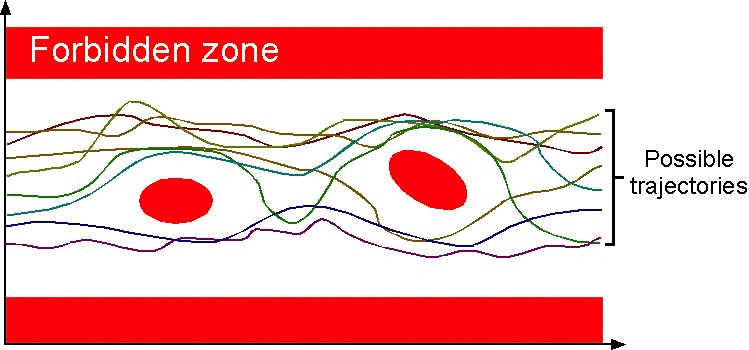
\includegraphics[width=1 \linewidth]{ai-1.png}
        \caption{The \emph{concrete semantics} of programs with \\ \emph{forbidden zones}}
        \label{fig:ai1}
    \end{subfigure}
%
    \hfill
%
    \begin{subfigure}[t]{.49 \linewidth}
        \centering
        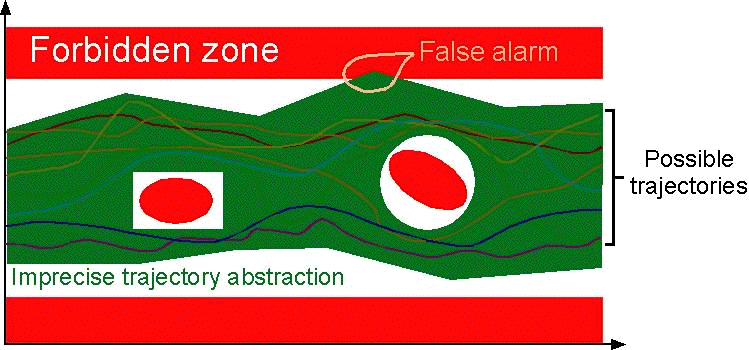
\includegraphics[width=1 \linewidth]{ai-2.png}
        \caption{The \emph{abstract semantics} of programs with \\ \emph{imprecise abstraction}}
        \label{fig:ai2}
    \end{subfigure}

    \caption{An \emph{abstract interpretation} demonstration~\cite{AIInNutshellCousot} (horizontal axes: the time~$ t $; vertical axes: the vector~$ x(t) $~of input, state, and output values of the considered program)}
\end{figure}

\subsection{Components of Abstract Interpretation}
\label{sec:AIComponents}

Before the formal definition of abstract interpretation is given, below are intuitively described basic components of the framework in accordance with~\cite{AICousotWeb, AIBasedFormalMethodsCousot, savAI, programAnalysisNielson}:
\begin{itemize}
    \item \textbf{Abstract Domain}~$ \boldsymbol{Q} $:
        \begin{itemize}
            \item An abstraction of the possible concrete program states (or their parts) in the form of \emph{abstract properties}\footnote{\textbf{Abstract properties} approximate \emph{concrete properties} behaviours.~\cite{AIBasedFormalMethodsCousot}}.

            \item In other words, it is a~set of \emph{abstract states} (or \emph{abstract contexts}), where an abstract state represents a~set of program states reachable at a~particular program location.

            \item For instance, several practical domains have been defined: numerical intervals, polyhedra, octagons, congruences, or various heap domains.
        \end{itemize}

    \item \textbf{Abstract Transformers}~$ \boldsymbol{\tau} $:
        \begin{itemize}
            \item There is a~\emph{transform function}~$ \tau $ for each program operation (instruction) representing the impact of the operation executed on an abstract state.
        \end{itemize}

    \item \textbf{Join Operator}~$ \boldsymbol{\sqcup} $:
        \begin{itemize}
            \item Joins abstract states from individual program branches into a~single one.
        \end{itemize}

    \item \textbf{Widening Operator~$ \boldsymbol{\triangledown} $}:
        \begin{itemize}
            \item Enforces \emph{termination} of the abstract interpretation.

            \item It is used to over-approximate the \emph{least fixed points} of program semantics (it is performed on a~sequence of abstract states at a~certain location).

            \item Usually, the later in the analysis this operator is applied, the more accurate the result is (but the analysis takes more time).
        \end{itemize}

    \item \textbf{Narrowing Operator~$ \boldsymbol{\vartriangle} $}:
        \begin{itemize}
            \item The approximation obtained by the widening operator can be \emph{refined} using the narrowing operator, i.e., it may be used to refine the result of widening.

            \item It is used when a~fixpoint is approximated by the widening operator.
        \end{itemize}
\end{itemize}
Note that neither the widening operator nor narrowing operator are required. However, at least the widening operator is frequently used. The narrowing operator can be sometimes dropped.

\subsection{Formal Definition of Abstract Interpretation}

The definitions below consider notions from \emph{lattice theory}. More information about lattices, functions on lattices, \emph{partial orders}, and set theory can be found, e.g., in~\cite{staticAnalysisMoller, programAnalysisNielson, staticAnalysisRival}.

\begin{definition}[\textbf{Abstract Interpretation}]
    \label{def:AI}
    According to~\cite{AILatticeModelCousot, savAI}, \textbf{abstract interpretation}~$ I $~of a~program~$ P $~with the instruction set $ Instr $~is a~tuple
    $$
        I = (Q, \sqcup, \sqsubseteq, \top, \bot, \tau)
    $$
    where
    \begin{itemize}
        \item $ Q $~is the \emph{abstract domain} (the set of \emph{abstract states}),

        \item $ \sqcup : Q \times Q \rightarrow Q $ is the \emph{join operator} for accumulation of abstract states,

        \item $ \sqsubseteq\ \subseteq Q \times Q $ is an \emph{ordering} defined as $ x \sqsubseteq y \Longleftrightarrow x \sqcup y = y $ where
            \begin{itemize}
                \item $ \langle Q, \sqsubseteq \rangle $ is a~\emph{complete $ \sqcup $-semilattice},
            \end{itemize}

        \item $ \top \in Q $ is the \emph{supremum} of~$ \langle Q, \sqsubseteq \rangle $,

        \item $ \bot \in Q $ is the \emph{infimum} of~$ \langle Q, \sqsubseteq \rangle $\,---\,thus, $ \langle Q, \sqsubseteq \rangle $ is, in fact, a~\emph{complete lattice},

        \item $ \tau : Instr \times Q \rightarrow Q $ defines the \emph{abstract transformers} for specific instructions,
            \begin{itemize}
                \item $ \tau $~must be \emph{monotone}\footnote{Assume two \emph{partially-ordered sets}~$ \langle E, \preceq_E \rangle $ and~$ \langle F, \preceq_F \rangle $, and a~function $ f : E \rightarrow F $. $ f $~is \textbf{monotone} iff $ \forall x, y \in E : x \preceq_E y \Longrightarrow f(x) \preceq_F f(y) $.~\cite{staticAnalysisRival}} on~$ Q $ for each instruction from $ Instr $.
            \end{itemize}
    \end{itemize}
\end{definition}

Using a~so-called \emph{Galois connection}~\cite{AILatticeModelCousot, wideningNarrowingCousot, savAI, staticAnalysisMoller, programAnalysisNielson, staticAnalysisRival}, one can ensure the \emph{soundness} of the abstract interpretation, i.e., the correspondence between the \emph{concrete semantics} and its \emph{abstract semantics} can be formalised by a~Galois connection (also a~so-called pair of \emph{adjoined functions}).
\begin{definition}[\textbf{Galois Connection}]
    If $ \mathcal{P} = \langle P, \preceq \rangle $ and $ \mathcal{Q} = \langle Q, \sqsubseteq \rangle $ are \emph{partially-ordered sets}, then a~quadruple $ \pi = (\mathcal{P}, \alpha, \gamma, \mathcal{Q}) $ is a~\textbf{Galois connection}, written
    $$
        \langle P, \preceq \rangle \overset{\gamma}{\underset{\alpha}\leftrightarrows} \langle Q, \sqsubseteq \rangle
    $$
    iff $ \alpha : P \rightarrow Q $ and $ \gamma : Q \rightarrow P $ are \emph{monotone} functions such that
    $$
        \forall p \in P : \forall q \in Q : \alpha(p) \sqsubseteq q \Longleftrightarrow p \preceq \gamma(q)
    $$
    where~$ P $ is the concrete domain and~$ Q $ is the abstract domain. Furthermore, $ \alpha $~is an \emph{abstraction function}, and~$ \gamma $ is a~\emph{concretisation function}. Consequently, $ \alpha(p) $ is the abstraction of~$ p $, i.e., the most precise approximation of $ p \in P $ in~$ Q $, and $ \gamma(q) $ is the concretisation of~$ q $, i.e., the most imprecise element of~$ P $ which $ q \in Q $ can soundly approximate. A~Galois connection is illustrated in Figure~\ref{fig:galois}.
\end{definition}

\begin{figure}[hbt]
    \centering
    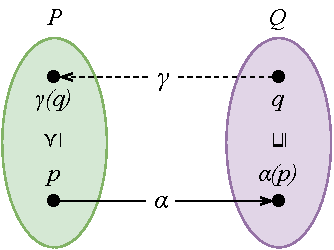
\includegraphics[width=.4 \linewidth]{galois.pdf}
    \caption{An illustration of a~\emph{Galois connection}}
    \label{fig:galois}
\end{figure}

If the abstraction and concretisation functions of the abstract interpretation form a~Galois connection, then applying the abstraction function and concretising the result back yield a~less (or equally) precise result. However, it is a~safe (\emph{conservative}) approximation. That is, formally written, $ \forall p \in P : p \preceq \gamma(\alpha(p)) $. Finally, the abstract interpretation may only over-approximate the concrete semantics (i.e., it is sound) if for each \emph{concrete transformer} (instruction) $ i : P \rightarrow P $ from the instruction set $ Instr $ and the appropriate \emph{abstract transformer} $ \tau : Instr \times Q \rightarrow Q $ respects a~Galois connection. This is $ \forall p \in P : \alpha(i(p)) \sqsubseteq \tau(i, \alpha(p)) $.

\subsection{Fixpoint Approximation~\cite{AILatticeModelCousot, wideningNarrowingCousot, savAI, staticAnalysisMoller, programAnalysisNielson, staticAnalysisRival}}
\label{sec:AIFixpoints}

Most program properties can be represented as \emph{fixpoints}\footnote{Consider a~function~$ f : L \rightarrow L $ on a~set~$ L $. A~\textbf{fixed point} (or \textbf{fixpoint}) of~$ f $ is an element $ l \in L $ iff $ f(l) = l $. The set of all fixpoints of~$ f $ is denoted as $ Fix(f) = \{l \in L\ |\ f(l) = l\} $.~\cite{programAnalysisNielson}}. This reduces the program analysis to the \emph{fixpoint approximation}. The complete analysis of a~program using abstract interpretation can be then viewed as finding the \emph{least/greatest} fixpoint of the equation $ \overline{Q} = \overline{\tau}(\overline{Q}) $, where~$ \overline{Q} $ is a~vector of abstract states and~$ \overline{\tau} $ is an extension of~$ \tau $ to the whole program. This fixpoint equation is then solved iteratively. \emph{Knaster-Tarski theorem}~\cite{tarski} guarantees these fixpoints' existence.

The computation of the most precise abstract fixpoint is not generally guaranteed to \emph{terminate}, in particular, when a~given program contains a~loop (or recursion) and uses an infinite domain (or even finite but very large). In order to enforce or accelerate the convergence, the fixpoint is often over-approximated using the \emph{widening} operator~$ \triangledown $. The approximation may be later refined using the \emph{narrowing} operator~$ \vartriangle $. These two operators are defined below. In practice, the analysis is usually done by iterating the abstract transformers over the \emph{control-flow graph}\footnote{A~\textbf{control-flow graph} (\textbf{CFG}) is a~\emph{directed graph} in which the nodes represent \emph{basic blocks} of the program, and the edges represent control-flow paths among them~\cite{controlFlowAnalysisAllen}. A~basic block is a~\emph{maximal sequence of statements} such that all transfers to it are to the first statement in the sequence, and all statements in the sequence are executed sequentially~\cite{programAnalysisNielson}.} (CFG). The join operator~$ \sqcup $ is applied at program locations where different branches come across. Moreover, the widening operator~$ \triangledown $ is applied at loop junctions (and afterwards, the narrowing operator~$ \vartriangle $ may be used).

\begin{definition}[\textbf{Widening}]
    Assume the abstract interpretation from Definition~\ref{def:AI}. The \textbf{widening operator} over the abstract domain~$ Q $ is a~binary operator~$ \triangledown : Q \times Q \rightarrow Q $ such that $ \forall x, y \in Q : x \sqcup y \sqsubseteq x\,\triangledown\,y $, and for all \emph{increasing chains} $ x_0 \sqsubseteq x_1 \sqsubseteq \ldots\ $, the increasing chain defined by $ y_0 = x_0,\ \ldots\ ,\ y_{i + 1} = y_i\,\triangledown\,x_{i + 1},\ \ldots $ is not \emph{strictly increasing}. Note that the chain eventually stabilises since the result of~$ \triangledown $ is an \emph{upper bound}.
\end{definition}

\begin{definition}[\textbf{Narrowing}]
    Assume the abstract interpretation from Definition~\ref{def:AI}. The \textbf{narrowing operator} over the abstract domain~$ Q $ is a~binary operator~$ \vartriangle : Q \times Q \rightarrow Q $ such that $ \forall x, y \in Q : y \sqsubseteq x \Longrightarrow y \sqsubseteq x \vartriangle y \sqsubseteq x $, and for all \emph{decreasing chains} $ x_0 \sqsupseteq x_1 \sqsupseteq \ldots\ $, the decreasing chain defined by $ y_0 = x_0,\ \ldots\ ,\ y_{i + 1} = y_i \vartriangle x_{i + 1},\ \ldots $ is not \emph{strictly decreasing}. Note that the chain eventually stabilises since the result of~$ \vartriangle $ is a~\emph{lower bound}.
\end{definition}


\section{\texorpdfstring{Facebook Infer\,---\,Static Analysis Framework}{Facebook Infer - Static Analysis Framework}}
\label{sec:fbinfer}

This section describes the principles and features of \emph{Facebook Infer}. The description is based on information provided at the Facebook Infer's website\footnote{The \textbf{Facebook Infer's} website: \url{https://fbinfer.com}.} and in~\cite{inferAISpeech}.

\begin{figure}[hbt]
    \centering
    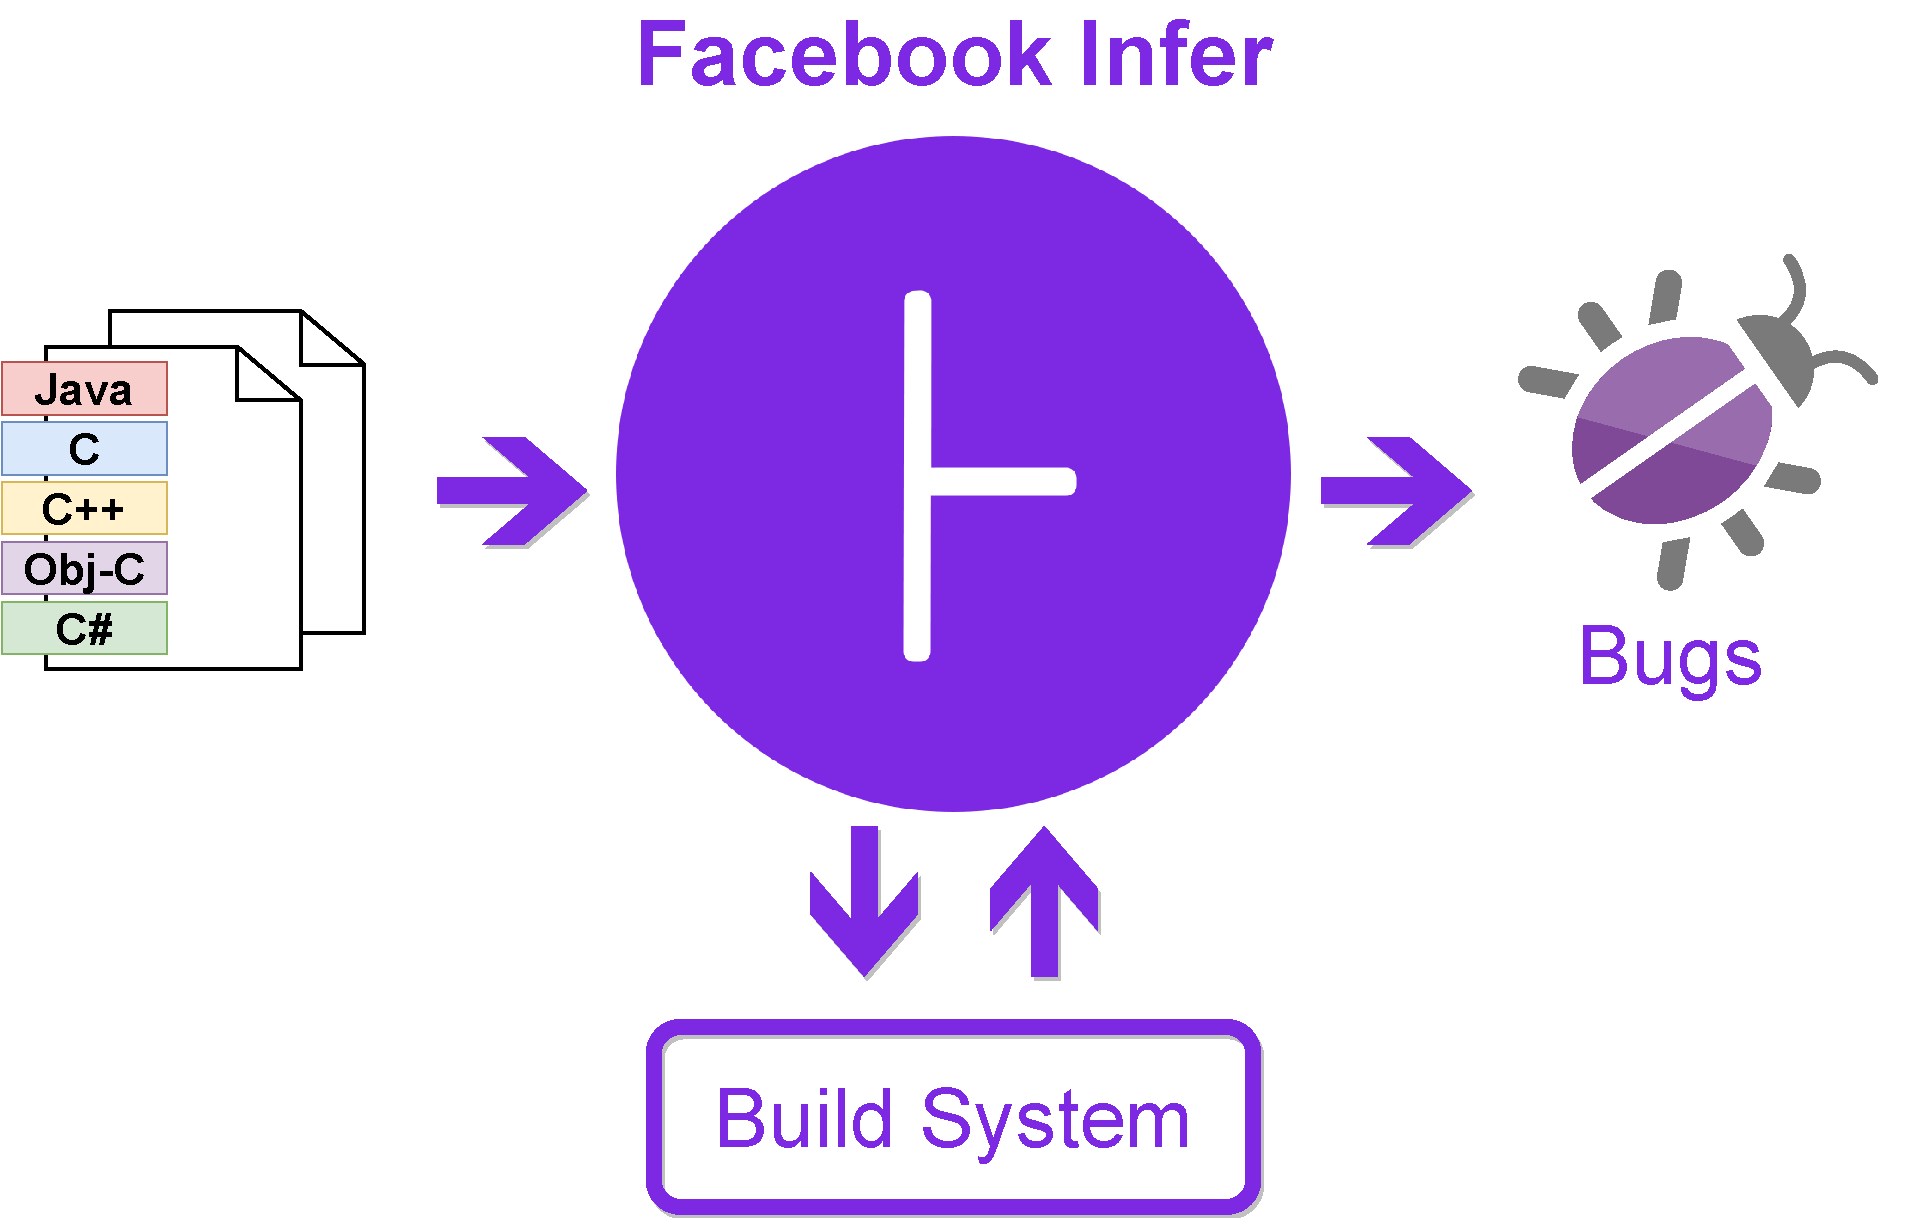
\includegraphics[width=.5 \linewidth]{infer.pdf}
    \caption{Static analysis in \emph{Facebook Infer}}
    \label{fig:infer}
\end{figure}

Facebook Infer is an \emph{open-source}\footnote{The \textbf{Facebook Infer's open-source repository} at GitHub: \url{https://github.com/facebook/infer}.} \emph{static analysis framework}, which can discover various kinds of software bugs and which stress the \emph{scalability} of the analysis. The Facebook Infer's basic usage is illustrated in Figure~\ref{fig:infer}. A~more detailed explanation of its architecture is given in Section~\ref{sec:fbinferArch}. Facebook Infer is implemented in \emph{OCaml}\footnote{The \textbf{OCaml's} website: \url{https://ocaml.org}.}\,---\,a~\emph{functional} programming language, also supporting \emph{imperative} and \emph{object-oriented} paradigms. Further details about OCaml can be found in the book~\cite{realWorldOCaml}. Infer has initially been a~rather specialised tool focused on \emph{sound verification} of the absence of \emph{memory safety violations}, which was first published in the well-known paper~\cite{inferBiabduction}. Once Facebook has purchased it, its scope significantly widened and abandoned the focus on sound analysis only.

Facebook Infer can analyse programs written in the following languages: C, C++, Java, Objective-C (and support for~C\# has been recently implemented~\cite{inferCSharp}). Moreover, it is possible to extend Facebook Infer's \emph{frontend} for supporting other languages. Currently, Facebook Infer contains many analyses focusing on various kinds of bugs, e.g., \emph{Inferbo}~\cite{inferboOnline} (buffer overruns); \emph{RacerD}~\cite{racerD, racerDOnline, staticRaceDetectorTruePositives} (data races); and other analyses that check for buffer overflows, some forms of deadlocks and starvation, null-dereferencing, memory leaks, resource leaks, etc. Since Facebook Infer is a~relatively popular and open-source framework, many experimental analysers arise pretty often. For instance, the promising experimental deadlock checker L2D2~\cite{marcinBP} has been implemented at FIT BUT not long ago.

\subsection{Abstract Interpretation in Facebook Infer}
\label{sec:fbinferAI}

Facebook Infer is a~general framework for static analysis of programs, and it is based on \emph{abstract interpretation}. Despite the original approach taken from~\cite{inferBiabduction}, Facebook Infer aims to find bugs rather than perform \emph{formal verification}. It is still possible to propose \emph{sound} and \emph{complete} analyses in the framework. However, the majority of the checkers already implemented in Facebook Infer are both unsound and incomplete.

It can be used to develop new sorts of \emph{compositional} and \emph{incremental} analysers quickly (both \emph{intraprocedural} and \emph{interprocedural}~\cite{programAnalysisNielson}) based on the concept of function \emph{summaries}. In general, a~summary~$ \chi $ represents a~set of \emph{pre-condition}/\emph{post-condition} pairs for a~function. In particular, it records under which pre-condition a~function can be performed leading to a~given post-condition. Formally, it can be described using \emph{Hoare triples}~\cite{hoare}, because it can be viewed as a~triple $ \{P\}\ S\ \{R\} $, where~$ P $ is a~pre-condition, $ S $ is a~program (or a~single statement/command)\footnote{In Facebook Infer's summaries considered as Hoare triples, $ S $ is usually one function.}, and~$ R $ is a~description of the result of the execution of~$ S $ (i.e., a~post-condition). In theory, $ P $ and $ R $ are considered formulae in a~suitable logic. The triple may be interpreted as follows. Suppose~$ S $ is executed from a~state satisfying~$ P $, and the execution of~$ S $ terminates. In that case, the program state after~$ S $ terminates satisfies~$ R $. However, in practice, a~summary is a~custom data structure that may be used for storing any information resulting from the analysis of particular functions. Usually, a~summary consists of the relevant parts of \emph{abstract states} for a~particular analysis.

Facebook Infer generally does not compute the summaries during the analysis along the CFG as it is done in classical analyses based on the concepts from~\cite{DFAGraphReach, DFAApproaches}. Instead, Facebook Infer performs the analysis of a~program \emph{function-by-function along the call-tree}, starting from its leaves (demonstrated later in Example~\ref{ex:AIAnalysis}). Therefore, a~function is analysed, and a~summary is computed without knowledge of the call context. Then, the summary of the function is used at all its call sites. It is needed to deduce under which pre-conditions a~function can produce post-conditions appropriate for the given analysis. Since the summaries do not differ for different contexts, each function is analysed precisely once, and the analysis becomes more scalable, but it can lead to a~loss of accuracy. However, of course, it is more troublesome to propose such a~\emph{bottom-up} analysis.

In order to create a~new intraprocedural analyser in Facebook Infer, it is required to define the following (the listed items are described in more detail in Section~\ref{sec:AI}):
\begin{enumerate}
    \item The \emph{abstract domain}~$ Q $, i.e., the type of \emph{abstract states}.

    \item The \emph{ordering operator}~$ \sqsubseteq $, i.e., an ordering of abstract states.

    \item The \emph{join} operator~$ \sqcup $, i.e., the way of joining two abstract states.

    \item The \emph{widening} operator~$ \triangledown $, i.e., the way how to enforce termination of the computation.

    \item The \emph{transfer functions}~$ \tau $, i.e., transformers that take an abstract state as an input and produce an abstract state as an output.
\end{enumerate}
Furthermore, to create an interprocedural analyser, it is required to define additionally:
\begin{enumerate}
    \item The type of function summaries~$ \chi $.

    \item The logic for using summaries in transfer functions and the logic for transforming an intraprocedural abstract state to a~summary.
\end{enumerate}

An important Facebook Infer's feature, which improves its scalability, is the \emph{incrementality} of the analysis. It allows one to analyse separate code changes only, instead of analysing the whole codebase. It is more suitable for extensive and variable projects where ordinary analysis is not feasible. The incrementality is based on \emph{re-using summaries} of functions for which there is no change in them neither in the functions transitively invoked from them, as shown in Example~\ref{ex:AIAnalysis} later on.

\subsection{Architecture of the Infer.AI Framework}
\label{sec:fbinferArch}

The architecture of the abstract interpretation framework of Facebook Infer (\textbf{Infer.AI}) may be split into three major parts, as demonstrated in Figure~\ref{fig:inferArch}: the \emph{frontend}, an \emph{analysis scheduler} (and the \emph{results database}), and a~set of \emph{analyser plugins}.

The frontend compiles input programs into the \emph{Smallfoot Intermediate Language} (SIL) and represents them as a~CFG. There is a~separate CFG representation for each analysed function. Nodes of this CFG are formed as SIL instructions. The SIL language consists of the following underlying instructions:
\begin{itemize}
    \item \texttt{LOAD}\,---\,reading into a~temporary variable;

    \item \texttt{STORE}\,---\,writing to a~program variable, field of a~structure, or array;

    \item \texttt{CALL}\,---\,a~function call;

    \item \texttt{PRUNE~e}\,---\,the evaluation of an expression~\texttt{e} in a~condition, cycle, etc.
\end{itemize}
The frontend allows one to propose \emph{language-independent} analyses (to a~certain extent) because it supports input programs to be written in multiple languages.

\begin{figure}[hbt]
    \centering
    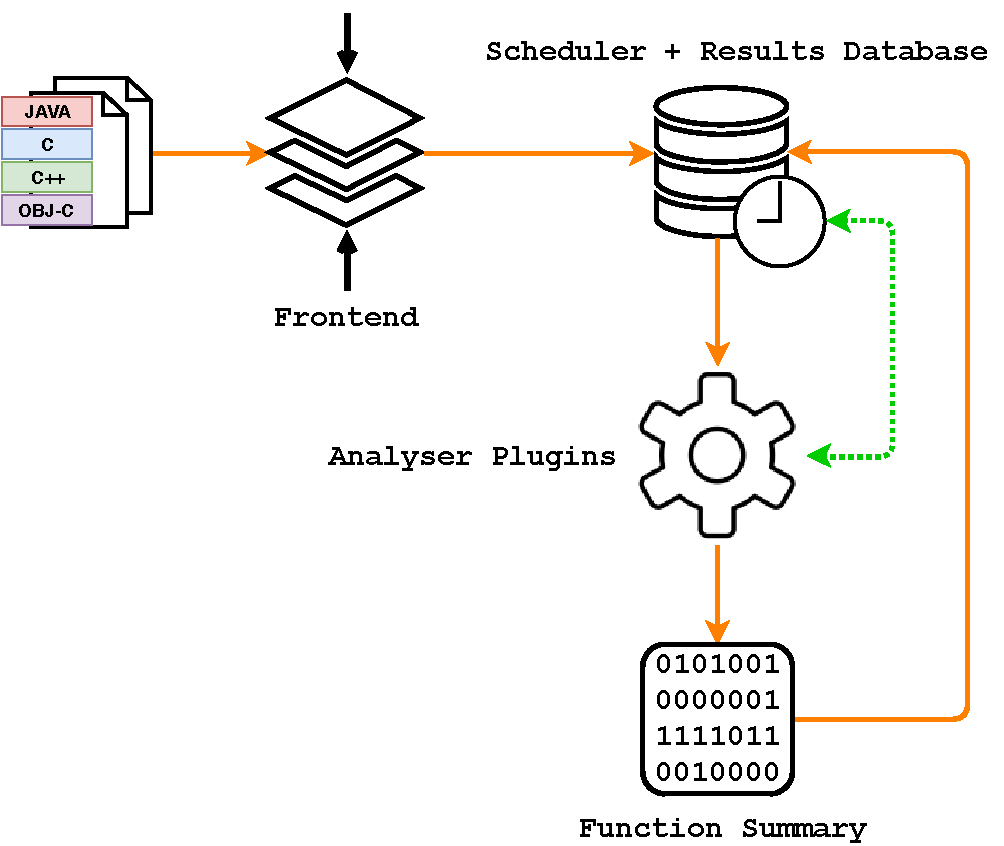
\includegraphics[width=.65 \linewidth]{infer-architecture.pdf}
    \caption{The \emph{architecture} of the Facebook Infer's \emph{abstract interpretation framework}~\cite{harmimBP}}
    \label{fig:inferArch}
\end{figure}

\begin{wrapfigure}{r}{.45 \linewidth}
    \centering
    \vspace{-1em}
    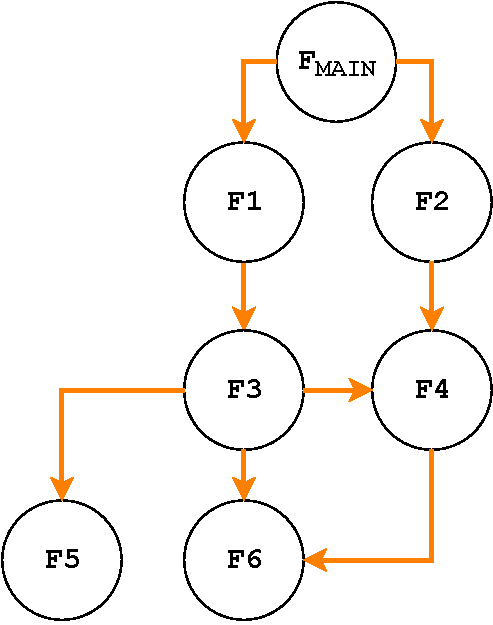
\includegraphics[width=.25 \textwidth]{infer-call-graph.pdf}
    \caption{A~\emph{call graph} for an illustration of Facebook Infer's \emph{analysis process}~\cite{harmimBP}}
    \vspace{-2em}
    \label{fig:inferCallGraph}
\end{wrapfigure}
The next part of the architecture is the scheduler, which defines the order of the analysis of single functions according to the appropriate \emph{call graph}\footnote{A~\textbf{call graph} is a~\emph{directed graph} describing call dependencies among functions.}. The scheduler also checks if it is possible to simultaneously analyse some functions, allowing Facebook Infer to run the analysis in parallel.

\begin{example}
    \label{ex:AIAnalysis}
    For demonstrating the order of the analysis in Facebook Infer and its incrementality, assume the call graph given in Figure~\ref{fig:inferCallGraph}. At first, leaf functions \texttt{F5} and \texttt{F6} are analysed. Further, the analysis goes on towards the root of the call graph\,---\,\texttt{F\textsubscript{MAIN}}, while considering the dependencies denoted by the edges. This order ensures that a~summary is available once a~nested function call is abstractly interpreted within the analysis. When there is a~subsequent code change, only directly changed functions and all the functions up the call path are re-analysed. For instance, if there is a~change of source code of function \texttt{F4}, Facebook Infer triggers re-analysis of functions \texttt{F4}, \texttt{F2}, and \texttt{F\textsubscript{MAIN}} only.
\end{example}

The last part of the architecture consists of analyser plugins. Each plugin performs some analysis by interpreting SIL instructions. The result of the analysis of each function (function summary) is stored in the results database. The interpretation of SIL instructions (\emph{commands}) is made using the \emph{abstract interpreter} (also called the \emph{control interpreter}) and \emph{transfer functions} (also called the \emph{command interpreter}). The transfer functions take a~previously generated abstract state of an analysed function as an input, and by applying the interpreting command, produce a~new abstract state. The abstract interpreter interprets the command in an abstract domain according to the CFG. This workflow is shown in a~simplified form in Figure~\ref{fig:inferAnalysis}.

\begin{figure}[hbt]
    \centering
    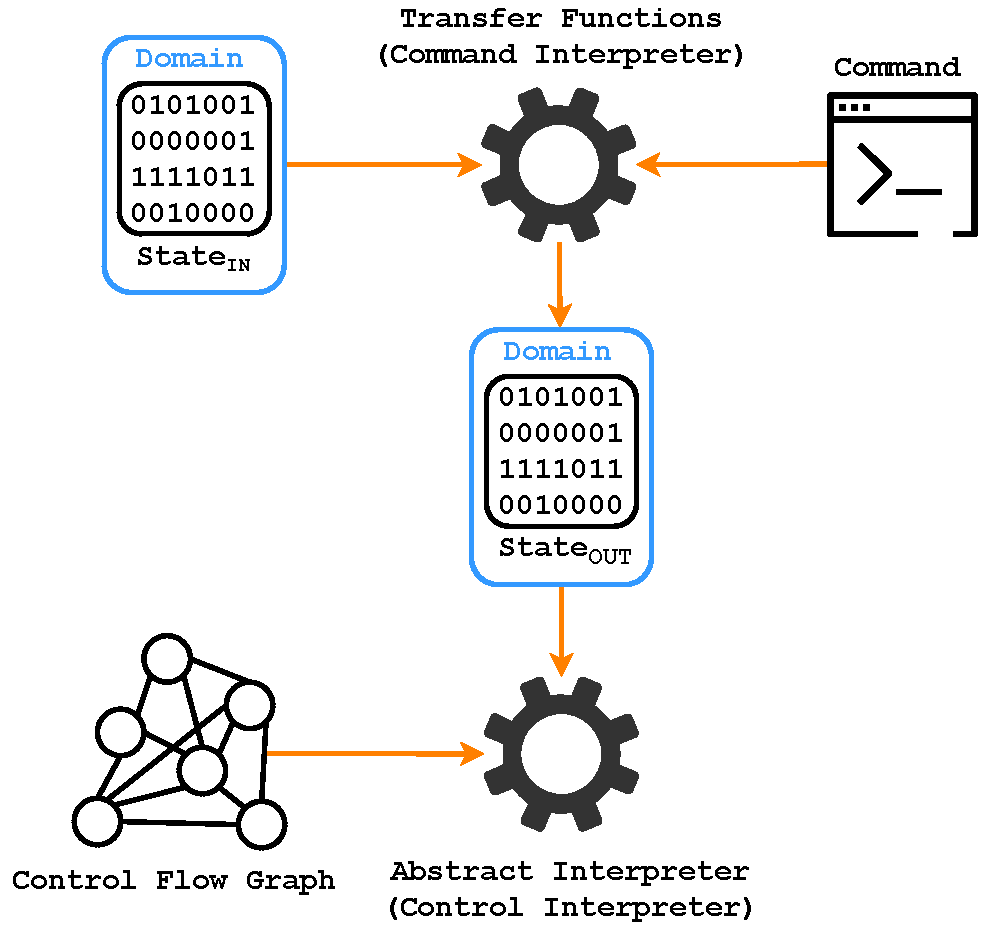
\includegraphics[width=.65 \linewidth]{infer-analysis.pdf}
    \caption{The Facebook Infer's \emph{abstract interpretation process}~\cite{harmimBP}}
    \label{fig:inferAnalysis}
\end{figure}


\section{Contracts for Concurrency}
\label{sec:contracts}

This section introduces the concept of \emph{contracts for concurrency}~\cite{contracts2017, contracts2015}. Examples and listings in the section are pieces of programs written in the C~language.

Respecting the \emph{protocol} of a~software module\,---\,that defines which \emph{sequences of functions} are legal to invoke\,---\,is one of the requirements for the correct behaviour of the module. For example, a~module that deals with a~file system typically requires that a~programmer using this module should call a~function \texttt{open} at first, followed by an optional number of functions \texttt{read} and \texttt{write}, and at last, call a~function \texttt{close}. A~program utilising such a~module that does not follow this protocol is erroneous. The methodology of \emph{design by contract}~\cite{contract} requires programs to meet such well-defined behaviours.~\cite{contracts2015}

In \emph{concurrent programs}, contracts for concurrency allow one\,---\,in the simplest case\,---\,to specify sequences of functions that are needed to be \emph{executed atomically} in order to avoid \emph{atomicity violations}. In general, contracts for concurrency specify sets of sequences of calls called \emph{spoilers} and sets of sequences of calls called \emph{targets}. It is then required that no target overlaps fully with any spoiler. A~developer may manually specify such contracts or automatically generate them by a~program (analyser). These contracts can be used to verify the correctness of programs as well as they can serve as helpful documentation.

Section~\ref{sec:contractsBasic} defines the notion of \emph{basic contracts for concurrency}. Further, Section~\ref{sec:contractsParams} defines contracts extended to consider the \emph{data flow} between functions, where a~sequence of function calls must be atomic only if they handle the same data. Finally, Section~\ref{sec:contractsSpoilers} presents those mentioned above more general contracts for concurrency with spoilers and targets, which essentially extend the basic contracts with some \emph{contextual information}.

\subsection{Basic Contracts for Concurrency}
\label{sec:contractsBasic}

In~\cite{contracts2017, contracts2015}, a~\emph{basic contract for concurrency} is formally defined as follows. Let~$ \Sigma_\mathbb{M} $ be a~set of all function names of a~software module~$ \mathbb{M} $. A~contract is a~set~$ \mathbb{R} $ of \emph{clauses}, where each clause $ \varrho \in \mathbb{R} $ is a~\emph{star-free regular expression}\footnote{\textbf{Star-free regular expressions} are regular expressions that use only the \emph{concatenation operator} and the \emph{alternative operator} (\texttt{|}), without the \emph{Kleene star operator} (\texttt{\textsuperscript{*}}).} over~$ \Sigma_\mathbb{M} $. A~\emph{contract violation} occurs if any of the sequences expressed by the contract clauses are interleaved with the execution of functions from~$ \Sigma_\mathbb{M} $. In other words, each sequence specified by any clause~$ \varrho $ must be executed atomically. Otherwise, there is a~violation of the contract. The number of sequences defined by a~contract is finite since the contract is a~union of \emph{star-free languages}.

\begin{example}
    \label{ex:contractsBasic}
    Consider the following example from~\cite{contracts2017, contracts2015}. Assume a~module~$ \mathbb{M} $ implementing a~resizable array of integers with the following interface functions $ \Sigma_\mathbb{M} = \{ $\texttt{add, contains, index\_of, get, set, remove, size}$ \} $ defined as:
    \begin{enumerate}[label=]
        \tt

        \item \kw{void} add(\kw{int} *array, \kw{int} element)

        \item \kw{bool} contains(\kw{int} *array, \kw{int} element)

        \item \kw{int} index\_of(\kw{int} *array, \kw{int} element)

        \item \kw{int} get(\kw{int} *array, \kw{int} index)

        \item \kw{void} set(\kw{int} *array, \kw{int} index, \kw{int} element)

        \item \kw{void} remove(\kw{int} *array, \kw{int} index)

        \item \kw{int} size(\kw{int} *array)
    \end{enumerate}
    The module's contract contains clauses $ \mathbb{R} = \{\varrho_1, \varrho_2, \varrho_3, \varrho_4\} $ such that:
    \begin{enumerate}[label={($ \varrho_{\arabic*} $)}]
        \item \texttt{contains index\_of}
            \begin{addmargin}[1em]{0em}
                The execution of \texttt{contains} followed by the execution of \texttt{index\_of} should be atomic. Otherwise, the program may fail to get the index because after checking the presence of an element in an array, it can be removed by some concurrent thread.
            \end{addmargin}

        \item \texttt{index\_of (\,get\,|\,set\,|\,remove\,)}
            \begin{addmargin}[1em]{0em}
                The execution of \texttt{index\_of} followed by the execution of \texttt{get}, \texttt{set}, or \texttt{remove} should be atomic. Otherwise, the received index may be outdated when applied to address an array element because a~concurrent modification of the array may shift the element's position.
            \end{addmargin}

        \item \texttt{size (\,get\,|\,set\,|\,remove\,)}
            \begin{addmargin}[1em]{0em}
                The execution of \texttt{size} followed by the execution of \texttt{get}, \texttt{set}, or \texttt{remove} should be atomic. Otherwise, an array may be empty when accessing it because of a~concurrent change of the array. This can be an issue since a~given index is not in a~valid range anymore (e.g., testing \texttt{index < size}).
            \end{addmargin}

        \item \texttt{add index\_of}
            \begin{addmargin}[1em]{0em}
                The execution of \texttt{add} followed by the execution of \texttt{index\_of} should be atomic. Otherwise, the added element needs no longer exist in an array.
            \end{addmargin}
    \end{enumerate}
\end{example}

\subsection{Contracts for Concurrency with Parameters}
\label{sec:contractsParams}

The above definition of basic contracts for concurrency is quite limited in some circumstances and can consider valid programs as erroneous (i.e., \emph{false alarms} may be reported). Hence, in this section, there is introduced an extension of basic contracts\,---\,\emph{contracts for concurrency with parameters} (defined in~\cite{contracts2017, contracts2015})\,---\,which takes into consideration the \emph{data flow} within function calls.

\begin{example}
    Consider the following example from~\cite{contracts2017, contracts2015}, given Listing~\ref{list:contractsReplace}. There is the function \texttt{replace} that replaces item~\texttt{a}~in an array by item~\texttt{b}. The implementation of this function comprises two atomicity violations:
    \begin{enumerate}
        \item when \texttt{index\_of} is invoked, item~\texttt{a} does not need to be in the array anymore; and

        \item the acquired index can be obsolete when \texttt{set} is executed.
    \end{enumerate}
    A~basic contract could cover this scenario by the following clause:
    $$
        (\varrho_5)\ \text{\texttt{contains index\_of set}}
    $$
    It can be obtained from the composition of clauses~$ \varrho_1 $ and~$ \varrho_2 $. Nevertheless, this definition is too restrictive because the functions are required to be executed atomically only if \texttt{contains} and \texttt{index\_of} have the same arguments \texttt{array} and \texttt{element}; \texttt{index\_of} and \texttt{set} have the same argument \texttt{array}; and the returned value of \texttt{index\_of} is used as the argument \texttt{index} of the function \texttt{set}.
\end{example}

\begin{lstlisting}[style=c, label={list:contractsReplace}, float=hbt, caption={An example of an atomicity violation with \emph{data dependencies}~\cite{contracts2017, contracts2015}}]
void replace(int *array, int a, int b)
{
    if (contains(array, a))
    {
        int index = index_of(array, a);
        set(array, index, b);
    }
}
\end{lstlisting}

To respect function call \emph{parameters} and \emph{return values} of functions in contracts, the basic contracts are extended by dependencies among functions in~\cite{contracts2017, contracts2015} as follows. Function call parameters and return values are expressed as \emph{meta-variables}. Further, if a~contract should be required to be observed exclusively if the same object emerges as an argument or as the return value of multiple calls in a~given call sequence, it may be denoted by using the same meta-variable at the position of all these occurrences of parameters and return values.

Clause~$ \varrho_5 $~can be extended as follows (repeated application of meta-variables \texttt{X/Y/Z} requires the same objects $ o_1/o_2/o_3 $ to be used at the positions of \texttt{X/Y/Z}, respectively; and the underscore indicates a~\emph{free meta-variable} that does not restrict
the contract clause):
$$
    (\varrho^\prime_5)\ \text{\texttt{contains(X,\,Y) Z\,=\,index\_of(X,\,Y) set(X,\,Z,\,\_)}}
$$

\begin{example}
    With the extension described above, it is possible to extend the contract from Example~\ref{ex:contractsBasic} to capture the dependencies between function calls as follows:
    \begin{enumerate}[label={($ \varrho^\prime_{\arabic*} $)}]
        \tt

        \item contains(X,\,Y) index\_of(X,\,Y)

        \item Y\,=\,index\_of(X,\,\_) (\,get(X,\,Y)\,|\,set(X,\,Y,\,\_)\,|\,remove(X,\,Y)\,)

        \item size(X) (\,get(X,\,\_)\,|\,set(X,\,\_,\,\_)\,|\,remove(X,\,\_)\,)

        \item add(X,\,Y) index\_of(X,\,Y)
    \end{enumerate}
\end{example}

\subsection{Contracts for Concurrency with Spoilers}
\label{sec:contractsSpoilers}

Interleaving a~sequence of function calls from a~contract clause (considering the basic contracts for concurrency or contracts with parameters) with some function calls of a~given module can cause atomicity violations. At the same time, this is not the case for some other function calls from the module. However, this is not possible to describe in the contracts introduced so far. For instance, clause ($ \varrho_1 $) \texttt{contains index\_of} requires that this sequence of calls must always be performed atomically, i.e., it does not matter which functions are executed by other threads. Thus, interleaving the execution of this sequence with, e.g., \texttt{remove} or \texttt{get} is a~contract violation. However, in effect, only the execution of \texttt{remove} may be problematic, while the execution of \texttt{get} may not.

The paper~\cite{contracts2017} proposes a~solution to the above issue\,---\,an extension of the basic contracts for concurrency with \emph{contextual information}\,---\,allowing one to describe in which context the contract clauses should be enforced. Each clause of the basic contract is now called \emph{target}. For each target, there is a~set of so-called \emph{spoilers} that restrict its application. That is, a~spoiler is a~sequence of function calls that can violate its target. In the end, it has to be ensured that each target is executed atomically w.r.t. its spoilers. Assuming the earlier example, let \texttt{contains index\_of} be the target clause. Then, a~possible spoiler is \texttt{remove}. The syntax for this description is as follows: \texttt{contains index\_of}\ $ \leftsquigarrow $\ \texttt{remove}.

Formally, let~$ \Sigma_\mathbb{M} $ be a~set of all function names of a~software module~$ \mathbb{M} $. Further, let~$ \mathbb{R} $ be a~set of \emph{target clauses}, where each clause $ \varrho \in \mathbb{R} $ is a~star-free regular expression over~$ \Sigma_\mathbb{M} $. Let~$ \mathbb{S} $ be a~set of \emph{spoiler clauses}, where each clause $ \sigma \in \mathbb{S} $ is a~star-free regular expression over~$ \Sigma_\mathbb{M} $. Moreover, let $ \Sigma_\mathbb{R} \subseteq \Sigma_\mathbb{M} $ and $ \Sigma_\mathbb{S} \subseteq \Sigma_\mathbb{M} $ be the alphabets of function names used in the target or spoiler clauses, respectively. Then, a~contract is a~relation $ \mathbb{C} \subseteq \mathbb{R} \times \mathbb{S} $, which states for each target the spoilers that can cause atomicity violations. One spoiler may violate more than one target, and, on the contrary, one target may be violated by more than one spoiler. A~contract is violated iff any executed sequence expressed by a~target $ \varrho \in \mathbb{R} $ is \emph{completely interleaved} with the execution of the sequence representing its spoiler, i.e., $ \sigma \in \mathbb{C}(\varrho) $. A~target sequence~$ r $ is completely interleaved by a~spoiler sequence~$ s $ iff the execution of~$ r $ \emph{starts before} the execution of~$ s $, and the execution of~$ s $ \emph{ends before} the execution of~$ r $. \emph{Partial interleavings} of targets and spoilers are here not taken into account to cause an error. However, if needed, this can be resolved by adding a~new target clause with an appropriate spoiler. Whether a~sequence is executed before another one is, is defined using the so-called \emph{\uv{happened before} relation}~($ \xrightarrow{\mathtt{hb}} $)~\cite{lamportHb}. Complete interleaving is illustrated in Figure~\ref{fig:contract1}, and partial interleavings are shown in Figures~\ref{fig:contract2} and~\ref{fig:contract3}.

\begin{figure}[hbt]
    \centering

    \begin{subfigure}[t]{.31 \linewidth}
        \centering
        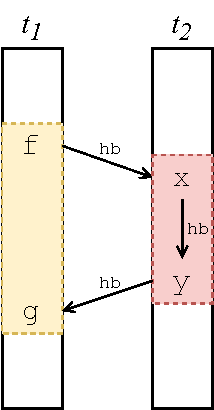
\includegraphics[width=.55 \linewidth]{contract1.pdf}
        \caption{\emph{Complete interleaving}: \\ the contract is violated}
        \label{fig:contract1}
    \end{subfigure}
%
    \hfill
%
    \begin{subfigure}[t]{.31 \linewidth}
        \centering
        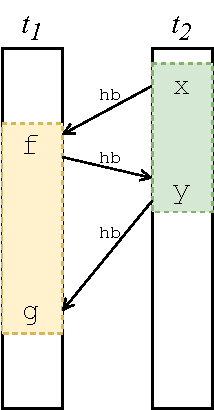
\includegraphics[width=.55 \linewidth]{contract2.pdf}
        \caption{\emph{Partial interleaving}: \\ the contract is not violated \\ ($ s $ \emph{started before}~$ r $)}
        \label{fig:contract2}
    \end{subfigure}
%
    \hfill
%
    \begin{subfigure}[t]{.31 \linewidth}
        \centering
        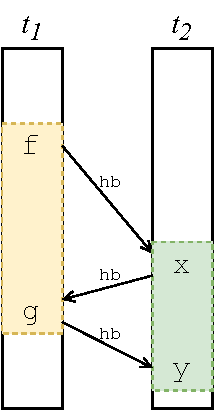
\includegraphics[width=.55 \linewidth]{contract3.pdf}
        \caption{\emph{Partial interleaving}: \\ the contract is not violated \\ ($ s $ \emph{ended after}~$ r $)}
        \label{fig:contract3}
    \end{subfigure}

    \caption{A~\emph{contract violation} demonstration with \emph{target and spoiler interleavings}. In each sub-figure, a~thread~$ t_1 $ executes a~target sequence $ r = \mathtt{f\ g} $ and a~thread~$ t_2 $ executes a~spoiler sequence $ s = \mathtt{x\ y} $. Consequently, there is the following contract: $ \mathtt{f\ g}\ \leftsquigarrow\ \mathtt{x\ y} $~\cite{muzikovskaBP}}
\end{figure}

\begin{example}
    With the extension of spoilers, the contract from Example~\ref{ex:contractsBasic} can be refined with contextual information to refuse \emph{unsafe interleavings} as follows (all other interleavings, not described by spoilers, are deemed  safe):
    \begin{enumerate}[label={($ \varrho^{\prime\prime}_{\arabic*} $)}]
        \tt

        \item contains index\_of\ $ \leftsquigarrow $\ remove\,|\,set

        \item index\_of (\,get\,|\,set\,|\,remove\,) $ \leftsquigarrow $\ remove\,|\,set

        \item size (\,get\,|\,set\,|\,remove\,) $ \leftsquigarrow $\ remove

        \item add index\_of $ \leftsquigarrow $\ remove\,|\,set
    \end{enumerate}
\end{example}

Lastly, it is possible to combine the extension of contracts for concurrency with spoilers and with parameters. The following clause can demonstrate it:
$$
    \text{\texttt{Y\,=\,index\_of(X,\,\_) get(X,\,Y)}}\ \leftsquigarrow\ \text{\texttt{remove(X,\,\_)}}
$$
The clause requires sequences of \texttt{index\_of} and \texttt{get} to be performed atomically, but only when working with the same element~\texttt{X} and index~\texttt{Y}, and only w.r.t. the concurrent execution of \texttt{remove}. Note that the argument \texttt{index} of \texttt{remove} is not restricted because any concurrent removal may produce an atomicity violation\,---\,by either removing an element on index~\texttt{Y} or by shifting its position.



%===============================================================================



\chapter{\texorpdfstring{Atomer\,---\,Atomicity Violations Detector}{Atomer - Atomicity Violations Detector}}
\label{chap:atomer}

This chapter describes the principles and limitations of the basic version of the \emph{Atomer static analyser} proposed as a~module of \emph{Facebook Infer} (introduced in Section~\ref{sec:fbinfer}) for finding some forms of \emph{atomicity violations}. Atomer was proposed and in detail described in the bachelor's thesis~\cite{harmimBP} of the author of this thesis. Therefore, naturally, the description in Section~\ref{sec:atomerDesing} is based on the mentioned thesis. Already existing solutions in this area (besides Atomer) are discussed in Section~\ref{sec:atomerRelatedWork}. In particular, it deals with other existing approaches and tools for finding atomicity violations, their advantages, disadvantages, features, availability, and so on. In Section~\ref{sec:atomerLimits}, there are discussed limitations and shortcomings of Atomer. Some of the thoughts mentioned in this section are taken into consideration already in~\cite{harmimBP}.


\section{Related Work}
\label{sec:atomerRelatedWork}

Atomer is slightly inspired by ideas from~\cite{contracts2017, contracts2015}. In these papers, there is described a~proposal and implementation of a~\emph{static} approach for finding \emph{atomicity violations of sequences of function calls}, which is based on \emph{grammars} and \emph{parsing trees}. Note that in the paper~\cite{contracts2017}, there is also described and implemented a~\emph{dynamic} approach for the validation. The authors of these papers implemented a~stand-alone prototype static analyser called \emph{Gluon}\footnote{\textbf{Gluon} is a~tool that implements a~\emph{static} approach for finding \emph{atomicity violations of sequences of function calls} in Java programs. It is available at \url{https://github.com/trxsys/gluon}.} for analysing programs written in Java. To the best author's knowledge, Gluon is the only static analyser that tries to go in a~similar direction as Atomer does. Gluon led to some promising experimental results, but the \emph{scalability} of Gluon was still limited.\footnote{Some of the experiments performed by Gluon are also similarly performed by Atomer, which is discussed in Sections~\ref{sec:expGluon}, \ref{sec:expReal}.} Moreover, Gluon is no more actively developed, and it is not easy to use. Despite all author's efforts, it was not put into operation. Above that, the authors themselves note that the code of Gluon is very ad hoc, and many things are hard-coded in it. These facts, in fact, inspired the decision that eventually led to the implementation of the first version of Atomer, namely, to get inspired by the ideas of~\cite{contracts2017, contracts2015} but reimplement them in \emph{Facebook Infer}, redesigning it in accordance with the principles of Facebook Infer, which should make the resulting tool more scalable. In the end, however, due to adapting the analysis to the context of Facebook Infer, the implementation of Atomer's analysis is significantly different from~\cite{contracts2017, contracts2015}, as is presented in Chapter~4 of~\cite{harmimBP}. Furthermore, unlike Gluon, a~new version of Atomer is capable of analysing a~much wider range of programs because it also supports other languages than Java, and it supports more advanced \emph{locking mechanisms}. On the other hand, Gluon implements \emph{extended contracts for concurrency} (see Sections~\ref{sec:contractsParams}, \ref{sec:contractsSpoilers}) that consider \emph{data flow} within functions and \emph{contextual information}, while Atomer implements only the idea of \emph{basic contracts for concurrency} (see Section~\ref{sec:contractsBasic}). These extended contracts should improve the precision of the analysis. Nonetheless, it is the author's future work to implement the extended contracts in Atomer as well.

In Facebook Infer, there is already implemented analysis called \emph{Lock Consistency Violation}\footnote{\textbf{Lock Consistency Violation} is an \emph{atomicity violations} analysis implemented in \emph{Facebook Infer}. It is described at \url{https://fbinfer.com/docs/all-issue-types\#lock_consistency_violation}.}. It is a~part of \emph{RacerD}~\cite{racerD, racerDOnline, staticRaceDetectorTruePositives}. This analysis finds atomicity violations in C++ and Objective-C programs for \emph{reads/writes} on single variables required to be executed atomically. Atomer is different; it finds atomicity violations for \emph{sequences of functions} required to be executed atomically. Moreover, Atomer tries to automatically determine which sequences should indeed be executed atomically.


\section{Design of Atomer and Its Principles}
\label{sec:atomerDesing}

Atomer concentrates on checking the \emph{atomicity of the execution of certain sequences of function calls}, which is often required for \emph{concurrent programs'} correct behaviour. In principle, Atomer is based on the assumption that sequences of function calls executed \emph{atomically once} should probably be executed \emph{always atomically}.

The proposal of Atomer is based on the concept of \emph{contracts for concurrency} described in Section~\ref{sec:contracts}. In particular, the proposal considers the \emph{basic contracts} described in Section~\ref{sec:contractsBasic}. Neither the contracts extended by \emph{parameters} explained in Section~\ref{sec:contractsParams} nor the contracts extended by \emph{spoilers} and \emph{targets} described in Section~\ref{sec:contractsSpoilers} are so far taken into account.

In general, basic contracts for concurrency allow one to define sequences of functions required to be executed atomically, as explained in more detail in Section~\ref{sec:contracts}. Atomer is able to automatically derive candidates for such contracts and then verify whether the contracts are fulfilled. In other words, Atomer can both automatically derive those sequences that are sometimes executed atomically as well as subsequently check whether they are indeed always executed atomically. Both of these steps are done statically. The proposed analysis is thus divided into two parts (\emph{phases of the analysis} that are in-depth described in the sections below and illustrated in Figure~\ref{fig:atomerPhasesSequences}):
\begin{enumerate}[label={\textbf{Phase~\arabic*}:}, leftmargin=6.5em]
    \item Detection of (likely) \emph{atomic sequences}.

    \item Detection of \emph{atomicity violations} (violations of the atomic sequences).
\end{enumerate}

\begin{figure}[hbt]
    \centering
    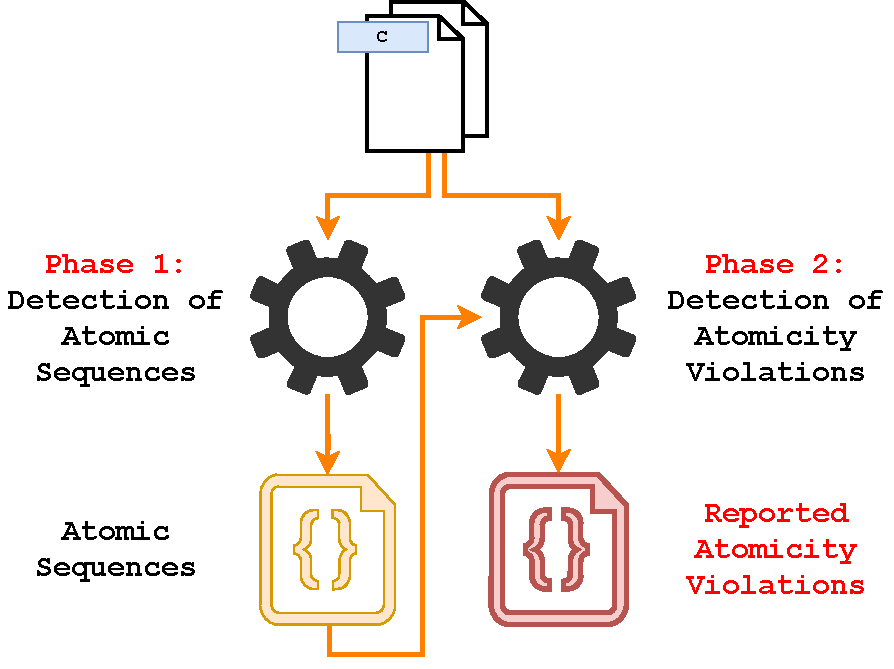
\includegraphics[width=.66 \linewidth]{analyser-proposal.pdf}
    \caption{\emph{Phases} of the analysis of the Atomer's first version and the analysis \emph{high-level process} illustration~\cite{harmimBP}}
    \label{fig:atomerPhasesSequences}
\end{figure}

This section provides a~high-level view of the \emph{abstract interpretation} underlying Atomer. The concrete types of the \emph{abstract states} (i.e., elements of the \emph{abstract domain}~$ Q $) and the \emph{summaries}~$ \chi $, along with the implementation of all necessary \emph{abstract interpretation operators} are stated in Chapter~4 of~\cite{harmimBP}. However, actually, the abstract states~$ s \in Q $ of both phases of the analysis are proposed as \emph{sets}. So, in fact, the \emph{ordering operator}~$ \sqsubseteq $ is implemented using testing for a~\emph{subset} (i.e., $ s \sqsubseteq s^\prime \Longleftrightarrow s \subseteq s^\prime $, where $ s, s^\prime \in Q $), the \emph{join operator}~$ \sqcup $ is implemented as the \emph{set union} (i.e., $ s \sqcup s^\prime \Longleftrightarrow s \cup s^\prime $), and the \emph{widening operator}~$ \triangledown $ is implemented using the join operator (i.e., $ s\,\triangledown\,s^\prime \Longleftrightarrow s \sqcup s^\prime $) since the domains are \emph{finite}. Furthermore, it is essential to note that the proposed analysis is neither \emph{sound} nor \emph{complete}. Its goal is to effectively find bugs rather than formally verify the absence of atomicity violations.

Function summaries are in the below sections reduced to the output parts only (\emph{post-conditions}~$ R $). The input parts of summaries (\emph{pre-conditions}~$ P $) are in case of the proposed analysis always empty because, so far, it is not necessary to have any pre-conditions for analysed functions. Thus, in this case, \emph{Hoare triples}\,---\,$ true\ S\ \{R\} $\,---\,are used, where~$ S $ is an analysed function, i.e., $ P = true $.

Listings in the below sections are pieces of programs written in the C~language (assuming \texttt{lock}/\texttt{unlock} functions for \emph{mutual exclusion} to \emph{critical sections}).

\subsection{Phase~1\,---\,Detection of Atomic Sequences}

Before detecting \emph{atomicity violations} may begin, it is required to have \emph{contracts for concurrency} introduced earlier. Phase~1 of Atomer is able to produce such contracts, i.e., it detects \emph{sequences of functions} that should be \emph{executed atomically}. Intuitively, the detection is based on looking for sequences of functions executed atomically, in particular, under some \emph{lock}, on some path through a~program. The assumption is that if it is \emph{once needed to execute a~sequence atomically}, it should probably be \emph{always executed atomically}.

For a~description of the analysis, it is first needed to introduce a~notion of a~\emph{reduced sequence} of function calls. Such a~sequence denotes a~sequence in which the \emph{first appearance} of each function is recorded only. It is needed to ensure the \emph{finiteness} of the sequences derived by the analysis, and hence the analysis's \emph{termination}. The detection of sequences of calls to be executed atomically is based on analysing all paths through the CFG of a~function and generating all pairs $ (A, B) \in \Sigma^* \times \Sigma^* $ (where~$ \Sigma $ is the set of functions of a~given program) of reduced sequences of function calls for each path such that: $ A $ is a~reduced sequence of function calls that appear between the beginning of the function being analysed and the first lock; between an unlock and a~subsequent lock; or between an unlock and the end of the function being analysed. $ B $ is a~reduced sequence of function calls that follow the calls from~$ A $, and that appear between a~lock and unlock (or between a~lock and the end of the function being analysed). Thus, the abstract states of the analysis are elements of the set~$ 2^{2^{\Sigma^* \times \Sigma^*}} $ because there is a~set of the $ (A, B) $ pairs for each program path.

It would be more precise to generate longer sequences of type $ A_1 \cdot B_1 \cdot A_2 \cdot B_2 \cdot \ldots\ $ instead of the sets of the pairs $ (A, B) $. Nevertheless, it would be more challenging to ensure the above longer sequences' finiteness and the sets of these sequences' finiteness. Moreover, there would be a~significantly larger \emph{state space explosion problem}~\cite{stateExpl}. So, the proposed representation of the sets of pairs of sequences has been chosen to compromise accuracy and efficiency. However, the experiments described in Chapter~5 of~\cite{harmimBP} show that it needs even more pronounced abstraction for appropriate \emph{scalability}.

Formally, the \emph{initial abstract state} of a~function is defined as $ s_{init} = \{\{(\varepsilon, \varepsilon)\}\} $, where~$\varepsilon $ indicates an empty sequence. To formalise the analysis of a~function, let~\texttt{f} be a~called leaf function. Further, let~$ s_\mathtt{g} $ be the abstract state of a~function~\texttt{g} being analysed before the function~\texttt{f} is called. After the call of~\texttt{f}, the abstract state will be changed as follows:
$$
\begin{multlined}
    s_\mathtt{g} = \bb{\{}p^\prime \in 2^{\Sigma^* \times \Sigma^*}\ |\ \exists\,p \in s_\mathtt{g} : p^\prime = \bA{\{} (A^\prime, B^\prime) \in \Sigma^* \times \Sigma^*\ |\ \exists\,(A, B) \in p : \\
%
    \bB{[}\neg actual(p, (A, B)) \wedge (A^\prime, B^\prime) = (A, B)\bB{]} \vee \bC{[}actual(p, (A, B)) \\
%
    \wedge \bD{[}(lock \wedge (A^\prime, B^\prime) = (A, B \cdot \mathtt{f})) \vee (\neg lock \wedge (A^\prime, B^\prime) = (A \cdot \mathtt{f}, B))%
%
    \bD{]}\bC{]}\bA{\}}\bb{\}}
\end{multlined}
$$
where $ actual $ is a~Boolean function that determines whether a~given $ (A, B) $ pair is the most recent pair of sequences of the current program state for a~given program path. Furthermore, $ lock $ is a~predicate indicating whether the current program state is inside an \emph{atomic block}. Further, let~$ s_\mathtt{g} $ be the abstract state of a~function~\texttt{g} being analysed before an unlock is called. After the unlock is called, a~new $ (A, B) $ pair is created and labelled as an actual using the function $ setActual $ as follows:
$$
\begin{multlined}
    s_\mathtt{g} = \bb{\{}p^\prime \in 2^{\Sigma^* \times \Sigma^*}\ |\ \exists\,p \in s_\mathtt{g} : p^\prime = \bA{\{}(A, B) \in \Sigma^* \times \Sigma^*\ | \\
%
    \bB{[}(A, B) = (\varepsilon, \varepsilon) \wedge setActual(p, (A, B))\bB{]} \vee (A, B) \in p%
%
    \bA{\}}\bb{\}}
\end{multlined}
$$

\begin{example}
    For an explanation of the computation of the sets of the pairs $ (A, B) $, assume that a~state of the analysis of a~program~$ S $ is the following sequence of function calls: $ \mathtt{f} \cdot \mathtt{g} $; and a~state of the analysis of a~program~$ S^\prime $ is the following sequence of function calls: $ \mathtt{f} \cdot \mathtt{g}\ [\mathtt{m} \cdot \mathtt{n} $. The square brackets are used to indicate an \emph{atomic sequence} (the closing square bracket is missing in the case of the program~$ S^\prime $, which means that the program state is currently inside an atomic block). The computed abstract state for the program~$ S $ is $ s_S = \{\{(\mathtt{f} \cdot \mathtt{g},\ \varepsilon)\}\} $, and for the program~$ S^\prime $, it is $ s_{S^\prime} = \{\{(\mathtt{f} \cdot \mathtt{g},\ \mathtt{m} \cdot \mathtt{n})\}\} $. Now, if the next instruction is a~call of a~function~\texttt{x}, in the case of the program~$ S $, the call will be added to the first~$ A $ sequence, and in the case of the program~$ S^\prime $, the call will be added to the first~$ B $ sequence as follows: $ s_S = \{\{(\mathtt{f} \cdot \mathtt{g} \cdot \mathtt{x},\ \varepsilon)\}\} $, $ s_{S^\prime} = \{\{(\mathtt{f} \cdot \mathtt{g},\ \mathtt{m} \cdot \mathtt{n} \cdot \mathtt{x})\}\} $. Subsequently, if the next step in the program~$ S $ is a~lock call, the next function calls will be added to the first~$ B $ sequence of the set~$ s_S $. And if the next step in the program~$ S^\prime $ is an unlock call, it will be created a~new element of the first set of the set~$ s_{S^\prime} $, and the next function calls will be added to the~$ A $ sequence of this element. Finally, if a~function~\texttt{y} is called, the resulting sets will look like follows: $ s_S = \{\{(\mathtt{f} \cdot \mathtt{g} \cdot \mathtt{x},\ \mathtt{y})\}\} $, $ s_{S^\prime} = \{\{(\mathtt{f} \cdot \mathtt{g},\ \mathtt{m} \cdot \mathtt{n} \cdot \mathtt{x}), (\mathtt{y},\ \varepsilon)\}\} $. Note that the final sequences of function calls look like follows: $ \mathtt{f} \cdot \mathtt{g} \cdot \mathtt{x}\ [\mathtt{y} $ and $ \mathtt{f} \cdot \mathtt{g}\ [\mathtt{m} \cdot \mathtt{n} \cdot \mathtt{x}]\ \mathtt{y} $ for the programs~$ S $ and~$ S^\prime $, respectively.
\end{example}

A~\emph{summary}~$ \chi_\mathtt{f} \in 2^{\Sigma^*} \times \Sigma^* $ of
a~function~\texttt{f} is then a~pair $ \chi_\mathtt{f} = (\mathcal{B},
C) $, where:
\begin{itemize}
    \item $ \mathcal{B} $ is a~set constructed such that it contains all the~$ B $ sequences that appear on program paths through~\texttt{f}, i.e., those computed within the $ (A, B) $ pairs at the exit of~\texttt{f}. Formally, $ \mathcal{B} = \{B^\prime \in \Sigma^*\ |\ \exists\,p \in s_\mathtt{f} : \exists\,(A, B) \in p : B \neq \varepsilon \wedge B^\prime = B\} $, where~$ s_\mathtt{f} $ is the abstract state at the end of the abstract interpretation of~\texttt{f}. In other words, this component of the summary is a~set of sequences of atomic function calls appearing in~\texttt{f}.

    \item $ C $ is a~\emph{concatenation} of all the~$ A $ and~$ B $ sequences with removed duplicates of function calls. In particular, assume that the following set of $ (A, B) $ pairs is computed at the exit of~\texttt{f}: $ \{(A_1, B_1), (A_2, B_2),\,\ldots\,, (A_n, B_n)\} $, then the result is the sequence $ A_1 \cdot B_1 \cdot A_2 \cdot B_2 \cdot \ldots \cdot A_n \cdot B_n $ with removed duplicates. Formally,
        $$
            C = reduce(\bigcup\limits_{c\,\in\,C^\prime}^\cdot c)
        $$
        where $ C^\prime = \{c \in \Sigma^*\ |\ \exists\,p \in s_\mathtt{f} : \exists\,(A, B) \in p: c = A \cdot B\} $, $ \dot\bigcup $ concatenates all sequences of a~set, and $ reduce $ is a~function that removes duplicates of function calls. Intuitively, in this component of the summary, the analysis gathers occurrences of all called functions within the analysed function obtained by a~concatenation of all the~$ A $ and~$ B $ sequences. $ C $ is recorded to facilitate the derivation of atomic call sequences that show up higher in the \emph{call hierarchy}. Indeed, while locks/unlocks can appear in such a~\emph{higher-level} function, parts of the call sequences can appear lower in the call hierarchy.
\end{itemize}

\begin{example}
    For instance, the analysis of the function~\texttt{f} from Listing~\ref{list:atomerPhase1} produces the following sequences:
    $$
        \overbrace{\mathtt{x} \cdot \text{\texttt{\sout{x}}} \cdot \mathtt{y}}^{A_1} \overbrace{[\mathtt{a} \cdot \mathtt{b} \cdot \text{\texttt{\sout{b}}}]}^{B_1}
        \overbrace{\mathtt{y} \cdot \text{\texttt{\sout{y}}}}^{A_2} \overbrace{[\mathtt{a} \cdot \mathtt{c}]}^{B_2}
        \text{\sout{\ensuremath{\overbrace{\mathtt{y}}^{A_3} \overbrace{[\mathtt{a} \cdot \mathtt{a} \cdot \mathtt{c}]}^{B_3}}}}
    $$
    The functions~\texttt{a}, \texttt{b}, \texttt{c}, \texttt{x}, \texttt{y} are not deeper analysed because it is assumed that these functions are leaf nodes of the call graph. The strikethrough of the functions~\texttt{b}, \texttt{x}, \texttt{y} denotes removing already recorded function calls in the~$ A $ and~$ B $ sequences to get the reduced form. The strikethrough of the entire sequence $ \mathtt{y}\ [\mathtt{a} \cdot \mathtt{a} \cdot \mathtt{c}] $ means discarding sequence already seen before. For the above, the abstract state at the end of the abstract interpretation of the function~\texttt{f} is $ s_\mathtt{f} = \{\{(\mathtt{x} \cdot \mathtt{y},\ \mathtt{a} \cdot \mathtt{b}), (\mathtt{y},\ \mathtt{a} \cdot \mathtt{c}), (\varepsilon,\ \varepsilon)\}\} $. The derived summary~$ \chi_\mathtt{f} $ for the function~\texttt{f} is $ \chi_\mathtt{f} = (\mathcal{B}, C) $, where $ \mathcal{B} = \{\mathtt{a} \cdot \mathtt{b},\ \mathtt{a} \cdot \mathtt{c}\} $, i.e., $ B_1 $ and~$ B_2 $; and $ C = \mathtt{x} \cdot \mathtt{y} \cdot \mathtt{a} \cdot \mathtt{b} \cdot \mathtt{c} $, i.e., the concatenation of~$ A_1 $, $ B_1 $, $ A_2 $, $ B_2 $ from which duplicate function calls were removed.
\end{example}

%~-
\begin{lstlisting}[style=c, label={list:atomerPhase1}, float=hbt, caption={A~code snippet used for an illustration of the derivation of \emph{sequences of functions called atomically}}]
void f()
{
    x(); x(); y();
    <@\red{lock}@>(&L); // a . b
    a(); b(); b();
    <@\red{unlock}@>(&L);
    y(); y();
    <@\red{lock}@>(&L); // a . c
    a(); c();
    <@\red{unlock}@>(&L);
    y();
    <@\red{lock}@>(&L); // a . c
    a(); a(); c();
    <@\red{unlock}@>(&L);
}
\end{lstlisting}
%~+

Further, it is demonstrated how the results of the analysis of \emph{nested functions} are used during the detection of atomic sequences. The result of the analysis of a~nested function is used as follows. When calling an already analysed function, one plugs the sequence from the second component of its summary (i.e., the~$ C $ sequence) into the most recent~$ A $ or~$ B $ sequence of all the program paths (where a~program path corresponds to a~single element of an abstract state, i.e., a~set of the $ (A, B) $ pairs). In particular, assume that $ (A, B) $ is the most recent pair of sequences of the program state of a~path being analysed. Subsequently, it is called a~function~\texttt{f} with a~non-empty summary (i.e., $ C \neq \varepsilon $). If the current program state of the analysed function is inside an atomic block, the analysis in this step will transform the pair~$ (A, B) $ to a~new $ (A^\prime, B^\prime) $ pair as follows: $ (A^\prime, B^\prime) = (A, B \cdot \mathtt{f} \cdot C) $. Otherwise, $ (A^\prime, B^\prime) = (A \cdot \mathtt{f} \cdot C, B) $. In such cases where a~summary is empty, i.e., there are no function calls in a~called function, or it is a~leaf node of the call graph, just the function name is appended to the most recent~$ A $ or~$ B $ sequences of all the program paths. To formalise this process, let~\texttt{f} be a~called function that was already analysed, and the second component of its summary is~$ C $. Further, let~$ s_\mathtt{g} $ be the abstract state of a~function~\texttt{g} being analysed before the function~\texttt{f} is called. After the call of~\texttt{f}, the abstract state will be changed as follows:
$$
\begin{multlined}
    s_\mathtt{g} = \bb{\{}p^\prime \in 2^{\Sigma^* \times \Sigma^*}\ |\ \exists\,p \in s_\mathtt{g} : p^\prime = \bA{\{}(A^\prime, B^\prime) \in \Sigma^* \times \Sigma^*\ |\ \exists\,(A, B) \in p : \\
%
    \bB{[}\neg actual(p, (A, B)) \wedge (A^\prime, B^\prime) = (A, B)\bB{]} \vee \bC{[}actual(p, (A, B)) \\
%
    \wedge \bD{[}(lock \wedge (A^\prime, B^\prime) = (A, B \cdot \mathtt{f} \cdot C)) \vee (\neg lock \wedge (A^\prime, B^\prime) = (A \cdot \mathtt{f} \cdot C, B))%
%
    \bD{]}\bC{]}\bA{\}}\bb{\}}
\end{multlined}
$$

\begin{example}
    This example shows how the function~\texttt{g} from Listing~\ref{list:atomerPhase1Nested} would be analysed using the result of the analysis of the function~\texttt{f} from Listing~\ref{list:atomerPhase1}. The second component of~$ \chi_\mathtt{f} $ is $ C = \mathtt{x} \cdot \mathtt{y} \cdot \mathtt{a} \cdot \mathtt{b} \cdot \mathtt{c} $. The analysis of the function~\texttt{g} produces the following sequence:
    $$
        \mathtt{x} \cdot \mathtt{f} \cdot \text{\texttt{\sout{x}}} \cdot \mathtt{y} \cdot \mathtt{a} \cdot \mathtt{b} \cdot \mathtt{c} \cdot \mathtt{z}\ [\mathtt{f} \cdot \mathtt{x} \cdot \mathtt{y} \cdot \mathtt{a} \cdot \mathtt{b} \cdot \mathtt{c}]
    $$
    For the above, the abstract state at the end of the abstract interpretation of the function~\texttt{g} is $ s_\mathtt{g} = \{\{(\mathtt{x} \cdot \mathtt{f} \cdot \mathtt{y} \cdot \mathtt{a} \cdot \mathtt{b} \cdot \mathtt{c} \cdot \mathtt{z},\ \mathtt{f} \cdot \mathtt{x} \cdot \mathtt{y} \cdot \mathtt{a} \cdot \mathtt{b} \cdot \mathtt{c} \cdot), (\varepsilon,\ \varepsilon)\}\} $. The derived summary~$ \chi_\mathtt{g} $ for the function~\texttt{g} is $ \chi_\mathtt{g} = (\{\mathtt{f} \cdot \mathtt{x} \cdot \mathtt{y} \cdot \mathtt{a} \cdot \mathtt{b} \cdot \mathtt{c} \cdot\},\ \mathtt{x} \cdot \mathtt{f} \cdot \mathtt{y} \cdot \mathtt{a} \cdot \mathtt{b} \cdot \mathtt{c} \cdot \mathtt{z}) $.
\end{example}

%~-
\begin{lstlisting}[style=c, label={list:atomerPhase1Nested}, float=hbt, caption={A~code snippet used to illustrate the derivation of sequences of functions called atomically with a~\emph{nested function call} (function~\texttt{f} is defined in Listing~\ref{list:atomerPhase1})}]
void g()
{
    x(); f(); z();
    <@\red{lock}@>(&L); // f . x . y . a . b . c
    f();
    <@\red{unlock}@>(&L);
}
\end{lstlisting}
%~+

\subsubsection{Cases Where Lock/Unlock Calls Are Not Paired in a~Function}

For treating cases where \emph{lock/unlock calls are not paired} in a~function\,---\,as demonstrated in Listing~\ref{list:AtomerPhase1NotPairedLock}\,---\,the following solution is implemented in the basic version of Atomer.

\emph{Everything is unlocked at the end} of a~function, i.e., one \emph{virtually appends} an unlock to the end of the function if it is necessary. Then, for the function~\texttt{m} from Listing~\ref{list:AtomerPhase1NotPairedLock}, the atomic section is virtually closed. Hence, there is detected an atomic sequence $ \mathtt{a} $. In particular, the summary is as follows: $ \chi_\mathtt{m} = (\{\mathtt{a}\},\ \mathtt{a}) $.

Moreover, \emph{all unlock calls not preceded by a~lock are ignored}. Thus, in the function~\texttt{n} from Listing~\ref{list:AtomerPhase1NotPairedLock}, there are not detected any atomic sequences: $ \chi_\mathtt{n} = (\emptyset,\ \mathtt{a}) $.

%~-
\begin{lstlisting}[style=c, label={list:AtomerPhase1NotPairedLock}, float=hbt, caption={A~code snippet used to illustrate treating cases where \emph{lock/unlock calls are not paired} in a~function}]
void m()
{
    <@\red{lock}@>(&L); // a
    a();
}
void n()
{
    a();
    <@\red{unlock}@>(&L);
}
\end{lstlisting}
%~+

\paragraph{Summary of Phase~1}
The derived sequences of calls assumed to execute atomically\,---\,the~$ \mathcal{B} $ sequences\,---\,from the summaries of all analysed functions are stored into a~file used during Phase~2, which is described later on.

\subsection{Phase~2\,---\,Detection of Atomicity Violations}

In the second phase of the analysis, i.e., when \emph{detecting violations} of the atomic sequences obtained from Phase~1, the analysis looks for \emph{pairs of functions} that \emph{should be called atomically} (or just for single functions if there is only one function call in an atomic sequence) and that are not executed atomically (i.e., under a~lock) on some path through the CFG. The pairs of function calls to be checked for atomicity are obtained as follows. For each function~\texttt{f} with a~Phase~1 summary~$ \chi_\mathtt{f} = (\mathcal{B}, C) $ in a~given program~$ S $, where $ \mathcal{B} = \{B_1, B_2,\ \ldots\ , B_n\} $, the analysis considers \emph{every pair} $ (\mathtt{x}, \mathtt{y}) \in \Sigma \times \Sigma $ of functions that appear as a~\emph{substring} in some of the~$ B_i $ sequences, i.e., $ B_i = w \cdot \mathtt{x} \cdot \mathtt{y} \cdot w^\prime $ for some sequences~$ w, w^\prime $. Note that~\texttt{x} could be~$ \varepsilon $ (an empty sequence) if some~$ B_i $ consists of a~single function. All these \uv{atomic pairs} are put into the set $ \Omega \in 2^{\Sigma \times \Sigma} $. More formally,
$$
\begin{multlined}
    \Omega = \bb{\{}(\mathtt{x}, \mathtt{y}) \in \Sigma \times \Sigma\ |\ \exists\,(\mathcal{B}, C) \in X_S : \exists\,B \in \mathcal{B} : \bA{[}|B| = 1 \wedge (\mathtt{x}, \mathtt{y}) = (\varepsilon, B)\bA{]} \\
%
    \vee \bB{[}|B| > 1 \wedge \exists\,w, w^\prime \in \Sigma^* : B = w \cdot \mathtt{x} \cdot \mathtt{y} \cdot w^\prime \wedge (\mathtt{x}, \mathtt{y}) \neq (\varepsilon, \varepsilon)%
%
    \bB{]}\bb{\}}
\end{multlined}
$$
where~$ X_S \in 2^{2^{\Sigma^*} \times \Sigma^*} $ is a~set of all Phase~1 summaries of the program~$ S $.

\begin{example}
    For instance, assume that in Phase~1, there was analysed a~function~\texttt{f}. It produced the summary $ \chi_\mathtt{f} = (\mathcal{B}, C) $, where $ \mathcal{B} = \{\mathtt{a} \cdot \mathtt{b} \cdot \mathtt{c},\ \mathtt{a} \cdot \mathtt{c} \cdot \mathtt{d}\} $, i.e., a~set of sequences of functions that should be called atomically. The analysis will then look for the following pairs of functions that are not called atomically: $ \Omega = \{\mathtt{a} \cdot \mathtt{b},\ \mathtt{b} \cdot \mathtt{c},\ \mathtt{a} \cdot \mathtt{c},\ \mathtt{c} \cdot \mathtt{d}\} $.
\end{example}

An element of this phase's abstract state is a~triple $ (\mathtt{x}, \mathtt{y}, \delta) \in \Sigma \times \Sigma \times 2^{\Sigma \times \Sigma \times \mathbb{N}} $ where $ (\mathtt{x}, \mathtt{y}) $ is a~pair of the most recent calls of functions performed on the program path being explored, and~$ \delta $ is a~set of so far detected \emph{pairs that violate atomicity} on particular lines of code. Thus, the abstract states are elements of the set~$ 2^{\Sigma \times \Sigma \times 2^{\Sigma \times \Sigma \times \mathbb{N}}} $. Whenever a~function~\texttt{f} is called on some path that led to an abstract state $ (\mathtt{x}, \mathtt{y}, \delta) $, a~new pair $ (\mathtt{x}^\prime, \mathtt{y}^\prime) $ of the most recent function calls is created from the previous pair $ (\mathtt{x}, \mathtt{y}) $ such that $ (\mathtt{x}^\prime, \mathtt{y}^\prime) = (\mathtt{y}, \mathtt{f}) $. Further, when the current program state is not inside an atomic block, the analysis checks whether the new pair (or just the last call) violates atomicity (i.e., $ (\mathtt{x}^\prime, \mathtt{y}^\prime) \in \Omega \vee (\varepsilon, \mathtt{y}^\prime) \in \Omega $). When it does, it is added to the set~$ \delta $ of pairs that violate atomicity.

Formally, the initial abstract state (in this phase) of a~function is defined as $ s_{init} = \{(\varepsilon, \varepsilon, \emptyset)\} $. To formalise the analysis of a~function, let~\texttt{f} be a~called leaf function on a~line~$ c $. Further, let~$ s_\mathtt{g} $ be the abstract state of a~function~\texttt{g} being analysed before the function~\texttt{f} is called. After the call of~\texttt{f}, the abstract state will be changed as follows:
$$
\begin{multlined}
    s_\mathtt{g} = \bb{\{}(\mathtt{x}^\prime, \mathtt{y}^\prime, \delta^\prime) \in \Sigma \times \Sigma \times 2^{\Sigma \times \Sigma \times \mathbb{N}}\ |\ \exists\,(\mathtt{x}, \mathtt{y}, \delta) \in s_\mathtt{g} : (\mathtt{x}^\prime, \mathtt{y}^\prime) = (\mathtt{y}, \mathtt{f}) \\
%
    \wedge \bA{[}\bB{(}\neg lock \wedge \delta^\prime = \bC{\{}(\mathtt{x}^{\prime\prime}, \mathtt{y}^{\prime\prime}, c^\prime) \in \Sigma \times \Sigma \times \mathbb{N}\ |\ (\mathtt{x}^{\prime\prime}, \mathtt{y}^{\prime\prime}, c^\prime) \in \delta \\
%
    \vee [\bD{(}(\mathtt{x}^{\prime\prime}, \mathtt{y}^{\prime\prime}) = (\mathtt{x}^{\prime}, \mathtt{y}^\prime) \vee (\mathtt{x}^{\prime\prime}, \mathtt{y}^{\prime\prime}) = (\varepsilon, \mathtt{y}^\prime)\bD{)} \wedge (\mathtt{x}^{\prime\prime}, \mathtt{y}^{\prime\prime}) \in \Omega \wedge c^\prime = c]\bC{\}}\bB{)} \vee (lock \wedge \delta^\prime = \delta)%
%
    \bA{]}\bb{\}}
\end{multlined}
$$

A~\emph{summary} of the second phase of the analysis\,---\,$ \chi_\mathtt{f} \in 2^{\Sigma \times \Sigma \times \mathbb{N}} $\,---\,of a~function~\texttt{f} is then $ \chi_\mathtt{f} = \Delta $, where~$ \Delta $ is a~set of pairs that violate atomicity within the function~\texttt{f}. $ \Delta $ is constructed such that it contains a~union of all the~$ \delta $ sets that appear on program paths through~\texttt{f}. Formally, $ \Delta = \bigcup_{\delta^\prime\,\in\,\Delta^\prime} \delta^\prime $, where $ \Delta^\prime = \{\delta^\prime \in 2^{\Sigma \times \Sigma \times \mathbb{N}}\ |\ \exists\,p \in s_\mathtt{f} : \exists\,(\mathtt{x}, \mathtt{y}, \delta) \in p : \delta \neq \emptyset \wedge \delta^\prime = \delta\} $ and~$ s_\mathtt{f} $ is the abstract state at the end of the abstract interpretation of~\texttt{f}.

The analysis of functions with \emph{nested function calls} and cases where \emph{lock/unlock calls are not paired} within functions are handled analogically as in Phase~1. For a~detailed explanation, see~\cite{harmimBP}.

\begin{example}
    To demonstrate the detection of an atomicity violation, assume the functions~\texttt{f} and~\texttt{g} from Listing~\ref{list:AtomerPhase2}. The set of atomic sequences of the function~\texttt{f} with the first phase's summary~$ \chi_\mathtt{f} = (\mathcal{B}, C) $ is $ \mathcal{B} = \{\mathtt{a} \cdot \mathtt{b} \cdot \mathtt{c}\} $, thus, $ \Omega = \{(\mathtt{a}, \mathtt{b}), (\mathtt{b}, \mathtt{c})\} $. In the function~\texttt{g}, an atomicity violation is detected because the pair of functions~\texttt{b}, \texttt{c} is not called atomically on line~12, i.e., $ (\mathtt{b}, \mathtt{c}) \in \Omega $. Consequently, the derived summary~$ \chi_\mathtt{g} $ for the function~\texttt{g} for the second phase of the analysis is $ \chi_\mathtt{g} = \{(\mathtt{b}, \mathtt{c}, 12)\} $.
\end{example}

%~-
\begin{lstlisting}[style=c, label={list:AtomerPhase2}, float=hbt, caption={An example of an \emph{atomicity violation}}]
void f()
{
    x();
    <@\red{lock}@>(&L); // a . b . c
    a(); b(); c();
    <@\red{unlock}@>(&L);
    y();
}
void g()
{
    x();
    b(); c(); // <@\red{ATOMICITY\_VIOLATION:}@> (b, c)
    y();
}
\end{lstlisting}
%~+

\paragraph{Summary of Phase~2}
The sets of pairs that violate atomicity\,---\,the~$ \Delta $ sets\,---\,from the summaries of all analysed functions are finally reported to the user.


\section{Atomer's Limitations}
\label{sec:atomerLimits}

The basic version of Atomer has been proposed as it is detailed in Section~\ref{sec:atomerDesing}. The first version of the analyser has also been implemented in~\cite{harmimBP}, and it works as expected. Moreover, it can be used in practice to analyse various kinds of programs, and it may find \emph{real-world atomicity related bugs}. Nevertheless, there are still several \emph{limitations} and cases where the original version of Atomer would not work correctly, i.e., cases not addressed during the original proposal. Some of these cases are briefly discussed already in~\cite{harmimBP} and further described in~\cite{excel2021Harmim}.

So far, Atomer does not distinguish \emph{different lock instances} used simultaneously in a~program. Only calls of locks/unlocks are identified, and the parameters of these calls\,---\,\emph{lock objects}\,---\,are not considered at all. Therefore, if there are several lock objects used, the analysis does not work correctly. Although this may happen in \emph{real-life programs}, insomuch as one could have, e.g., another (smaller) atomic section inside a~current atomic section (this does not have to be evident at first because the \emph{inner atomic section} could be, e.g., inside a~nested function). For example,
$$
    \mathtt{\ldots\ lock(L1);\ \ldots\ lock(L2);\ \ldots\ unlock(L2);\ \ldots\ unlock(L1);\ \ldots}
$$
Another possibility is an \emph{alternating sequence of locks}, e.g., two locks are locked at first, and then, they are unlocked in the same order, i.e.,
$$
    \mathtt{\ldots\ lock(L1);\ \ldots\ lock(L2);\ \ldots\ unlock(L1);\ \ldots\ unlock(L2);\ \ldots}
$$

Another limitation of Atomer's basic version is that it supports only the analysis of programs written in the \emph{C~language} that use \emph{PThread} locks to \emph{synchronise concurrent threads}. Of course, in practice, many other \emph{types of locks} for synchronisation of concurrent threads or even synchronisation of \emph{concurrent processes} are used. Although the first version of Atomer can analyse C~programs with other types of locks, these locks are not recognised as locks. Thus, the analysis would not work as expected. It would definitely be helpful also to analyse other languages than just~C. As described in Section~\ref{sec:fbinfer}, Facebook Infer is capable of analysing programs written in~C, C++, Objective-C, Java, and C\#. The analysis algorithm could then be the same for all these languages because Facebook Infer's \emph{intermediate language} is analysed instead of directly analysing the input languages. Again, the first version of Atomer should be able to analyse the above languages, but it has not been tested within~\cite{harmimBP}. However, most importantly, other languages may use \emph{very different lock types}, which would not be recognised. Examples of some advanced locking mechanisms (not supported by the basic version of Atomer) are \emph{lock guards}, \emph{re-entrant locks}, or \emph{try-locks}.

Regarding \emph{scalability}, the basic version of Atomer can have problems with more \emph{extensive} and \emph{complex} programs, as mentioned in~\cite{harmimBP} (problems with \emph{memory} as well as problems with the \emph{analysis time}). The problem is working with the sets of $ (A, B) $ pairs of \emph{sequences} in the abstract states of Phase~1 and working with \emph{sequences} of calls in the summaries of this phase. It may be necessary to store many of these sequences, and they can be very long (due to all different paths through the CFG of an analysed program). It may lead to the \emph{state space explosion problem}~\cite{stateExpl}.

One of the main reasons that Atomer's first version reports \emph{false alarms} is that in \emph{critical sections}, in real-world programs, there are sometimes called \emph{generic functions} that do not influence atomicity violations (such as functions for printing to the standard output, functions for recasting variables to different types, functions related to iterators, and whatever other \uv{safe} functions for particular program types). Often, to find some atomicity violations, it is sufficient to focus only on certain \uv{critical} functions. In practice, another issue is that in an analysed program, there can be \uv{large} critical sections or critical sections in which appear function calls with a~\emph{deep hierarchy of nested function calls}. All the above cases may cause massive and \uv{imprecise} atomic sequences that are the source of false alarms. However, regardless of the above issues, Atomer can still report quite some false alarms. It is due to the assumption that \emph{sequences called atomically once} should \emph{always be called atomically}, but this does not always have to hold. None of the above reasons that can generate false alarms is resolved in the first version of Atomer.

The next source of false alarms is something that the author of this work calls \emph{local atomicity violations}. Imagine a~function~\texttt{f} that contains non-atomic calls of functions~\texttt{a}, \texttt{b}, and these functions should always be invoked atomically. Obviously, this is an atomicity violation. However, suppose that~\texttt{f} is called exclusively from atomic sections of other functions higher in the call hierarchy. In this case, in effect, that is not a~real atomicity violation (it can be considered as a~local atomicity violation within a~single function, but globally, it is not). As a~consequence, a~false alarm would be reported by the basic version of Atomer. In real-life programs, this situation may be fairly common due to \emph{complicated call graphs}.

Atomer considers only the \emph{basic contracts for concurrency}, defined in Section~\ref{sec:contractsBasic}. It is pretty limited in some circumstances, and therefore, Atomer can report \emph{false alarms}. The basic contracts do not take into consideration the \emph{data flow} within function calls. However, a~better idea is to work with the assumption that a~sequence of function calls must be atomic only if it \emph{handles the same data}. Assume that functions~\texttt{f}, \texttt{g} are manipulating with the same container~\texttt{C} as follows: \texttt{f(C); g(C);}. These are called atomically. Somewhere else\,---\,where~\texttt{f}, \texttt{g} are not called atomically\,---\,it does not necessarily cause an atomicity violation because they can be invoked with different arguments, which could be valid. This behaviour corresponds to the \emph{extended contracts with parameters} (see Section~\ref{sec:contractsParams}). Another (more complex) limitation is that basic contracts do not consider any \emph{contextual information}. It would be more precise to consider as atomicity violations such sequences that could be violated only by particular (\uv{dangerous}) function calls, not by any calls. For example, suppose that there is the following sequence of functions called atomically: \texttt{f(); g();}. While somewhere else, these functions are not called atomically, it does not necessarily cause that it is an atomicity violation because, in this particular context, none of the \uv{dangerous} functions can be executed by any concurrent thread. The \emph{extended contracts with spoilers} formally describe these scenarios in Section~\ref{sec:contractsSpoilers}.

A~remarkable problem (though it is not directly a~problem of Atomer) is identifying whether a~reported atomicity violation is a~\emph{real bug} or whether it is just a~false alarm. It could be really challenging, especially in \emph{extensive real-life} programs.

Solutions for some of the above issues and limitations are proposed in Chapter~\ref{chap:proposal} and further implemented in a~new version of Atomer, detailed in Chapter~\ref{chap:implement}.



%===============================================================================



\chapter{Proposal of Enhancements for Atomer}
\label{chap:proposal}

In this chapter, the author proposes solutions for some of the Atomer's limitations stated in Section~\ref{sec:atomerLimits}. The solutions enhance the analysis's \emph{precision} and \emph{scalability}. In order to formally define these enhancements, the notions and symbols introduced in Section~\ref{sec:atomerDesing} are used. Some of the enhancements were briefly discussed already in~\cite{excel2021Harmim}.

Section~\ref{sec:proposalSets} proposes an optimisation of Atomer's scalability. The following Sections~\ref{sec:proposalAdvancedLocks}, \ref{sec:proposalParametr}, \ref{sec:proposalLocalGlobalViols} cover precision improvements, i.e., extensions of Atomer with additional features that improve its ability to cope with cases that were not supported in the first version of Atomer, and that can be seen in \emph{real-life code}. Furthermore, Chapter~\ref{chap:implement} provides an overview of the implementation of all the below improvements in a~new version of Atomer.

In the following sections, to give an intuition, there are used listings with pieces of C~programs (assuming \texttt{lock/unlock} functions for \emph{mutual exclusion} to \emph{critical sections}). In addition, there are used C++ and Java programs to illustrate the \emph{locking mechanisms} in these languages.


\section{Approximation of Sequences by Sets}
\label{sec:proposalSets}

Regarding \emph{scalability}, the basic version of Atomer can have problems with more \emph{extensive} and \emph{complex} programs, which can manifest both in its \emph{time} and \emph{memory} consumption. The problems arise primarily due to working with the sets of $ (A, B) $ pairs of \textbf{sequences} of function calls in \emph{abstract states} (during Phase~1). It may be necessary to store many of these sequences, and they could be very long (due to all different paths through the CFG of an analysed program). The author's idea is to \emph{approximate} these sets by working with sets of $ (A, B) $ pairs of \textbf{sets} of function calls. Apart from representing the abstract states of the first phase of the analysis, elements of these pairs do also appear in the first phase's \emph{summaries}, and they are then used during Phase~2 as well. Thus, it is needed to make a~certain approximation in the summaries and their subsequent usage too. The approximated phases of the analysis and their collaboration are illustrated in Figure~\ref{fig:atomerPhasesSets} (one can compare that with the illustration of the first version of Atomer in Figure~\ref{fig:atomerPhasesSequences}).

\begin{figure}[hbt]
    \centering
    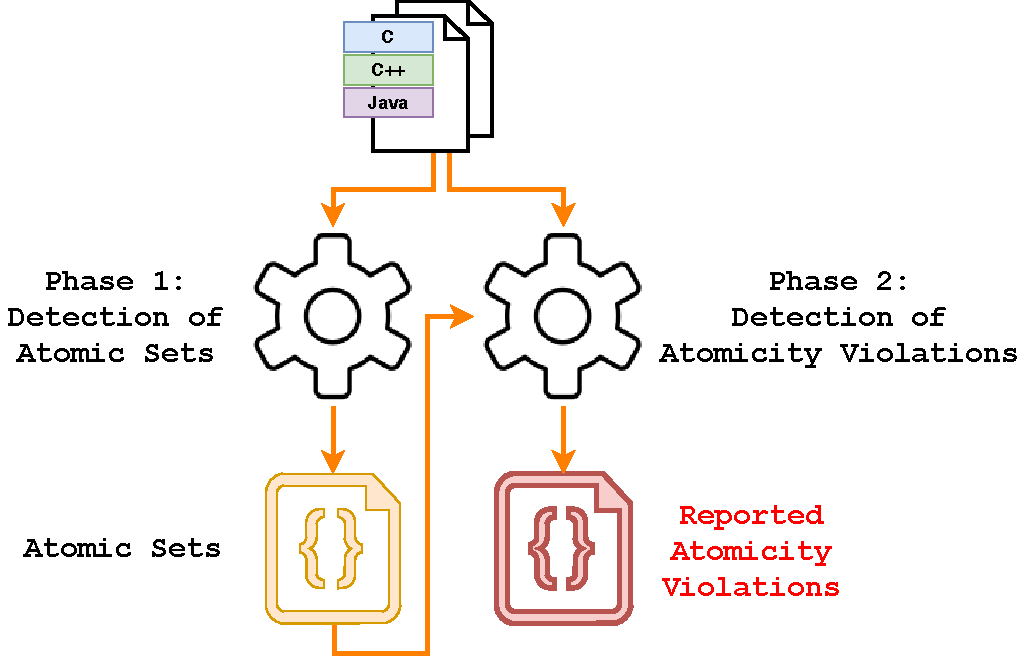
\includegraphics[width=.66 \linewidth]{analyser-proposal-sets.pdf}
    \caption{An illustration of the \emph{phases} of the Atomer's analysis and the \emph{high-level analysis process} with an \emph{approximation} of working with \emph{sequences} by working with \emph{sets} (moreover, note that a~new version of Atomer accepts programs also written in C++ and Java languages, which is described in Section~\ref{sec:implementLanguages})}
    \label{fig:atomerPhasesSets}
\end{figure}

In particular, the proposed solution is more scalable because the ordering of function calls that appear in the pairs is not relevant anymore. Therefore, less memory is required because different sequences of function calls can map the same set. The analysis is also faster since there are stored fewer sets of function calls to work with. On the other hand, the analysis is less accurate because the new approach causes some loss of information. In practice, this loss of information could eventually lead to \emph{false alarms}. However, the number of such false alarms is typically not that high as this thesis's experimental evidence shows. Moreover, later, there are discussed some techniques that may rid of these false alarms.

\subsection{Approximation with Sets in Phase~1}

The \emph{detection of sequences of calls to be executed atomically} now generates all $ (A, B) $ pairs of \textbf{sets} of function calls for each path instead of pairs of \textbf{sequences}, i.e., $ (A, B) \in 2^\Sigma \times 2^\Sigma $. Here,~$ A $, $ B $ are not \emph{reduced sequences} (the notion of a~reduced sequence is not needed anymore) but sets. The purpose of the pairs is preserved. Hence, the abstract states are elements of the set $ 2^{2^{2^\Sigma \times 2^\Sigma}} $. In all the implemented algorithms and definitions, it is sufficient to work with:
\begin{itemize}
    \item \emph{sets}~$ 2^\Sigma $ of functions, instead of \emph{sequences}~$ \Sigma^* $ of functions;

    \item the \emph{empty sets}~$ \emptyset $, instead of the \emph{empty sequences}~$ \varepsilon $; and

    \item \emph{unions}~$ \cup $ of sets, instead of the \emph{concatenation}~$ \cdot $ of sequences.
\end{itemize}

The above implies that the \emph{initial abstract state} of a~function is changed to $ s_{init} = \{\{(\emptyset, \emptyset)\}\} $. During the analysis of a~function~\texttt{g} with an abstract state~$ s_\mathtt{g} $, when a~leaf function~\texttt{f} is called, the abstract state's transformation is changed as follows:
$$
\begin{multlined}
    s_\mathtt{g} = \bb{\{}p^\prime \in 2^{2^\Sigma \times 2^\Sigma}\ |\ \exists\,p \in s_\mathtt{g} : p^\prime = \bA{\{}(A^\prime, B^\prime) \in 2^\Sigma \times 2^\Sigma\ |\ \exists\,(A, B) \in p : \\
%
    \bB{[}\neg actual(p, (A, B)) \wedge (A^\prime, B^\prime) = (A, B)\bB{]} \vee \bC{[}actual(p, (A, B)) \\
%
    \wedge \bD{[}(lock \wedge (A^\prime, B^\prime) = (A, B \cup \{\mathtt{f}\})) \vee (\neg lock \wedge (A^\prime, B^\prime) = (A \cup \{\mathtt{f}\}, B))%
%
    \bD{]}\bC{]}\bA{\}}\bb{\}}
\end{multlined}
$$
Further, when an unlock is called, a~new $ (A, B) $ pair is created as follows:
$$
\begin{multlined}
    s_\mathtt{g} = \bb{\{}p^\prime \in 2^{2^\Sigma \times 2^\Sigma}\ |\ \exists\,p \in s_\mathtt{g} : p^\prime = \bA{\{}(A, B) \in 2^\Sigma \times 2^\Sigma\ |\ \\
%
    \bB{[}(A, B) = (\emptyset, \emptyset) \wedge setActual(p, (A, B))\bB{]} \vee (A, B) \in p%
%
    \bA{\}}\bb{\}}
\end{multlined}
$$
Other algorithms (e.g., calling an already analysed \emph{nested} function) are modified analogically.

Another approximation was made in the summaries. The first component of the summary has to be changed to a~set of sets of function calls because it is constructed from the~$ B $ items from the abstract states, which are now sets. The second component of the summary can be changed to a~set of function calls because even before, it was a~reduced sequence of all the $ (A, B) $ pairs. Therefore, the ordering of function calls was significantly approximated even so. Moreover, it is used to analyse functions higher in the \emph{call hierarchy} where it is appended to~$ A $ or~$ B $, which are now sets. Thus, it would make no sense to store it in summaries as a~sequence. Formally, the form of summaries~$ \chi $ changes from $ 2^{\Sigma^*} \times \Sigma^* $ to $ 2^{2^\Sigma} \times 2^\Sigma $. In particular, a~summary~$ \chi_\mathtt{f} \in 2^{2^\Sigma} \times 2^\Sigma $ of a~function~\texttt{f} is redefined as $ \chi_\mathtt{f} = (\mathcal{B}, C) $, where:
\begin{itemize}
    \item $ \mathcal{B} = \{B^\prime \in 2^\Sigma\ |\ \exists\,p \in s_\mathtt{f} : \exists\,(A, B) \in p : B \neq \emptyset \wedge B^\prime = B\} $, where~$ s_\mathtt{f} $ is the abstract state at the end of the abstract interpretation of~\texttt{f}.

    \item $ C = \bigcup\limits_{c\,\in\,C^\prime} c $, where $ C^\prime = \{c \in 2^\Sigma\ |\ \exists\,p \in s_\mathtt{f} : \exists\,(A, B) \in p: c = A \cup B\} $.
\end{itemize}

\begin{example}
    For demonstrating the approximation of the analysis to sets, assume functions~\texttt{f} and~\texttt{g} from Listing~\ref{list:atomerPhase1Sets}. Further, assume that~\texttt{a}, \texttt{b}, \texttt{x}, \texttt{y} are leaf nodes of the call graph. Before the approximation, when the analysis was working with sequences of function calls, Phase~1 of the analysis produced the following abstract states and summaries while analysing the functions:
    \begin{itemize}
        \item $ s_\mathtt{f} = \{\{(\mathtt{x} \cdot \mathtt{y},\ \mathtt{a} \cdot \mathtt{b}), (\mathtt{y} \cdot \mathtt{x},\ \mathtt{b} \cdot \mathtt{a}), (\varepsilon,\ \varepsilon)\}\} $, $ \chi_\mathtt{f} = (\{\mathtt{a} \cdot \mathtt{b},\ \mathtt{b} \cdot \mathtt{a}\},\ \mathtt{x} \cdot \mathtt{y} \cdot \mathtt{a} \cdot \mathtt{b}) $;

        \item $ s_\mathtt{g} = \{\{(\mathtt{y} \cdot \mathtt{x},\ \mathtt{b} \cdot \mathtt{a}), (\varepsilon,\ \varepsilon)\}\} $, $ \chi_\mathtt{g} = (\{\mathtt{b} \cdot \mathtt{a}\},\ \mathtt{y} \cdot \mathtt{x} \cdot \mathtt{b} \cdot \mathtt{a}) $.
    \end{itemize}
    Whereas, after the approximation, the produced abstract states and summaries are as follows: $ s_\mathtt{f} = s_\mathtt{g} = \{\{(\{\mathtt{x}, \mathtt{y}\}, \{\mathtt{a}, \mathtt{b}\}), (\emptyset, \emptyset)\}\} $, $ \chi_\mathtt{f} = \chi_\mathtt{g} = (\{\{\mathtt{a}, \mathtt{b}\}\}, \{\mathtt{a}, \mathtt{b}, \mathtt{x}, \mathtt{y}\}) $. They are the same for both functions because there are the same locked/unlocked function calls; only the order of calls differs.
\end{example}

%~-
\begin{lstlisting}[style=c, label={list:atomerPhase1Sets}, float=hbt, caption={A~code snippet used to illustrate the proposed \emph{approximation} of the first phase of the analysis in a~new version of Atomer using \emph{sets of function calls}}]
void f()
{
    x(); y();
    <@\red{lock}@>(&L); // a . b -> {a, b}
    a(); b();
    <@\red{unlock}@>(&L);
    y(); x();
    <@\red{lock}@>(&L); // b . a -> {a, b}
    b(); a();
    <@\red{unlock}@>(&L);
}
void g()
{
    y(); x();
    <@\red{lock}@>(&L); // b . a -> {a, b}
    b(); a();
    <@\red{unlock}@>(&L);
}
\end{lstlisting}
%~+

\subsection{Approximation with Sets in Phase~2}

The \emph{detection of atomicity violations} in Phase~2 then works almost the same way as before the approximation. However, there is one difference. Before, the analysis implemented in the second phase looked for violations of atomic sequences obtained from Phase~1. Now, \textbf{atomic sets} are obtained from Phase~1; hence, the detection of atomicity violations needs to work with sets too. Again, the analysis looks for \emph{pairs of functions that should be called atomically}, while this is not the case on some path through the CFG. This algorithm is identical to the algorithm before the approximation.

Nevertheless, it is needed to propose a~new algorithm that derives the pairs of function calls (from the atomic sets) to be checked for atomicity (i.e., the set~$ \Omega \in 2^{\Sigma \times \Sigma} $). Intuitively, the second phase of the analysis now looks for non-atomic execution of any pair of functions~\texttt{f}, \texttt{g} such that $ \{\mathtt{f}, \mathtt{g}\} $ is a~\emph{subset} of some set of functions that were found to be executed atomically. In order to obtain the pairs, all possible pairs of functions are taken from atomic sets from Phase~1, i.e., all \emph{2-element variations}. Formally, let~$ S $ be an analysed program, and let $ X_S \in 2^{2^{2^\Sigma} \times 2^\Sigma} $ be a~set of all summaries of the program~$ S $. Then, all the atomic pairs (the first item of a~pair may be empty if an atomic set consists of a~single function) are obtained as follows:
$$
\begin{multlined}
    \Omega = \bb{\{}(\mathtt{x}, \mathtt{y}) \in \Sigma \times \Sigma\ |\ \exists\,(\mathcal{B}, C) \in X_S : \exists\,B \in \mathcal{B} : \bA{[}|B| = 1 \wedge (\mathtt{x}, \mathtt{y}) \in \{\varepsilon\} \times B\bA{]} \\
%
    \vee \bB{[}|B| > 1 \wedge (\mathtt{x}, \mathtt{y}) \in B \times B \wedge \mathtt{x} \neq \mathtt{y}%
%
    \bB{]}\bb{\}}
\end{multlined}
$$

\begin{example}
    For example, assume that Phase~1 analysed a~function~\texttt{f}, which produced the summary $ \chi_\mathtt{f} = (\mathcal{B}, C) $. Assume that before the approximation, a~set of sequences of functions that should be called atomically was as follows: $ \mathcal{B} = \{\mathtt{a} \cdot \mathtt{b} \cdot \mathtt{c}\} $. Then, the analysis looked for the following pairs of functions that are not called atomically: $ \Omega = \{(\mathtt{a}, \mathtt{b}), (\mathtt{b}, \mathtt{c})\} $. Since the result of the first component of the summary was changed to the set~$ \mathcal{B} $ of sets of functions that should be called atomically as follows: $ \mathcal{B} = \{\{\mathtt{a}, \mathtt{b}, \mathtt{c}\}\} $, the analysis now looks for the following pairs of functions that are not called atomically (all 2-element variations): $ \Omega = \{(\mathtt{a}, \mathtt{b}), (\mathtt{a}, \mathtt{c}), (\mathtt{b}, \mathtt{a}), (\mathtt{b}, \mathtt{c}), (\mathtt{c}, \mathtt{a}), (\mathtt{c}, \mathtt{b})\} $.
\end{example}


\section{Advanced Manipulation with Locks}
\label{sec:proposalAdvancedLocks}

The original version of Atomer does not distinguish \emph{different lock instances} in a~program. Only calls of locks/unlocks are identified, and the parameters of these calls\,---\,\emph{lock objects}\,---\,are not considered. Thus, if there are several lock objects used, the analysis does not work correctly.

In order to consider lock objects, it was proposed to distinguish between them using Facebook Infer's built-in mechanism called \emph{access paths}~\cite{accessPath}, explained below. The analyser does not perform a~classical \emph{alias analysis}, i.e., it does not perform a~precise analysis for saying when arbitrary pairs of accesses to lock objects may alias (such an analysis is considered too expensive).

\paragraph{Access Paths}
The \emph{syntactic access paths}~\cite{accessPath} represent \emph{heap locations} via the paths used to access them, i.e., they have the form of an expression consisting of a~base variable followed by a~sequence of fields. More formally, let $ Var $ be a~set of all variables that can occur in a~given program. Let $ Field $ be a~set of all possible field names that can be used in the program (e.g., structure fields). An access path~$ \pi $ from the set~$ \Pi $ of all access paths is then defined as follows:
$$
    \pi \in \Pi \Coloneqq Var \times Field^*
$$
Access paths are already implemented in Facebook Infer. For instance, the principle of using access paths is used in an existing analyser in Facebook Infer\,---\,RacerD~\cite{racerD, racerDOnline, staticRaceDetectorTruePositives}\,---\,for data race detection. In general, no sufficiently precise \emph{alias analysis} works \emph{compositionally} and \emph{at scale}. That is the motivation for using access paths in Facebook Infer.

Given a~pair of accesses to lock objects, to determine whether these locks are equal, it is needed to answer the following question: \uv{Can the accesses touch the same address?}. Remarkably, according to the authors of~\cite{racerD}, access paths alone \emph{almost} convey enough semantic information to answer the above question on their own. If two access paths are syntactically equal, it is almost (but not quite) true that they must refer to the same address. Syntactically identical paths can refer to different addresses if
\begin{enuminline}
    \item they refer to different instances of the same object, or

    \item a~prefix of the path is reassigned along one execution trace but not the other.
\end{enuminline}
These conditions cannot hold if an access path is \emph{stable}, i.e., if none of its proper prefixes appears in assignments during a~given execution trace, then it touches the same memory as all other stable accesses to the syntactic path. Therefore, the access paths' syntactic equality is a~reasonably efficient way to say (in an \emph{under-approximate fashion}) that heap access touches the same address. Also, by using access paths, RacerD detected many errors in real-world programs, proving that the use of access paths can reveal real errors. This is why it was decided to use this principle to represent locks in Atomer.

During the analysis performed by Atomer (in both phases), each atomic section is identified by an access path of the lock that guards the section; see Sections~\ref{sec:proposalMultiLocksPhase1}, \ref{sec:proposalMultiLocksPhase2}. Because \emph{syntactically identical access paths} are used as the means for distinguishing atomic sections, some atomicity violations could be missed (or some false alarms could be reported) due to distinct access paths that refer to the same memory. However, the analysis's precision is still significantly improved this way while preserving its \emph{scalability}, and the stress is anyway put on finding likely violations, not on being \emph{sound}.

Another limitation of Atomer in its basic version is that it does not count with \emph{re-entrant locks} when a~process can lock the same object multiple times without blocking itself, and then it should unlock the lock object the same number of times. This approach is, in fact, widespread, e.g., in Java, where so-called \emph{synchronised blocks} are used, as demonstrates Listing~\ref{list:reentrantJava}. These blocks are re-entrant by default. To consider re-entrant locks in the analysis, the number of locks of individual lock objects is tracked in the abstract states of both phases of the analysis. A~lock is unlocked as soon as this number decreases to~0. Also, an input parameter $ t \in \mathbb{N} $ was proposed to limit the \emph{upper bound} to which the analysis tracks precisely the number of times a~given lock is locked. When this bound is reached, the \emph{widening operator} is used to abstract the number to any value bigger than the bound. This is to ensure \emph{termination} of the analysis. The idea of this upper bound limit comes from the approach used in RacerD.

\begin{lstlisting}[style=java, label={list:reentrantJava}, float=hbt, caption={An example of \emph{re-entrant locks} in Java using the \texttt{synchronized} keyword, which is implemented as a~\emph{monitor}. In the example, there are three locks used simultaneously over the same object. The entire method~\texttt{f} is synchronised, which implicitly uses \texttt{this} as a~\emph{lock object}. Furthermore, the two \emph{synchronised blocks} explicitly use the lock object \texttt{this}}]
public synchronized void f() {
    x();
    synchronized (this) {
        a();
        synchronized (this) { b(); c(); }
        d();
    }
    y();
}
\end{lstlisting}

\subsection{Advanced Manipulation with Locks in Phase~1}
\label{sec:proposalMultiLocksPhase1}

Recall that the \emph{detection of sets of calls to be executed atomically} is based on generating the pairs $ (A, B) \in 2^\Sigma \times 2^\Sigma $. Now, these pairs are to be extended to store the access paths and the number of locks of lock objects that guard calls executed atomically, i.e., the~$ B $ sets. Therefore, the $ (A, B) $ pairs are extended to tuples $ (A, B, \pi, l) \in 2^\Sigma \times 2^\Sigma \times \Pi \times \mathbb{N}^\top $ where~$ \pi $ is an access path that identifies a~lock object that locks the atomic section that contains the calls from~$ B $, and~$ l $ is the number of locks of the lock identified by~$ \pi $. For the clarity of the below description, let~$ \pi $ be just a~base variable, i.e., $ \pi \in \Pi \Coloneqq Var \cup \{\varepsilon\} $. Note that~$ \pi $ could also be~$ \varepsilon $, which is a~special case when there is no lock associated with the~$ (A, B) $ pair so far, i.e., $ B $ is empty and a~lock was not called yet. $ \mathbb{N}^\top $ denotes $ \mathbb{N} \cup \{\top\} $, where~$ \top $ represents a~number larger than~$ t $. Thus, the \emph{abstract states} are elements of the set $ 2^{2^{2^\Sigma \times 2^\Sigma \times \Pi \times \mathbb{N}^\top}} $.

The analysis works as follows. When a~function is called, it is appended to the~$ A $ set of the element without an associated lock, i.e., the element where $ \pi = \varepsilon $. Besides, the function is appended to the~$ B $ sets of all the elements that have associated some lock that is currently locked, i.e., $ \pi \neq \varepsilon $ and $ l > 0 $. When a~lock is called, its identifier~$ \pi_i $ is associated with the element without any lock associated with it, and the counter~$ l $ of this element is set to 1. Then, $ l $ is incremented in all the elements where $ \pi = \pi_i $ and $ l > 0 $. Moreover, it is created a~new empty element without a~lock. Finally, when an unlock with the identifier~$ \pi_i $ is called, $ l $ is decremented in all the elements where $ \pi = \pi_i $ and $ l > 0 $. To formalise this process, let $ inc_\top : \mathbb{N}^\top\!\rightarrow \mathbb{N}^\top $ and $ dec_\top : \mathbb{N}^\top\!\rightarrow \mathbb{N}^\top $ be functions for incrementing and decrementing the number of locks of some lock objects w.r.t. the upper bound~$ \top $, respectively. These functions are defined as follows:
\begin{gather*}
    inc_\top(l) =
    \begin{cases}
        l + 1 & \text{for}\ l \neq \top\ \text{and}\ l + 1 < t \\
        \top & \text{otherwise}
    \end{cases}
%
    \qquad
%
    dec_\top(l) =
    \begin{cases}
        l - 1 & \text{for}\ l \neq \top\ \text{and}\ l - 1 \geq 0 \\
        0 & \text{for}\ l = 0 \\
        t - 1 & \text{otherwise, i.e.,}\ l = \top
    \end{cases}
\end{gather*}
The \emph{initial abstract state} of a~function is changed to $ s_{init} = \{\{(\emptyset, \emptyset, \varepsilon, 0)\}\} $. During the analysis of a~function~\texttt{g} with an abstract state~$ s_\mathtt{g} $, when a~leaf function~\texttt{f} is called, the abstract state's transformation is changed as follows:
$$
\begin{multlined}
    s_\mathtt{g} = \bb{\{}p^\prime \in 2^{2^\Sigma \times 2^\Sigma \times \Pi \times \mathbb{N}^\top}\ |\ \exists\,p \in s_\mathtt{g} : p^\prime = \bA{\{} (A^\prime, B^\prime, \pi^\prime, l^\prime) \in 2^\Sigma \times 2^\Sigma \times \Pi \times \mathbb{N}^\top\ |\ \\
%
    \exists\,(A, B, \pi, l) \in p : \bB{[}\pi = \varepsilon \wedge l = 0 \wedge (A^\prime, B^\prime, \pi^\prime, l^\prime) = (A \cup \{\mathtt{f}\}, B, \pi, l)\bB{]} \vee \bC{[}\pi \neq \varepsilon \\
%
    \wedge \bD{(}\bA{[}l > 0 \wedge (A^\prime, B^\prime, \pi^\prime, l^\prime) = (A, B \cup \{\mathtt{f}\}, \pi, l)\bA{]} \vee \bB{[}l = 0 \wedge (A^\prime, B^\prime, \pi^\prime, l^\prime) = (A, B, \pi, l)%
%
    \bB{]}\bD{)}\bC{]}\bA{\}}\bb{\}}
\end{multlined}
$$
Further, when a~lock identified by an access path~$ \pi_i $ is called, the abstract state changes as follows:
$$
\begin{multlined}
    s_\mathtt{g} = \bb{\{}p^\prime \in 2^{2^\Sigma \times 2^\Sigma \times \Pi \times \mathbb{N}^\top}\ |\ \exists\,p \in s_\mathtt{g} : p^\prime = \bA{\{} (A, B, \pi, l) \in 2^\Sigma \times 2^\Sigma \times \Pi \times \mathbb{N}^\top\ |\ \\
%
    (A, B, \pi, l) = (\emptyset, \emptyset, \varepsilon, 0) \vee \bB{[}(A, B, \varepsilon, 0) \in p \wedge \pi = \pi_i \wedge l = inc_\top(0)\bB{]} \vee \bC{[}(A, B, \pi, l^\prime) \in p \\
%
    \wedge \pi \neq \varepsilon \wedge \bD{[}\bA{(}(l^\prime = 0 \vee \pi \neq \pi_i) \wedge l = l^\prime\bA{)} \vee \bB{(}l^\prime > 0 \wedge \pi = \pi_i \wedge l = inc_\top(l^\prime)%
%
    \bB{)}\bD{]}\bC{]}\bA{\}}\bb{\}}
\end{multlined}
$$
Furthermore, when an unlock identified by the access path~$ \pi_i $ is called, the abstract state changes as follows:
$$
\begin{multlined}
    s_\mathtt{g} = \bb{\{}p^\prime \in 2^{2^\Sigma \times 2^\Sigma \times \Pi \times \mathbb{N}^\top}\ |\ \exists\,p \in s_\mathtt{g} : p^\prime = \bA{\{} (A, B, \pi, l) \in 2^\Sigma \times 2^\Sigma \times \Pi \times \mathbb{N}^\top\ |\ \\
%
    (A, B, \pi, l) = (\emptyset, \emptyset, \varepsilon, 0) \vee \bC{[}(A, B, \pi, l^\prime) \in p \wedge \pi \neq \varepsilon \\
%
    \wedge \bD{[}\bA{(}(l^\prime = 0 \vee \pi \neq \pi_i) \wedge l = l^\prime\bA{)} \vee \bB{(}l^\prime > 0 \wedge \pi = \pi_i \wedge l = dec_\top(l^\prime)%
%
    \bB{)}\bD{]}\bC{]}\bA{\}}\bb{\}}
\end{multlined}
$$
Other algorithms (e.g., calling an already analysed \emph{nested} function) are changed analogically.

A~\emph{summary} $ \chi_\mathtt{f} \in 2^{2^\Sigma} \times 2^\Sigma $ of a~function~\texttt{f} is the same as earlier. Only access paths and lock counters from abstract states are ignored. This is, $ \chi_\mathtt{f} = (\mathcal{B}, C) $, where:
\begin{itemize}
    \item $ \mathcal{B} = \{B^\prime \in 2^\Sigma\ |\ \exists\,p \in s_\mathtt{f} : \exists\,(A, B, \pi, l) \in p : B \neq \emptyset \wedge B^\prime = B\} $, where~$ s_\mathtt{f} $ is the abstract state at the end of the abstract interpretation of~\texttt{f}.

    \item $ C = \bigcup\limits_{c\,\in\,C^\prime} c $, where $ C^\prime = \{c \in 2^\Sigma\ |\ \exists\,p \in s_\mathtt{f} : \exists\,(A, B, \pi, l) \in p : c = A \cup B\} $.
\end{itemize}

\begin{example}
    Consider the function~\texttt{f} from Listing~\ref{list:atomerPhase1MultiLocks}. There are two lock objects~\textcolor{magenta}{\texttt{L1}} and~\textcolor{cyan}{\texttt{L2}}, which are used simultaneously. Moreover, \textcolor{cyan}{\texttt{L2}} is locked several times without unlocking in between. Further, assume that~\texttt{a}, \texttt{b}, \texttt{c} are leaf nodes of the call graph. After the extension described above, the produced summary is as follows: $ \chi_\mathtt{f} = (\{\{\mathtt{b}\}, \{\mathtt{a}, \mathtt{b}, \mathtt{c}\}\}, \{\mathtt{a}, \mathtt{b}, \mathtt{c}\}) $. Without the extension, the summary would be $ \chi_\mathtt{f}^\prime = (\{\{\mathtt{a}\}\}, \{\mathtt{a}, \mathtt{b}, \mathtt{c}\}) $. The reason is that only the first locks/unlocks were detected. Other locks inside atomic sections and other unlocks outside atomic sections were ignored. Moreover, the abstract state after the execution of line~7 is as follows: $ s_{\mathtt{f}_7} = \{\{(\emptyset, \{\mathtt{a}, \mathtt{b}\}, \textcolor{magenta}{\mathtt{L1}}, 1), (\{\mathtt{a}\}, \{\mathtt{b}\}, \textcolor{cyan}{\mathtt{L2}}, 2), (\{\mathtt{b}\}, \emptyset, \varepsilon, 0)\}\} $.
\end{example}

\begin{lstlisting}[style=c, label={list:atomerPhase1MultiLocks}, float=hbt, caption={A~code snippet used to illustrate the \emph{advanced manipulation with locks} during the first phase of the analysis}]
void f()
{
    <@\red{lock}@>(&<@\textcolor{magenta}{L1}@>); // {a, b, c}
    a();
    <@\red{lock}@>(&<@\textcolor{cyan}{L2}@>); <@\red{lock}@>(&<@\textcolor{cyan}{L2}@>); // {b}
    <@\red{lock}@>(&<@\textcolor{cyan}{L2}@>); <@\red{unlock}@>(&<@\textcolor{cyan}{L2}@>);
    b();
    <@\red{unlock}@>(&<@\textcolor{cyan}{L2}@>); <@\red{unlock}@>(&<@\textcolor{cyan}{L2}@>);
    c();
    <@\red{unlock}@>(&<@\textcolor{magenta}{L1}@>);
}
\end{lstlisting}

\subsection{Advanced Manipulation with Locks in Phase~2}
\label{sec:proposalMultiLocksPhase2}

The pairs~$ \Omega $ of functions that should be called atomically are computed the same way as earlier during the \emph{detection of atomicity violations} in Phase~2. However, dealing with access paths and re-entrant locks must, of course, be reflected in the second phase of the analysis as well. For that, while looking for \emph{atomicity violations of pairs of function calls}, from now, the analysis stores (in addition to pairs of the most recent function calls $ (\mathtt{x}, \mathtt{y}) $ and the set~$ \delta $ of pairs that have so far been identified as violating atomicity) all the most recent pairs of function calls locked under individual locks. Hence, the \emph{abstract state} element gets the form $ (\mathtt{x}, \mathtt{y}, \delta, \lambda) \in \Sigma \times \Sigma \times 2^{\Sigma \times \Sigma \times \mathbb{N}} \times 2^{\Sigma \times \Sigma \times \Pi \times \mathbb{N}^\top} $, where $ (\mathtt{x}, \mathtt{y}), \delta $ are as before, and~$ \lambda $ is the set of the most recent function calls with their lock access paths and the number of locks of lock objects of these locks. Thus, the abstract states are elements of the set~$ 2^{\Sigma \times \Sigma \times 2^{\Sigma \times \Sigma \times \mathbb{N}} \times 2^{\Sigma \times \Sigma \times \Pi \times \mathbb{N}^\top}} $.

The analysis works as follows. When a~function~\texttt{f} is called on some path that led to an abstract state $ (\mathtt{x}, \mathtt{y}, \delta, \lambda) $, a~new pair $ (\mathtt{x}^\prime, \mathtt{y}^\prime) $ of the most recent function calls is created from the previous pair $ (\mathtt{x}, \mathtt{y}) $ such that $ (\mathtt{x}^\prime, \mathtt{y}^\prime) = (\mathtt{y}, \mathtt{f}) $. This pair is also stored in the locked pairs~$ \lambda $ if there are any locks currently locked. Further, it is checked whether the new pair (or just the last call) violates the atomicity, and at the same time, the pair is not locked by any of the stored locks (i.e., $ ((\mathtt{x}^\prime, \mathtt{y}^\prime) \in \Omega \wedge \nexists\,(\mathtt{x}_\pi, \mathtt{y}_\pi, \pi, l) \in \lambda : (\mathtt{x}_\pi, \mathtt{y}_\pi) = (\mathtt{x}^\prime, \mathtt{y}^\prime)) \vee ((\varepsilon, \mathtt{y}^\prime) \in \Omega \wedge \nexists\,(\mathtt{x}_\pi, \mathtt{y}_\pi, \pi, l) \in \lambda : (\mathtt{x}_\pi, \mathtt{y}_\pi) = (\varepsilon, \mathtt{y}^\prime)) $). When the condition holds, the pair is added to the set~$ \delta $ of pairs that violate atomicity. When a~lock with an identifier~$ \pi_i $ is called, it is created a~new empty element of~$ \lambda $ with this identifier, and the lock counter~$ l $ of this element is set to~1. Furthermore, the lock counter~$ l $ of an element from~$ \lambda $ with the access path~$ \pi_i $ is incremented/decremented when a~lock/unlock with the identifier~$ \pi_i $ is called, respectively.

More formally, the \emph{initial abstract state} of a~function is defined as $ s_{init} = \{\{(\varepsilon, \varepsilon, \emptyset, \emptyset)\}\} $. To formalise the analysis of a~function, let~\texttt{f} be a~called leaf function on a~line~$ c $. Further, let~$ s_\mathtt{g} $ be the abstract state of a~function~\texttt{g} being analysed before the function~\texttt{f} is called. After the call of~\texttt{f}, the abstract state will be changed as follows:
$$
\begin{multlined}
    s_\mathtt{g} = \bb{\{}(\mathtt{x}^\prime, \mathtt{y}^\prime, \delta^\prime, \lambda^\prime) \in \Sigma \times \Sigma \times 2^{\Sigma \times \Sigma \times \mathbb{N}} \times 2^{\Sigma \times \Sigma \times \Pi \times \mathbb{N}^\top}\ | \ \exists\,(\mathtt{x}, \mathtt{y}, \delta, \lambda) \in s_\mathtt{g} : (\mathtt{x}^\prime, \mathtt{y}^\prime) = (\mathtt{y}, \mathtt{f}) \\
%
    \wedge \lambda^\prime = \bA{\{}(\mathtt{x}_\pi^\prime, \mathtt{y}_\pi^\prime, \pi^\prime, l^\prime) \in \Sigma \times \Sigma \times \Pi \times \mathbb{N}^\top\  |\ \exists\,(\mathtt{x}_\pi, \mathtt{y}_\pi, \pi, l) \in \lambda : (\mathtt{x}_\pi^\prime, \mathtt{y}_\pi^\prime, \pi^\prime, l^\prime) = \\
%
    (\mathtt{y}_\pi, \mathtt{f}, \pi, l)\bA{\}} \wedge \delta^\prime = \bD{\{}(\mathtt{x}^{\prime\prime}, \mathtt{y}^{\prime\prime}, c^\prime) \in \Sigma \times \Sigma \times \mathbb{N}\ |\ (\mathtt{x}^{\prime\prime}, \mathtt{y}^{\prime\prime}, c^\prime) \in \delta \vee \bC{[}\bB{(}(\mathtt{x}^{\prime\prime}, \mathtt{y}^{\prime\prime}) = (\mathtt{x}^\prime, \mathtt{y}^\prime) \vee \\
%
    (\mathtt{x}^{\prime\prime}, \mathtt{y}^{\prime\prime}) = (\varepsilon, \mathtt{y}^\prime)\bB{)} \wedge (\mathtt{x}^{\prime\prime}, \mathtt{y}^{\prime\prime}) \in \Omega \wedge c^\prime = c \wedge \nexists\,(\mathtt{x}_\pi, \mathtt{y}_\pi, \pi, l) \in \lambda^\prime : (\mathtt{x}_\pi, \mathtt{y}_\pi) = (\mathtt{x}^{\prime\prime}, \mathtt{y}^{\prime\prime})%
%
    \bC{]}\bD{\}}\bb{\}}
\end{multlined}
$$
Further, when a~lock identified by an access path~$ \pi_i $ is called, the abstract state is changed as follows:
$$
\begin{multlined}
    s_\mathtt{g} = \bb{\{}(\mathtt{x}^\prime, \mathtt{y}^\prime, \delta^\prime, \lambda^\prime) \in \Sigma \times \Sigma \times 2^{\Sigma \times \Sigma \times \mathbb{N}} \times 2^{\Sigma \times \Sigma \times \Pi \times \mathbb{N}^\top}\ |\ \exists\,(\mathtt{x}, \mathtt{y}, \delta, \lambda) \in s_\mathtt{g} : (\mathtt{x}^\prime, \mathtt{y}^\prime, \delta^\prime) = \\
%
    (\mathtt{x}, \mathtt{y}, \delta) \wedge \lambda^\prime = \bA{\{}(\mathtt{x}_\pi, \mathtt{y}_\pi, \pi, l) \in \Sigma \times \Sigma \times \Pi \times \mathbb{N}^\top\ |\ (\mathtt{x}_\pi, \mathtt{y}_\pi, \pi, l) = (\varepsilon, \varepsilon, \pi_i, inc_\top(0)) \\
%
    \vee \bB{[}(\mathtt{x}_\pi, \mathtt{y}_\pi, \pi, l^\prime) \in \lambda \wedge \bD{[}(\pi \neq \pi_i \wedge l = l^\prime) \vee (\pi = \pi_i \wedge l = inc_\top(l^\prime))
%
    \bD{]}\bB{]}\bA{\}}\bb{\}}
\end{multlined}
$$
Furthermore, when an unlock identified by the access path~$ \pi_i $ is called, the abstract state is changed as follows:
$$
\begin{multlined}
    s_\mathtt{g} = \bb{\{}(\mathtt{x}^\prime, \mathtt{y}^\prime, \delta^\prime, \lambda^\prime) \in \Sigma \times \Sigma \times 2^{\Sigma \times \Sigma \times \mathbb{N}} \times 2^{\Sigma \times \Sigma \times \Pi \times \mathbb{N}^\top}\ |\ \exists\,(\mathtt{x}, \mathtt{y}, \delta, \lambda) \in s_\mathtt{g} : \\
%
    (\mathtt{x}^\prime, \mathtt{y}^\prime, \delta^\prime) = (\mathtt{x}, \mathtt{y}, \delta) \wedge \lambda^\prime = \bA{\{}(\mathtt{x}_\pi, \mathtt{y}_\pi, \pi, l) \in \Sigma \times \Sigma \times \Pi \times \mathbb{N}^\top\ |\ l > 0 \\
%
    \wedge \bB{[}(\mathtt{x}_\pi, \mathtt{y}_\pi, \pi, l^\prime) \in \lambda \wedge \bD{[}(\pi \neq \pi_i \wedge l = l^\prime) \vee (\pi = \pi_i \wedge l = dec_\top(l^\prime))
%
    \bD{]}\bB{]}\bA{\}}\bb{\}}
\end{multlined}
$$

A~\emph{summary} of the second phase of the analysis\,---\,$ \chi_\mathtt{f} \in 2^{\Sigma \times \Sigma \times \mathbb{N}} $\,---\,of a~function~\texttt{f} is the same as earlier. Only the locked pairs~$ \lambda $ with their access paths from abstract states are ignored. This is, $ \chi_\mathtt{f} = \Delta = \bigcup_{\delta^\prime\,\in\,\Delta^\prime} \delta^\prime $, where $ \Delta^\prime = \{\delta^\prime \in 2^{\Sigma \times \Sigma \times \mathbb{N}}\ |\ \exists\,p \in s_\mathtt{f} : \exists\,(\mathtt{x}, \mathtt{y}, \delta, \lambda) \in p : \delta \neq \emptyset \wedge \delta^\prime = \delta\} $ and $ s_\mathtt{f} $ is the abstract state at the end of the abstract interpretation of~\texttt{f}.

\begin{example}
    Consider the function~\texttt{g} from Listing~\ref{list:atomerPhase2MultiLocks}. There are two lock objects~\textcolor{magenta}{\texttt{L1}} and~\textcolor{cyan}{\texttt{L2}}, which are used simultaneously. Further, assume that~\texttt{a}, \texttt{b} are leaf nodes of the call graph. Then, assume that the result of the first phase of the analysis is that the pair $ (\mathtt{a}, \mathtt{b}) $ should be called atomically, i.e., $ \Omega = \{(\mathtt{a}, \mathtt{b})\} $. Before the extension distinguishing of multiple lock instances, the analysis would report an atomicity violation for these functions (line~6). This is because the locks are not distinguished, and the unlock of~\textcolor{magenta}{\texttt{L1}} (line~5) would unlock everything. On the other hand, after the extension, there are not reported any atomicity violations because the pair is still locked using~\textcolor{cyan}{\texttt{L2}} (i.e., in Phase~2, it is produced the following summary: $ \chi_\mathtt{g} = \emptyset $). The abstract state of~\texttt{g} after the execution of line~6 looks as follows: $ s_{\mathtt{g}_6} = \{(\mathtt{a}, \mathtt{b}, \emptyset, \{(\mathtt{a}, \mathtt{b}, \textcolor{cyan}{\mathtt{L2}}, 1)\})\} $.
\end{example}

\begin{lstlisting}[style=c, label={list:atomerPhase2MultiLocks}, float=hbt, caption={A~code snippet used to illustrate the \emph{advanced manipulation with locks} during the second phase of the analysis}]
void g()
{
    <@\red{lock}@>(&<@\textcolor{magenta}{L1}@>); // {}
    <@\red{lock}@>(&<@\textcolor{cyan}{L2}@>); // {a, b}
    <@\red{unlock}@>(&<@\textcolor{magenta}{L1}@>);
    a(); b();
    <@\red{unlock}@>(&<@\textcolor{cyan}{L2}@>);
}
\end{lstlisting}

\subsection{Lock Guards}

Finally, support for so-called \emph{lock guard objects} has been proposed. Lock guards are objects associated with lock objects. One lock guard can be associated with multiple lock objects, and one lock object can be associated with multiple lock guards. When a~lock guard is created, all lock objects associated with it are locked. When a~lock guard is destroyed (usually, when a~\emph{scope of variables} is left), all lock objects associated with it are automatically unlocked. Exceptionally, under certain circumstances, lock guards can be locked/unlocked manually. Lock guards are widely used, especially in C++, but they are used, e.g., in Java as well. To cope with them, the analysis has been extended such that they are also identified by \emph{access paths}. The association between a~lock guard and lock objects is modelled as a~pair $ (\pi_g, L) \in \Pi \times 2^\Pi $, where~$ \pi_g $ is an access path that identifies the lock guard and~$ L $ is a~set of access paths that identify the lock objects associated with the guard identified by~$ \pi_g $. In the \emph{abstract states} of both phases of the analysis, the associations between lock guards and lock objects are maintained as a~set that is an element of the set $ 2^{\Pi \times 2^\Pi} $, i.e., there is a~set of associations between lock guards and lock objects. Subsequent locks/unlocks of lock guards are then interpreted as a~sequence of locks/unlocks of lock objects associated with these lock guards, respectively.

\begin{example}
    Using Listing~\ref{list:lockGuards}, it will be demonstrated how the analysis works with lock guards. There are used two lock objects~\textcolor{magenta}{\texttt{L1}}, \textcolor{cyan}{\texttt{L2}}. \textcolor{cyan}{\texttt{L2}} is a~\emph{re-entrant lock} while~\textcolor{magenta}{\texttt{L1}} is not. Besides, there are also two lock guards~\texttt{G1} and~\texttt{G2}. On line~9, at the same time, the lock guard~\texttt{G1} is associated with both~\textcolor{magenta}{\texttt{L1}} and~\textcolor{cyan}{\texttt{L2}}, and the guard~\texttt{G2} is associated only with~\textcolor{cyan}{\texttt{L2}}. Conversely, the lock object~\textcolor{magenta}{\texttt{L1}} is associated only with~\texttt{G1}, and~\textcolor{cyan}{\texttt{L2}} is associated with both~\texttt{G1} and~\texttt{G2}. These associations are stored in the analysis's abstract states as the $ (\pi_g, L) $ pairs in the following set: $ \{(\mathtt{G1}, \{\textcolor{magenta}{\mathtt{L1}}, \textcolor{cyan}{\mathtt{L2}}\}), (\mathtt{G2}, \{\textcolor{cyan}{\mathtt{L2}}\})\} $. For instance, when the scope of~\texttt{G1} is left, the analysis abstractly interprets it as a~sequence \texttt{\textcolor{magenta}{L1}.unlock(); \textcolor{cyan}{L2}.unlock();}.
\end{example}
    
\begin{lstlisting}[style=c++, label={list:lockGuards}, float=hbt, caption={An example of \emph{lock guards} in C++. The entire function~\texttt{f} is locked with lock objects~\textcolor{magenta}{\texttt{L1}}, \textcolor{cyan}{\texttt{L2}} using \texttt{std::scoped\_lock}, which is a~type of lock guard that can lock multiple lock objects at once (note that \texttt{std::scoped\_lock} is available since C++~17). However, there is also an inner atomic section locked with~\textcolor{cyan}{\texttt{L2}} using \texttt{std::lock\_guard}. \textcolor{cyan}{\texttt{L2}} is, in effect, locked twice\,---\,it is a~\emph{re-entrant lock} of a~type \texttt{std::recursive\_mutex}}]
#include <mutex>
std::mutex <@\textcolor{magenta}{L1}@>; std::recursive_mutex <@\textcolor{cyan}{L2}@>;
void f()
{
    <@\red{std::scoped\_lock}@> G1(<@\textcolor{magenta}{L1}@>, <@\textcolor{cyan}{L2}@>); // {a, b, c}
    a();
    {
        <@\red{std::lock\_guard}@><std::recursive_mutex> G2(<@\textcolor{cyan}{L2}@>); // {b}
        b();
    }
    c();
}
\end{lstlisting}


\section{Analysis's Parametrisation}
\label{sec:proposalParametr}

This section proposes solutions to reduce the number of \emph{false alarms} reported by the basic version of Atomer. In particular, it is done by \emph{parameterising} the analysis by some inputs provided by the user, i.e., in this case, the analysis does not have to be fully automatic. Namely, the parametrisation aims to filter out functions and \emph{critical sections} that cause many reportings where most of them are very likely false alarms.

\subsection{Specification of Critical Functions}

One of the main reasons why Atomer in its first version reports false alarms is that, in practice, critical sections often interleave calls of functions that need to be executed atomically with common functions that need not be executed atomically (such as functions for printing to the standard output, functions for recasting variables to different types, functions related to iterators, and various other \uv{safe} functions). Often, to find real atomicity violations, it is sufficient to focus on specific \uv{critical} functions only.

For example, calls of \emph{constructor} and \emph{destructor} methods of classes do not lead to atomicity violations. Therefore, these calls can usually be ignored. Unfortunately, in general, it is not easy to differentiate between functions that should be set aside and functions to focus on because this distinction is application-specific. Therefore, the author decided to rely on the user to provide this information to the analysis. (Indeed, providing information of this kind is not so exceptional, e.g., for developers of libraries. A~similar approach has also been chosen, e.g., in the \emph{ANaConDA dynamic analyser} for concurrency issues~\cite{anaconda}, where the user can use so-called \emph{hierarchical filters} to specify functions that the analysis should not monitor.) For this reason, the following input parameters of the analysis are proposed:
\begin{itemize}
    \item a~list of functions that will not be analysed,

    \item a~list of functions that will be analysed (and all other functions will not be),

    \item a~list of functions whose calls will not be considered, and

    \item a~list of functions whose calls will be considered (and all other function calls will not be).
\end{itemize}
In other words, it is possible to specify \emph{black-lists} and \emph{white-lists} of functions to analyse and function calls to consider. It is also possible to combine these parameters, and they can be enabled for individual phases of the analysis. In the implementation of this approach mentioned in the following chapter, these parameters' values are read from input text files that contain one function name per line. Moreover, the implementation allows the user to specify sets of functions using \emph{regular expressions} (in that case, the line must start with the letter~\texttt{R} followed by whitespace).

\subsection{Limitation of a~Size of Critical Sections}

Another issue often causing false alarms is that some programs contain \uv{large} critical sections or critical sections that include function calls with a~\emph{deep hierarchy of nested function calls}. Both cases can cause massive and \uv{imprecise} atomic sets that are the source of false alarms. Indeed, such \uv{large} and/or \uv{deep} critical sections are likely to contain a~number of calls of functions that are not critical.

To resolve the \uv{large} critical sections' problem, the author proposes to parametrise the analysis by a~parameter $ p \in \mathbb{N} $ that limits the maximum length of a~critical section to be taken into account. During its first phase, the analysis then discards all $ (A, B) $ pairs where $ |B| > p $, i.e., it removes pairs where the number of functions in the set~$ B $ (functions called atomically) is greater than the limit~$ p $.

To get to the above proposal of dealing with deeply nested critical functions, recall that, during the first phase of the analysis, when calling an already analysed \emph{nested function}, the~$ C $ set (i.e., the set of all called functions within a~function) from its summary is used. If there is a~deep hierarchy of nested function calls, the top level of the hierarchy uses function calls from all lower-level functions, leading to \uv{large} critical sections. To avoid this problem, the summary $ \chi = (\mathcal{B}, C) \in 2^{2^\Sigma} \times 2^\Sigma $ in Phase~1 is redefined as $ 2^{2^\Sigma} \times 2^{\mathbb{N} \times 2^\Sigma} $, i.e., $ C $ is no longer a~set of all functions called within an analysed function. It is a~set of pairs where each pair represents functions called at a~particular level in the hierarchy of a~nested function (0 means the top-level). For instance, the summary $ \chi_\mathtt{f} = (\emptyset, \{(0, \{\mathtt{a}, \mathtt{b}\}), (1, \{\mathtt{x}, \mathtt{y}\})\}) $ of a~function~\texttt{f} means that there were called functions \texttt{a}, \texttt{b} in~\texttt{f} and that there were called functions \texttt{x}, \texttt{y} in functions one level lower in the call-tree (i.e., in functions directly invoked from~\texttt{f}). During the analysis, the summaries are passed among functions in the call hierarchy. Furthermore, the analysis uses a~parameter $ r \in \mathbb{N} $ to limit the number of levels considered during analysing nested functions.

More particularly, to derive these extended summaries, it is also needed to store in the abstract states the information about in which levels appear which function calls. When analysing a~function~\texttt{f} and a~leaf function~\texttt{g} is called, \texttt{g} is added to the level~0 of functions called within~\texttt{f}. Furthermore, when calling an already analysed function~\texttt{h}, the functions called in a~level~$ i $ of~\texttt{h} are appended into the appropriate $ A $ or $ B $ sets of~\texttt{f} if $ i < r $. Finally, the information about in which levels appear which function calls is passed from a~lower-level function to a~higher-level function. In particular, if some function is called in a~level~$ i $ of~\texttt{h}, it is added to the level $ i + 1 $ of the function~\texttt{f} (which is one level higher) if $ i + 1 < r $.

\begin{example}
    Assume functions~\texttt{x}, \texttt{y}, \texttt{z} from Listing~\ref{list:atomerDeepParam}. Their summaries for the first phase of the analysis are as follows: $ \chi_\mathtt{z} = (\emptyset, \{(0, \{\mathtt{z1, z2}\})\}) $, $ \chi_\mathtt{y} = (\emptyset, \{(0, \{\mathtt{y1, y2, z}\}), \allowbreak (1, \{\mathtt{z1, z2}\})\}) $, $ \chi_\mathtt{x} = (\emptyset, \{(0, \{\mathtt{x1, x2, y}\}), (1, \{\mathtt{y1, y2, z}\}), (2, \{\mathtt{z1, z2}\})\}) $. When the value of the parameter~$ r $ is set to~1, the summary of the function~\texttt{x} is reduced as follows: $ \chi_\mathtt{x}^\prime = (\emptyset, \{(0, \{\mathtt{x1, x2, y}\}), (1, \{\mathtt{y1, y2, z}\})\}) $.
\end{example}

\begin{lstlisting}[style=c, label={list:atomerDeepParam}, float=hbt, caption={A~code snippet used to illustrate the \emph{limitation of considered nested functions}}]
void z() { z1(); z2(); }
void y() { y1(); y2(); z(); }
void x() { x1(); x2(); y(); }
\end{lstlisting}


\section{Local/Global Atomicity Violations}
\label{sec:proposalLocalGlobalViols}

The author of the thesis uses two notions\,---\,\emph{local} and \emph{global atomicity violations}\,---\,to distinguish two classes of \uv{atomicity violations}. A~local atomicity violation is when there is an atomicity violation within the \emph{scope of a~function} being analysed. However, in effect, it does not have to be an error in the context of the whole analysed program because the entire function may \emph{always be locked} when it is used. Thus, it is ensured that all instructions of the function are always executed atomically in the program. On the other hand, when there is at least a~single case of the function not being called atomically, it entails that there exists a~possibility of a~real error, which is called a~global atomicity violation.

In the first version of Atomer, local/global atomicity violations are not distinguished. All atomicity violations are considered global ones. This is, of course, a~source of \emph{false alarms}. In extensive real-world programs, local atomicity violations are quite common because calls of some smaller functions are often included in atomic sections. Unfortunately, it can be challenging to differentiate between local and global atomicity violations in such programs due to \emph{complex call graphs}.

\begin{example}
    \label{ex:atomerLocalGlobalViols}
    Consider Listing~\ref{list:atomerLocalGlobalViols}, where the functions~\texttt{x}, \texttt{y} are leaf nodes of the call graph. \texttt{main} is the \emph{top-level function} that contains the calls of functions~\texttt{f} and~\texttt{g}. From the first phase of the analysis, it is derived that the pair $ (\mathtt{x}, \mathtt{y}) $ should be called atomically because these functions are called in~\texttt{g}, which is locked in \texttt{main}. In particular, the first phase's summary of \texttt{main} is $ \chi_\mathtt{main} = (\mathcal{B}, C) = (\{\{\mathtt{g}, \mathtt{x}, \mathtt{y}\}\}, \{(0, \{\mathtt{f}, \mathtt{g}\}), (1, \{\mathtt{x}, \mathtt{y}\})\}) $, and $ \exists\,B \in \mathcal{B} : \{\mathtt{x}, \mathtt{y}\} \subseteq B $. During Phase~2, there are reported atomicity violations on lines~1 and~2 due to non-atomic executions of the pair $ (\mathtt{x}, \mathtt{y}) $ within functions~\texttt{f} and~\texttt{g}, respectively. Consequently, the second phase's summaries of these functions are as follows: $ \chi_\mathtt{f} = \{(\mathtt{x}, \mathtt{y}, 1)\} $, $ \chi_\mathtt{g} = \{(\mathtt{x}, \mathtt{y}, 2)\} $. Nevertheless, while the violation in~\texttt{f} is global, the violation in~\texttt{g} is, as a~matter of fact, local because~\texttt{g} is called exclusively from \texttt{main} where it is locked. Therefore, a~false alarm is reported.
\end{example}

\begin{lstlisting}[style=c, label={list:atomerLocalGlobalViols}, float=hbt, caption={An example of so-called \emph{local} and \emph{global atomicity violations}}]
void f() { x(); y(); } // <@\red{GLOBAL\_ATOMICITY\_VIOLATION:}@> (x, y)
void g() { x(); y(); } // <@\red{LOCAL\_ATOMICITY\_VIOLATION:}@> (x, y)
void main()
{
    f();
    <@\red{lock}@>(&L); // {g, x, y}
    g();
    <@\red{unlock}@>(&L);
}
\end{lstlisting}

To identify local atomicity violations during Phase~2, the author proposes the following approach in a~new Atomer's version. First, two \emph{severities} of the atomicity violation reporting are defined:
\begin{itemize}
    \item \texttt{Warning} for local atomicity violations and

    \item \texttt{Error} for (real) global atomicity violations.
\end{itemize}
In particular, the sets~$ \delta $ of pairs that violate atomicity in the abstract states and the appropriate sets~$ \Delta $ from the summaries are extended from~$ 2^{\Sigma \times \Sigma \times \mathbb{N}} $ to~$ 2^{\Sigma \times \Sigma \times \mathbb{N} \times \mathcal{S}} $, where $ \mathcal{S} = \mathtt{Warning}\ |\ \mathtt{Error} $.

When an atomicity violation within an analysed function is detected as earlier, it is labelled as global, i.e., the \texttt{Error} severity is assigned to it. In the course of the analysis, the information about the violations from function summaries (i.e., the pairs from~$ \Delta $) are passed from lower-level functions to higher-level functions along to the call-tree. Once a~nested function call is performed inside an atomic section, all its violations are labelled as local, i.e., the \texttt{Warning} severity is assigned to them. Finally, atomicity violations (both local as well as global) are reported only from \emph{top-level functions}, i.e., functions not called from any other functions; thus, they cannot be called under a~lock somewhere higher in the call hierarchy.

\begin{example}
    Consider Listing~\ref{list:atomerLocalGlobalViols} again. The first analysis's phase derived that the pair $ (\mathtt{x}, \mathtt{y}) $ should be called atomically, as explained in Example~\ref{ex:atomerLocalGlobalViols}. After extending Atomer for distinguishing local and global atomicity violations, the second phase of the analysis works as follows. First, functions~\texttt{f} and~\texttt{g} are analysed. This phase produces the following summaries for these functions: $ \chi_\mathtt{f} = \{(\mathtt{x}, \mathtt{y}, 1, \mathtt{Error})\} $, $ \chi_\mathtt{g} = \{(\mathtt{x}, \mathtt{y}, 2, \mathtt{Error})\} $. These violations must not be reported yet. Further, \texttt{main} is analysed. It receives summaries from~\texttt{f} and~\texttt{g}. All violations from~\texttt{g} are, however, labelled as local atomicity violations. As a~result, the summary of~\texttt{main} is $ \chi_\mathtt{main} = \{(\mathtt{x}, \mathtt{y}, 1, \mathtt{Error}), (\mathtt{x}, \mathtt{y}, 2, \mathtt{Warning})\} $. In the end, the reporting is made from \texttt{main} because it is the only top-level function. On line~1, there is reported a~global atomicity violation. On the contrary, it is reported just a~warning (local violation) on line~2 because the call of this function is locked in \texttt{main}.
\end{example}



%===============================================================================



\chapter{Implementation of a~New Version of Atomer}
\label{chap:implement}

This chapter discusses the implementation of a~new version of \emph{Atomer}. It summarises the implementation of the whole analyser (i.e., it includes the implementation of the Atomer's basic version from~\cite{harmimBP}, also described in Chapter~\ref{chap:atomer}) with a~particular focus on the new enhancements proposed in Chapter~\ref{chap:proposal}. Atomer is implemented as a~\emph{module of Facebook Infer} introduced in Section~\ref{sec:fbinfer}. The implemented algorithms are illustrated using convenient \emph{pseudocode} and listings of simplified code written in \emph{OCaml}, which is an implementation language of Atomer and Facebook Infer. Sections~\ref{sec:implementPhase1} and~\ref{sec:implementPhase2} describe the implementation of \emph{both phases} of the analysis in more detail. Moreover, Section~\ref{sec:implementLanguages} outlines the implementation of support for \emph{programming languages} and \emph{locking mechanisms} newly added to Atomer.

The implementation of both the basic version and the new version of Atomer is \emph{publicly available} at GitHub\footnote{The implementation of a~new version of \textbf{Atomer} at GitHub as an \emph{open-source} repository (in a~branch \texttt{atomicity-sets}): \url{https://github.com/harmim/infer}. The implementation of the first version is in a~branch \texttt{atomicity}. At the following address, there are available releases of both versions, including source code and executable binaries (v1.0.0 is the basic version, and v2.0.0 corresponds to the new version): \url{https://github.com/harmim/infer/releases}.}. An installation and user manual are available in Appendix~\ref{app:man}. Together with some examples, these manuals are also available in the attached memory media of the thesis (see Appendix~\ref{app:memMedia}) and in Atomer's Wiki\footnote{\textbf{Atomer's Wiki} provides an installation and user manual together with some examples. It is available at GitHub: \url{https://github.com/harmim/infer/wiki}.}. As it was already said, Atomer is implemented in OCaml, which is a~\emph{functional} programming language. However, it also allows using the \emph{imperative} and \emph{object-oriented} paradigms exploited in the Atomer's implementation as well. Since the implementation of the first version of Atomer, Facebook Infer was many times updated (in its Git repository, there are several new commits every day). Due to maintaining Atomer up-to-date with Facebook Infer, and due to some refactoring of Atomer itself, the code of the first version of Atomer since its first implementation is considerably different. 

Atomer itself is implemented in files in a~directory \texttt{infer/src/atomicity}. In particular, the first phase of the analysis is implemented in \texttt{AtomicSets.ml[i]}, and its \emph{abstract domain}~$ Q $ is implemented in \texttt{AtomicSetsDomain.ml[i]}. The second phase is implemented in \texttt{AtomicityViolations.ml[i]}, and its abstract domain~$ Q $ is implemented in \texttt{AtomicityViolationsDomain.ml[i]}. The phases are implemented as separate analysers in Facebook Infer. The output of the first phase is the input to the second one (as earlier shown in Figure~\ref{fig:atomerPhasesSets}). These analysers are defined as modules of Facebook Infer in \texttt{infer/src/base/Checker.ml[i]}, and they are registered to the framework in \texttt{infer/src/backend/registerCheckers.ml}. The analysers are enabled only by specific command line arguments; see the mentioned manuals.

Note that in the listings in the below sections, \texttt{Domain} refers to an abstract domain~$ Q $ of a~particular phase of the analysis (the \texttt{AtomicSetsDomain}/\texttt{AtomicityViolationsDomain} module for the first/second phase of the analysis, respectively). Then, \texttt{Domain.t} is a~type of \emph{abstract state} of the particular phase. Furthermore, \texttt{Domain.Summary.t} is a~type of \emph{summary}~$ \chi $ in the particular phase.

\subsection{The Main Analysis Function}

For both phases of the analysis, the analyser is implemented as an \emph{abstract interpreter} using the \texttt{LowerHil} module, which transforms \emph{Smallfoot Intermediate Language (SIL) instructions} (mentioned in Section~\ref{sec:fbinfer}) into \emph{High-level Intermediate Language (HIL) instructions}. HIL instructions wrap SIL instructions and simplify their utilisation, i.e., it is an abstraction over SIL. For representing functions, a~filtered view of the \emph{forward CFG} that skips \emph{exceptional control-flow paths} is used. This type of CFG corresponds to the \texttt{ProcCfg.Normal} module in Facebook Infer. The final analyser is created as a~module \texttt{Analyser} using the \texttt{LowerHil.MakeAbstractInterpreter} function.

%~-
\begin{lstlisting}[style=ocaml, label={list:analyseProc}, float=hbt, caption={The \emph{main analysis function} for analysing individual functions in a~given program}]
let analyse_procedure data : Domain.Summary.t option =
  (* Should be the analysis of this function skipped? *)
  if f_is_ignored (Pdesc.get_pname data.pdesc) then None
  else
    let pre : Domain.t = 
      Domain.initial (* initial abstract state (pre-condition) *)
    in
    (* Compute the final abstract state (post-condition). *)
    match Analyser.compute_post data ~initial:pre with
    | Some (post : Domain.t) ->
      (* Convert the abstract state to a summary. *)
      let summary : Domain.Summary.t = Domain.Summary.create post in
      Some summary
    | None -> Logging.die InternalError "Analysis failed."
\end{lstlisting}
%~+

The \emph{main analysis function} \texttt{analyse\_procedure} is implemented the same way for both phases of the analysis (for Phase~1, it is implemented in the \texttt{AtomicSets} module, and for Phase~2, it is implemented in the \texttt{AtomicityViolations} module). A~simplified implementation is given in Listing~\ref{list:analyseProc}. Facebook Infer's backend invokes this function for each function in an analysed program. It computes a~\emph{summary} of the analysed function. At first, the function checks whether the analysis of an analysed function should be ignored (line~3). It has to do with the \emph{specification of critical functions} proposed in Section~\ref{sec:proposalParametr}. The implementation of that is covered in Section~\ref{sec:implementFunIgnore}. Further, \texttt{analyse\_procedure} computes the final abstract state (\emph{post-condition}) for the analysed function using the \texttt{Analyser.compute\_post} function (line~9). As a~\emph{pre-condition}, the \emph{initial abstract state} \texttt{Domain.initial} from an abstract domain is used. On line~12, the abstract state is appropriately converted to an interprocedural function summary using \texttt{Domain.Summary.create}. Finally, this summary is returned. The crucial parts are here the types \texttt{Domain.t}, \hyptt{Domain.Summary.t}, and the function \texttt{Domain.Summary.create}. These are different for individual phases of the analysis. They are described in Sections~\ref{sec:implementPhase1}, \ref{sec:implementPhase2}.

%~-
\begin{lstlisting}[style=ocaml, label={list:AITransform}, float=hbt, caption={The implementation of the \emph{abstract transformers} (also called \emph{transfer functions})}]
let exec_instr (s : Domain.t) data : HilInstr.t -> Domain.t = function
  | Call (Direct callee, params) (* function call instruction *)
    (* Should be this function call ignored? *)
    when f_is_ignored callee ~actuals:(Some params) -> s
  | Call (Direct callee, params, loc) -> ( (* function call instruction *)
    (* Does the call relate to the locking? *)
    match ConcurrencyModels.get_lock_effect callee params with
    (* Process locks/unlocks/lock guards. *)
    | Lock locks ->
      Domain.apply_locks (get_paths locks) s
    | Unlock locks ->
      Domain.apply_unlocks (get_paths locks) s
    | GuardConstruct {guard; locks} ->
      Domain.apply_guard_construct (get_path guard) (get_paths locks) s
    | GuardDestroy guard ->
      Domain.apply_guard_destroy (get_path guard) s
    | NoEffect -> ( (* the call of a classical function *)
      let s : Domain.t =
        (* Process the called function. *)
        Domain.apply_call ~fName:(Pname.to_string callee) loc s
      in
      (* Read a summary of an already analysed nested function. *)
      match data.analyze_dependency callee with
      | Some (summary : Domain.Summary.t) ->
        (* Apply the summary to the abstract state. *)
        Domain.apply_summary summary loc s
      | None -> s (* leaf node *) ) )
  | _ -> s (* Do nothing for other instructions. *)
\end{lstlisting}
%~+

\subsection{Abstract Transformers}

The \emph{abstract transformers} $ \tau : Instr \times Q \rightarrow Q $ over an abstract domain~$ Q $ (also called \emph{transfer functions}) are implemented almost the same way for both phases of the analysis. In general, the abstract transformer takes an abstract state as its input and produces an abstract state as an output while interpreting an instruction of an analysed program. The implementation is illustrated in Listing~\ref{list:AITransform}. It is implemented using the \texttt{exec\_instr} function (in the \texttt{AtomicSets}/\texttt{AtomicityViolations} module for Phase~1/Phase~2, respectively). It considers only function calls, i.e., instruction \texttt{CALL}. The abstract state remains unchanged when other instructions are executed (line~28). On line~4, there is checked whether the called function should be ignored (see Section~\ref{sec:proposalParametr}). Otherwise, line~7 identifies calls related to \emph{locking}. When the called function is some lock, \texttt{Domain.apply\_locks} is called to update the abstract state appropriately (line~10). When the call is a~construction of a~\emph{lock guard}, \texttt{Domain.apply\_guard\_construct} is used (line~14), etc. Note that besides the cases used in the pattern matching shown in the listing, there are also processed \texttt{GuardRelease}, \texttt{GuardLock}, and \texttt{GuardUnlock} for advanced manipulation with lock guards in the actual implementation. The functions \texttt{get\_path}/\texttt{get\_paths} are used for acquiring \emph{access paths} of \emph{lock objects}. The functions \texttt{Domain.apply\_locks} and \texttt{Domain.apply\_unlocks} are implemented differently for both phases of the analysis. This implementation is described in Sections~\ref{sec:implementPhase1}, \ref{sec:implementPhase2}. However, the functions \texttt{Domain.apply\_guard\_construct} and \texttt{Domain.apply\_guard\_destroy} are the same for both phases. Thus, they are explained below. If the called function is not related to locking (line~17), the function call is interpreted in the abstract domain using \texttt{Domain.apply\_call}. Further, line~23 tries to read a~summary of the called function. If it is not a~leaf node of the call tree, its summary is used to update the abstract state using \texttt{Domain.apply\_summary} on line~26. The functions  \texttt{Domain.apply\_call}, \texttt{Domain.apply\_summary} are essential. Thus, they are introduced in Sections~\ref{sec:implementPhase1}, \ref{sec:implementPhase2}. Moreover, note that on line~5, there is a~parameter \texttt{loc} of the called function. It is the location of the call in the source program. It is used to identify the location of an atomicity violation. Therefore, it is needed only in the implementation of the abstract transformers for the second phase of the analysis.

When a~\emph{lock guard is constructed}, an abstract state is updated using the function \texttt{Domain.apply\_guard\_construct} illustrated in Algorithm~\ref{alg:guardConst}. It first appends the association of the lock guard with the underlying locks to the $ guards $ field of each element (program path) of the abstract state. Then, all the underlying locks are immediately locked using \texttt{Domain.apply\_locks}, which is defined later. Both the lock guard and the underlying locks are identified through access paths.

\begin{algorithm}[hbt]
    \KwData{lock guard's access path~$ \pi_g \in \Pi $; access paths $ L \in 2^\Pi $ of locks associated with~$ \pi_g $; abstract state~$ s $}
%
    \Def{\texttt{\upshape{apply\_guard\_construct($ \pi_g $, $ L $, $ s $)}}}{%
        \lFor{$ p \in s $}{$ p.guards \leftarrow p.guards \cup \{(\pi_g, L)\} $}
        \Return{$ \text{\texttt{\upshape{apply\_locks}}}(L, s) $}\;%
    }
%
    \caption{Updating an abstract state after the \emph{construction} of a~\emph{lock guard}}
    \label{alg:guardConst}
\end{algorithm}

After the \emph{destruction of a~lock guard}, an abstract state is changed using the function \texttt{Domain.apply\_guard\_destroy} given in Algorithm~\ref{alg:guardDest}. For each element of the abstract state, it obtains locks associated with the lock guard being destroyed. This association is then removed from the abstract state's field $ guards $. Finally, the associated locks are unlocked using the function \texttt{Domain.apply\_unlocks} extended to apply unlock calls for a~particular program path only.

\begin{algorithm}[hbt]
    \KwData{lock guard's access path~$ \pi_g \in \Pi $; abstract state~$ s $}
%
    \Def{\texttt{\upshape{apply\_guard\_destroy($ \pi_g $, $ s $)}}}{%
        \For{$ p \in s $}{%
            $ L \leftarrow p.guards(\pi_g) $\;
            $ p.guards \leftarrow p.guards \setminus \{(\pi_g, L)\} $\;
            $ s \leftarrow \text{\texttt{\upshape{apply\_unlocks}}}(L, s, p) $\;%
        }
        \Return{$ s $}\;%
    }
%
    \caption{Updating an abstract state after the \emph{destruction} of a~\emph{lock guard}}
    \label{alg:guardDest}
\end{algorithm}

\subsection{Abstract Interpretation Operators}

%~-
\begin{lstlisting}[style=ocaml, label={list:AIOps}, float=hbt, caption={The implementation of the \emph{abstract interpretation operators}}]
(* lhs <= rhs if lhs is a subset of rhs. *)
let leq ~(lhs : t) ~(rhs : t) : bool = TSet.subset lhs rhs
(* Union of abstract states. *)
let join (s1 : t) (s2 : t) : t = TSet.union s1 s2
(* Join the previous and the next abstract state. *)
let widen ~(prev : t) ~(next : t) ~(num_iters : int) : t = join prev next
\end{lstlisting}
%~+

\subsection{Specification of Critical Functions}
\label{sec:implementFunIgnore}

\subsection{Representation of Locks in Abstract States}

%~-
\begin{lstlisting}[style=ocaml, label={list:lockModule}, float=hbt, caption={The implementation of a~module that represents \emph{locks in abstract states}}]
module Lock = struct
  (* A lock's access path with the number of times it has been acquired. *)
  type t = AccessPath.t * int (* (p, l) *)
  (* The bottom value of 'l'. *)
  let bot : int = 0
  (* The top value of 'l'. *)
  let top : int = Config.atomicity_lock_level_limit
  (* Increases 'l'. *)
  let lock ((p, l) : t) : t = if l = top then (p, l) else (p, l + 1)
  (* Decreases 'l'. *)
  let unlock ((p, l) : t) : t = if l = bot then (p, l) else (p, l - 1)
end
\end{lstlisting}
%~+


\section{\texorpdfstring{Phase~1\,---\,Detection of Atomic Sets}{Phase~1 - Detection of Atomic Sets}}
\label{sec:implementPhase1}


\section{\texorpdfstring{Phase~2\,---\,Detection of Atomicity Violations}{Phase~2 - Detection of Atomicity Violations}}
\label{sec:implementPhase2}


\section{Support for New Languages and Locks}
\label{sec:implementLanguages}

\todo{Některé věci částečně převzít z~projektové praxe a~z~Excelu.}



%===============================================================================



\chapter{Experimental Evaluation of the New Version of Atomer}
\label{chap:exp}

\todo{Některé věci převzít z~Excelu a~z~projektové praxe.}
\cite{deadlockKroening}


\section{Testing on Hand-Crafted Examples}
\label{sec:expHand}


\section{Scalability Benchmark}
\label{sec:expScal}


\section{Evaluation on Validation Programs Derived from Gluon}
\label{sec:expGluon}


\section{Experiments with Real-Life Programs}
\label{sec:expReal}


\section{Summary of the Evaluation and Future Work}
\label{sec:expSummary}



%===============================================================================



\chapter{Conclusion}
\label{chap:conc}

% This thesis started by describing the principles of \emph{static analysis}
% and \emph{abstract interpretation}. Further, \emph{Facebook Infer} was
% described\,---\,a~concrete static analysis framework that uses abstract
% interpretation\,---\,its features, architecture, and existing analysers
% implemented in this tool. Next, there were described \emph{contracts for
% concurrency}. The major part of the thesis then aimed at the description of
% static analyser \emph{Atomer}\footnote{The implementation of \textbf{Atomer}
% is available on GitHub as an \emph{open-source} repository (in a~branch
% \texttt{atomicity-sets}):
% \url{https://github.com/harmim/infer}.}\,---\,proposed and implemented
% within the author's bachelor's thesis~\cite{harmimBP}\,---\,implemented as
% a~Facebook Infer's module, and that detects \emph{atomicity violations}.
% It was described its limitations, and thereafter, it was described the
% proposal and implementation of its extensions and improvements. Lastly,
% the experimental evaluation of the new features and improvements was
% depicted, and there were also described other performed experiments
% and possible future work.

% Atomer works on the level of \emph{sequences of function calls}. It is
% based on the assumption that sequences of function calls executed
% \emph{atomically once} should probably be executed \emph{always atomically},
% and it naturally works with sequences. In the thesis, to improve
% \emph{scalability}, the use of sequences was \emph{approximated} by
% \emph{sets}. Further, two new features were implemented: support for
% \emph{C++} and \emph{Java} languages; and distinguishing \emph{multiple
% locks used}.

% The introduced enhancements were successfully tested on \emph{hand-crafted}
% programs. It turned out that such innovations improved the \emph{accuracy}
% and \emph{scalability}. Moreover, Atomer was experimentally evaluated on
% additional software. Notably, it was evaluated on \emph{real-life Java
% programs}\,---\,\emph{Apache Cassandra} and \emph{Tomcat}. Already fixed
% and reported \emph{real bugs} were successfully rediscovered. Nevertheless,
% so far, quite some \emph{false alarms} are reported.

% Several other improvements were proposed to reduce the number of false
% alarms, namely, \emph{parametrisation} of the analysis, support for
% \emph{interprocedural locks}, or combinations with a~\emph{dynamic analysis}.
% Their implementation and evaluation is currently the work in progress.

% Atomer's \emph{accuracy} can be further increased. Some of its limitations
% and possible solutions are discussed in this thesis, e.g., considering
% \emph{formal parameters} and distinguishing the \emph{context} of
% called functions, \emph{ranking} of atomic functions, or focusing on
% \emph{library containers concurrency restrictions} related to method
% calls. Further, it is needed to perform more experiments on \emph{real-life}
% programs to find and report \emph{new bugs}.



%===============================================================================
